% ===========================================================================
%  Bachelorarbeit
%  Datenaugmentierung fuer die CNN-basierte Detektion von
%  Rohrprofil-Stirnflaechen an gestapelten Bauzaunfeldern
%
%  Uebersetzen:  make          (latexmk -pdf -bibtex)
%  oder:         make manual   (pdflatex / bibtex / pdflatex / pdflatex)
% ===========================================================================
\documentclass[11pt,a4paper,oneside,parskip=half,numbers=noenddot,
               listof=totoc]{scrreprt}

% ---------------------------------------------------------------------------
%  Praeambel
% ---------------------------------------------------------------------------
% Zeichenkodierung und Schrift engine-abhaengig:
%   pdfLaTeX  -> inputenc/fontenc + Latin Modern (8 Bit)
%   XeLaTeX / LuaLaTeX -> UTF-8 direkt ueber fontspec.  Wichtig: unter XeLaTeX
%   darf fontenc T1 NICHT geladen werden, sonst wird "ss" falsch gesetzt.
\usepackage{iftex}
\ifPDFTeX
  \usepackage[utf8]{inputenc}
  \usepackage[T1]{fontenc}
  \usepackage{lmodern}
\else
  \usepackage{fontspec}
\fi
\usepackage[ngerman]{babel}
\usepackage[german=quotes]{csquotes}
\usepackage{microtype}

\usepackage{amsmath,amssymb}
\usepackage{graphicx}
\usepackage{booktabs}
\usepackage{longtable}
\usepackage{tabularx}
\usepackage{multirow}
\usepackage{array}
\usepackage{xcolor}
\usepackage{caption}
\usepackage{subcaption}
\usepackage{enumitem}
\usepackage{float}
\usepackage{setspace}
\usepackage{tikz}
\usetikzlibrary{arrows.meta,positioning,fit,backgrounds,calc,shapes.geometric,
                patterns,decorations.pathreplacing}

\usepackage[a4paper,inner=3.2cm,outer=2.6cm,top=2.8cm,bottom=3.0cm]{geometry}


\usepackage[T1]{fontenc}
\usepackage[utf8]{inputenc}
%\usepackage[german]{babel}
%\usepackage{lmodern}
%\usepackage{microtype}
%\usepackage{amsmath,amssymb,amsthm}
%\usepackage{booktabs}
%\usepackage{tabularx}
%\usepackage{enumitem}
%\usepackage{csquotes}
%\usepackage[hidelinks]{hyperref}

\numberwithin{equation}{chapter}
\setcounter{chapter}{2}   % naechstes \chapter wird Kapitel 3

% Notationskonventionen
\newcommand{\Dom}[1]{\mathcal{D}_{#1}}          % Verteilung
\newcommand{\Hcls}{\mathcal{H}}                  % Hypothesenklasse
\newcommand{\HdH}{\Hcls\Delta\Hcls}              % symmetrische Differenzklasse
\newcommand{\IoU}{\mathrm{IoU}}
\DeclareMathOperator*{\argmin}{arg\,min}

% ---------------------------------------------------------------------------
%  Literatur.  backend=biber ist der Standardweg und wird von latexmk
%  automatisch bedient (biber liest die .bcf-Datei).
%  Ohne biber im System: backend=bibtex setzen UND latexmk mit
%    -e '$bibtex_use=2;' aufrufen, sonst startet latexmk trotzdem biber.
% ---------------------------------------------------------------------------
\usepackage[backend=biber,style=authoryear,maxcitenames=2,mincitenames=1,
            maxbibnames=12,giveninits=true,dashed=false,sorting=nyt,
            urldate=long]{biblatex}
\addbibresource{literatur.bib}
\DeclareNameAlias{sortname}{family-given}
\renewcommand*{\nameyeardelim}{\addcomma\space}   % (Autor, 2016)

\usepackage[hidelinks]{hyperref}
\hypersetup{
  pdftitle={Datenaugmentierung fuer die CNN-basierte Detektion von Rohrprofil-Stirnflaechen},
  pdfsubject={Bachelorarbeit},
  colorlinks=true, linkcolor=black, citecolor=black, urlcolor=black,
  linktoc=all
}

% ---------------------------------------------------------------------------
%  Satzspiegel und Typografie
% ---------------------------------------------------------------------------
\onehalfspacing
\setlength{\emergencystretch}{3em}
\captionsetup{font=small,labelfont=bf,width=0.94\textwidth}
\captionsetup[sub]{font=small}
\setlist{itemsep=2pt,parsep=0pt,topsep=4pt}

% Kopfzeilen
\usepackage[automark,headsepline]{scrlayer-scrpage}
\pagestyle{scrheadings}
\clearpairofpagestyles
\ihead*{\headmark}
\ohead*{\pagemark}

% Trennhilfen fuer die wiederkehrenden langen Komposita
\hyphenation{Trans-la-ti-ons-äqui-va-ri-anz Trans-la-ti-ons-in-va-ri-anz
  Augmen-tie-rungs-pipe-line Augmen-tie-rung Ob-jekt-aus-schnit-te
  Merk-mals-ex-trak-ti-on Sicht-bar-keits-rech-nung Ge-samt-schritt-wei-te
  De-tek-ti-ons-kopf De-tek-ti-ons-ebe-ne In-fe-renz-auf-lö-sung
  Ob-jekt-grö-ßen-ver-tei-lung Trai-nings-ver-tei-lung Kon-fi-denz-in-ter-vall
  Rohr-pro-fil-Stirn-flä-chen Anti-Ab-kür-zungs-Maß-nah-me
  Ein-bet-tungs-rea-lis-mus Prä-dik-ti-ons-po-si-tio-nen}

% ---------------------------------------------------------------------------
%  Eigene Makros
% ---------------------------------------------------------------------------
\newcommand{\code}[1]{\texttt{\small #1}}          % Dateien, Parameter, Pfade
\newcommand{\px}{\,px}
\newcommand{\PP}{\,Prozentpunkte}
\newcommand{\mAPfifty}{mAP@0{,}5}
\newcommand{\mAPseven}{mAP@0{,}75}
\newcommand{\mAPall}{mAP@0{,}5{:}0{,}95}
\newcommand{\Oe}{\ensuremath{\varnothing}}         % Durchmesser als Laengeneinheit

% Absatzueberschrift im Stil des Theorieteils
\newcommand{\absatz}[1]{\textbf{#1}}

% Tabellenhilfen
\newcolumntype{L}[1]{>{\raggedright\arraybackslash}p{#1}}
\newcolumntype{R}[1]{>{\raggedleft\arraybackslash}p{#1}}
\newcommand{\tabkopf}[1]{\textbf{#1}}


\begin{document}

% ------------------------------- Titelei ----------------------------------
\begin{titlepage}
\centering
\vspace*{2.5cm}

{\large Bachelorarbeit\par}
im Studiengang Medieninformatik
\vspace{1.6cm}

{\LARGE\bfseries Datenaugmentierung für die CNN-basierte\\[0.3em]
Detektion von Rohrprofil-Stirnflächen\\[0.3em]
an gestapelten Bauzaunfeldern\par}


\end{titlepage}


\pagenumbering{roman}
\chapter*{Kurzfassung}
\addcontentsline{toc}{chapter}{Kurzfassung}
\markboth{Kurzfassung}{Kurzfassung}
\thispagestyle{plain}

An gestapelten mobilen Bauzaunfeldern sind die Stirnflächen der Rahmenrohre zu
detektieren: kleine, nahezu identische Kreisringe, dicht gepackt und
wechselseitig verdeckt. Annotierte Datensätze existieren nicht, die
Handannotation hunderter Kleinobjekte pro Bild ist teuer. Der Ansatz umgeht es:
Trainiert wird \emph{ausschließlich} auf synthetischen Bildern aus neun
freigestellten Objektausschnitten und sieben Hintergrundaufnahmen, validiert
und getestet auf echten Aufnahmen.

Den Schwerpunkt trägt damit die \textbf{Augmentierungs- und Synthese-Pipeline},
nicht die Netzarchitektur: Sie erzeugt die Trainingsverteilung vollständig. Aus
den Grundlagen der Datenaugmentierung -- Kodierung von Invarianzen,
Rauschregularisierung, Mittel gegen \enquote{Shortcut Learning} -- entwickelt
die Arbeit eine Begründungspflicht: Jeder Parameter stützt sich auf eine an den
Realdaten \emph{gemessene} Eigenschaft, eine \emph{physikalische
Randbedingung} oder ein \emph{Literaturargument} -- sonst gilt er ausdrücklich
als \emph{Annahme}. Die Pipeline umfasst 36 Transformationen mit 43
Parameterwerten (6000 Bilder, 136\,384 gelabelte Objekte): 9 gemessen, 8
literaturgestützt, 3 physikalisch begründet, 9 gemischt, \textbf{14 als Annahme
gekennzeichnet}. Auf zwei realen Aufnahmen erreicht das Verfahren \mAPfifty{}
von \textbf{\zrefValMap} und \textbf{\zrefTestMap} bei einem besten $F_1$ von
\zrefValFf{} und \zrefTestFf; \code{test} berührt Training und Modellauswahl
nie. Der Sim-to-Real-Abstand zum synthetischen Split beträgt nur
\zsimRealVal{} bzw.\ \zsimRealTest\PP.

Geprüft wird die Pipeline an ihrer aufwendigsten Stufe, der Verdeckung:
\textbf{woraus die Verdecker bestehen dürfen}. Die aus Realaufnahmen
geschnittene Okkluder-Bibliothek wird durch zwei prozedurale ersetzt, eine
kalibrierte und eine naive -- gleicher Seed, byte-identische Labels, also ein
gepaarter Versuch mit allein variierenden Verdeckerpixeln. Ein naiv
gezeichneter grauer Balken kostet auf dem unberührten Testbild
\textbf{\zablBTestGap\PP{} \mAPfifty} und \zablBTestGapFf\PP{} $F_1$ -- fast
vollständig beim kleinsten Objektdrittel, wo der Rückruf von
\zBZeroTestRecKlein{} auf \zBTwoTestRecKlein{} fällt. Das an fünf Kennwerten
kalibrierte Zylindermodell erreicht dagegen dieselbe Leistung wie die
photographische Bibliothek: Entscheidend ist nicht die \emph{Herkunft} der
Verdeckerpixel, sondern ob ihre Statistik zur Umgebung passt.

Der größte Einzeleffekt ist schließlich keine Augmentierungsentscheidung,
sondern die Inferenzauflösung: \mAPfifty{} auf \code{val} steigt von
\zswValNiedrig{} bei 640\px{} auf \zswValBest{} (\zswValGain\PP). Und ein
systematischer Größenversatz von \zboxValOff{} bis \zboxTestOff\px{} zwischen
Generatorlabel und Handannotation erklärt den niedrigen \mAPseven{}-Wert auf
dem Testbild: Eine Sensitivitätsrechnung hebt ihn von \zsensTestMapSOrig{} auf
\zsensTestMapSNeu{}, während \mAPfifty{} und $F_1$ unberührt bleiben. Bei
programmatisch erzeugten Labels wird die Labelkonvention selbst zur messbaren
Größe.


\tableofcontents
\listoffigures
\listoftables

% ------------------------------- Hauptteil --------------------------------
\cleardoublepage
\pagenumbering{arabic}

\chapter{Einleitung}
\label{kap:einleitung}

\section{Aufgabenstellung}

Mobile Bauzaunfelder werden auf Baustellen und in Mietparks liegend gestapelt.
Für Inventur, Rückgabekontrolle und Abrechnung muss die Anzahl der Felder eines
Stapels bekannt sein. Gezählt wird bislang von Hand -- bei 50 bis 200 Feldern pro
Stapel ist das langsam und fehleranfällig, weil die Felder eng aufeinanderliegen
und sich in der Aufsicht kaum voneinander abgrenzen.

Die Aufnahme erfolgt frontal auf die Stirnseite des Stapels, entlang der
Stapelachse. Sichtbar ist dann pro Feld im Wesentlichen das Ende seiner
Rahmenrohre: ein Kreisring aus hellem, verzinktem Rohrmaterial mit dunkler
Bohrung im Zentrum (Abbildung~\ref{abb:realstapel}). Die Zählaufgabe wird damit
zu einer Detektionsaufgabe -- \enquote{counting by detection} --, bei der die Zahl
der detektierten Stirnflächen die Zahl der Felder bestimmt.

\begin{figure}[htbp]
  \centering
  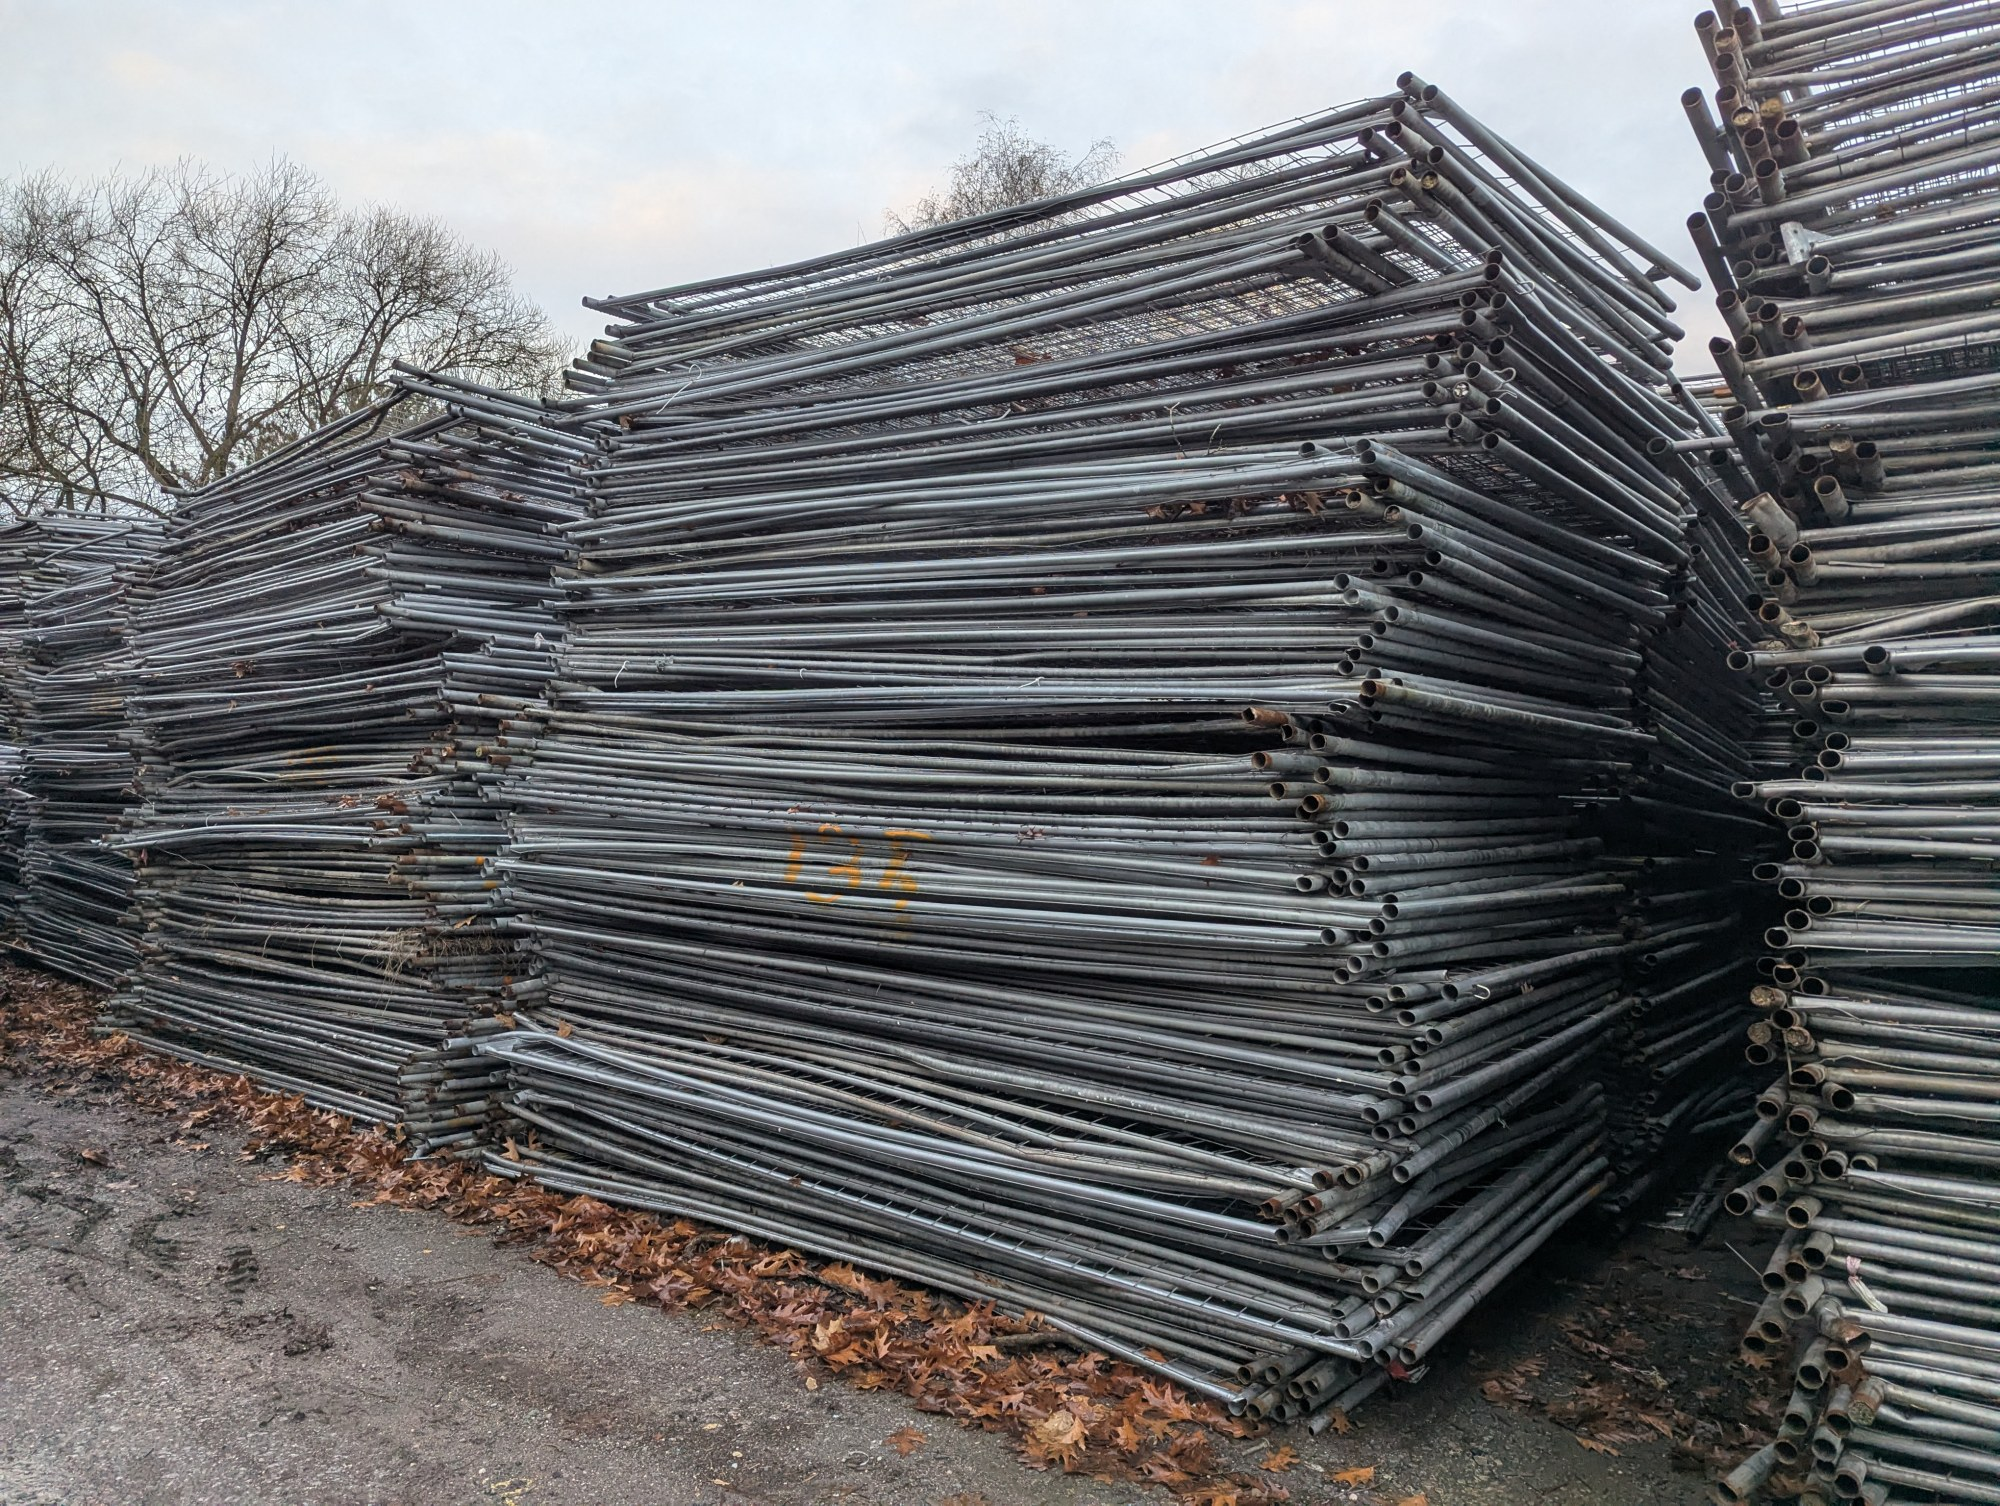
\includegraphics[width=0.92\textwidth]{abbildungen/real_stapel.jpg}
  \caption[Reale Stapelaufnahme]{Reale Aufnahme eines Stapels mobiler
  Bauzaunfelder. Zu detektieren ist die Stirnfläche der Rahmenrohre: heller
  verzinkter Kranz, dunkle Bohrung. Deutlich erkennbar sind die drei zentralen
  Schwierigkeiten -- geringe Objektgröße, hohe Objektdichte und wechselseitige
  Verdeckung durch quer liegende Rohrschäfte.}
  \label{abb:realstapel}
\end{figure}

Aus Sicht der Bildverarbeitung ist das ein unangenehmer Spezialfall: Die Objekte
sind klein (gemessen 12--36\px{} Durchmesser in den Originalaufnahmen), dicht
gepackt (im Median rund einen Objektdurchmesser Abstand zum nächsten Nachbarn),
untereinander nahezu identisch und wechselseitig verdeckt. Erschwerend kommt
hinzu, dass eine Zählaufgabe jeden einzelnen Detektionsfehler unmittelbar in das
Endergebnis überträgt: Für eine exakte Zählung von 200 Objekten wäre eine
Trefferquote von über 99,5\,\% erforderlich -- eine deutlich härtere Anforderung
als in typischen Detektionsanwendungen, in denen einzelne Fehldetektionen
tolerierbar sind.

Der eigentliche Engpass ist jedoch die Datenlage. COCO-vortrainierte Gewichte
enthalten keine Klasse \enquote{Bauzaunprofil}; das Modell muss auf einem eigens
annotierten Datensatz feinabgestimmt werden. Die Handannotation von 50--100
kleinen Boxen pro Bild über hunderte Bilder ist bei einer Abschlussarbeit nicht
leistbar. Zur Verfügung stehen lediglich neun aus Realbildern ausgeschnittene
Rohrprofile, sieben Hintergrundaufnahmen und zwei vollständig annotierte
Realbilder.

\section{Zielsetzung und Beitrag}

Der hier verfolgte Ansatz macht aus dieser Not das methodische Zentrum der
Arbeit: Trainiert wird \emph{ausschließlich} auf synthetischen Bildern, die aus
den neun Objektausschnitten und den sieben Hintergründen erzeugt werden.
Validierung und Test erfolgen auf den echten Aufnahmen. Damit ist die
Augmentierungs\-pipeline nicht mehr eine Menge von Zusatztransformationen auf einem
vorhandenen Datensatz, sondern sie \emph{ist} der Datensatz: Sie definiert die
gesamte Trainingsverteilung, und jede ihrer Entscheidungen wirkt direkt auf das
Ergebnis.

Die Arbeit verfolgt daher drei Ziele:

\begin{enumerate}
  \item \textbf{Theoretische Einordnung der Datenaugmentierung.} Was leistet
  Augmentierung formal, welche Verfahrensklassen gibt es, welche
  Besonderheiten gelten bei der Objektdetektion, und wo liegen die Grenzen?
  Kapitel~\ref{kap:augtheorie} behandelt dies unabhängig vom konkreten
  Anwendungsfall.
  \item \textbf{Vollständige Dokumentation und Begründung der konkreten
  Pipeline.} Für jede der 25 Transformationen werden Parameterbereich,
  gemessener Ist-Anteil im erzeugten Datensatz und Begründung angegeben
  (Kapitel~\ref{kap:pipeline} und \ref{kap:trainingszeit}). Die Begründung
  stützt sich dabei auf genau drei zulässige Quellen: eine Messung an den
  Realdaten, eine physikalische Randbedingung des Aufnahmegegenstands oder ein
  in der Literatur belegtes Argument. Wo keine dieser Quellen vorliegt, wird
  der Wert ausdrücklich als Annahme gekennzeichnet.
  \item \textbf{Experimentelle Bewertung.} Kapitel~\ref{kap:auswertung} misst,
  was die Pipeline auf echten Daten leistet, quantifiziert den
  Sim-to-Real-Abstand und prüft in einer kontrollierten Ablation, ob die
  aufwendigste Einzelentscheidung -- die Erzeugung physikalisch plausibler
  Verdeckung -- ihren Aufwand rechtfertigt.
\end{enumerate}

Der inhaltliche Beitrag liegt weniger in einer neuen Methode als in der
Konsequenz, mit der die Begründungspflicht durchgehalten wird. Copy-Paste-Synthese
ist ein etabliertes Verfahren \parencite{dwibedi2017,dvornik2018,ghiasi2021}; die
Frage, welche ihrer Bestandteile in einem konkreten industriellen Anwendungsfall
tragen und welche nicht, wird in der Literatur dagegen selten so kleinteilig
beantwortet, wie es hier versucht wird.

\section{Aufbau der Arbeit}

Kapitel~\ref{kap:theorie} stellt die theoretischen Grundlagen von Convolutional
Neural Networks und der YOLO26-Architektur bereit und leitet daraus die
Eignung des Verfahrens für die vorliegende Aufgabe ab.
Kapitel~\ref{kap:augtheorie} behandelt die Datenaugmentierung allgemein.
Kapitel~\ref{kap:daten} sichtet und vermisst das verfügbare Quellmaterial --
diese Messungen sind die Belegbasis für alle folgenden Parameterentscheidungen.
Kapitel~\ref{kap:pipeline} beschreibt die Synthese-Pipeline,
Kapitel~\ref{kap:trainingszeit} die davon abgegrenzte Augmentierung zur
Trainingszeit. Kapitel~\ref{kap:auswertung} wertet die Ergebnisse aus,
Kapitel~\ref{kap:diskussion} diskutiert Tragfähigkeit und Grenzen.

\begin{table}[htbp]
\centering
\caption[Verarbeitungskette]{Die Verarbeitungskette der Arbeit. Die Stufen 1--3
erzeugen die Trainingsdaten und sind Gegenstand von
Kapitel~\ref{kap:pipeline}.}
\label{tab:kette}
\small
\begin{tabularx}{\textwidth}{@{}llX@{}}
\toprule
\textbf{Stufe} & \textbf{Skript} & \textbf{Aufgabe} \\
\midrule
0 & \code{analyze\_data.py} & Sichtung und Vermessung des Quellmaterials; erzeugt
alle Messwerte, auf die sich die Parameterbegründungen berufen \\
1 & \code{matting.py} & Freistellen der neun Objektausschnitte, weiche Alphamasken \\
2 & \code{occluders.py} & Extraktion echter Rohrschäfte als Okkluder-Bibliothek \\
3 & \code{generate.py} & Bildsynthese mit exakter Sichtbarkeitsrechnung \\
4 & \code{train.py} & Training, Parametertabelle mit Begründungen \\
5 & \code{evaluate.py} & eigenständiges Bewertungsframework (COCO-Metriken, Zählfehler) \\
6 & \code{experiment.py} & Inferenzparameter-Sweeps, Okklusionsablation, Modellvergleich \\
7 & \code{report.py} & Diagramme und Ergebnistabellen \\
\bottomrule
\end{tabularx}
\end{table}

\chapter{Theoretische Grundlagen}
\label{kap:theorie}

\section{Convolutional Neural Networks}
\label{sec:cnn}

\subsection{Grundprinzipien}
\label{sec:prinzipien}

Convolutional Neural Networks beruhen auf drei Prinzipien: \emph{lokale
rezeptive Felder}, \emph{geteilte Gewichte} und \emph{räumliche
Unterabtastung}. Sie sind keine Implementierungsdetails, sondern kodieren
strukturelles Vorwissen über Bilddaten in die Netzarchitektur -- Lokalität,
Stationarität und Toleranz gegenüber kleinen Verschiebungen
\parencite{lecun1998,goodfellow2016}.

\absatz{Lokale rezeptive Felder und geteilte Gewichte.} Statt jedes
Ausgabeneuron mit allen $H \cdot W$ Eingangspixeln zu verbinden, beschränkt eine
Faltungsschicht die Summation auf eine $k \times k$-Nachbarschaft und verwendet
denselben Kernel an allen Positionen. Die Parameterzahl einer Schicht wird
dadurch unabhängig von der Bildgröße, und dasselbe Muster wird überall erkannt,
auch wenn es in den Trainingsdaten nur an wenigen Positionen vorkommt. Der
belastbare Vorteil liegt in dieser \emph{Stichprobeneffizienz}, nicht in der
Kapazitätsbeschränkung: \textcite{zhang2017rethinking} zeigen, dass gängige
Faltungsnetze zufällige Beschriftungen vollständig memorieren können und dennoch
generalisieren. Die Operation ist \emph{translationsäquivariant} -- eine
verschobene Eingabe erzeugt eine identisch verschobene Ausgabe --, was durch die
näherungsweise Stationarität natürlicher Bildstatistik gerechtfertigt ist. Die Faltung
 ist dabei translationsäquivariant, während nachfolgendes Downsampling die räumliche
 Präzision reduziert und dadurch eine gewisse Robustheit gegenüber kleinen Verschiebungen 
 erzeugen kann

\absatz{Räumliches Subsampling -- die für diese Arbeit entscheidende Stufe.} Für
die Objekterkennung ist Invarianz gegenüber kleinen Verschiebungen erwünscht.
Sie entsteht durch stufenweise Reduktion der räumlichen Auflösung -- klassisch
durch Max-Pooling, in modernen Architekturen wie YOLO26 überwiegend durch
Faltungen mit Schrittweite $s = 2$. Erhalten bleibt dabei nur, \emph{ob} ein
Merkmal im Fenster auftrat, nicht seine exakte Position. Nach $L$ solchen Stufen
beträgt die \textbf{Gesamtschrittweite} $S = \prod_\ell s_\ell = 2^L$.

Der Preis ist ein Verlust an Ortsinformation, und der wird bei kleinen Objekten
kritisch. Eine Zelle der Merkmalsebene mit Gesamtschrittweite $S$ entspricht
einem Bildbereich von $S \times S$ Pixeln; ein Objekt mit Durchmesser $d$ belegt
dort nur $d/S$ Zellen. Für \(d<S\) erstreckt sich das Objekt im Mittel über weniger
 als eine Gitterzelle und ist damit nur durch sehr wenige räumliche Positionen repräsentiert.
  Eine zuverlässige Lokalisierung wird dadurch zunehmend erschwert. Für die feinste
Standard-Detektionsebene P3 in YOLO26 gilt $S = 8$ -- das kleinste Rohrprofil in
\code{test} misst 6,4 Pixel und unterschreitet diese Grenze. „Das Verhältnis \(d/S\) 
dient in dieser Arbeit als zentrale geometrische Kenngröße für die räumliche Repräsentierbarkeit
 kleiner Objekte es begründet
die Multi-Skalen-Fusion moderner Detektoren (Abschnitt~\ref{sec:neck}) und die
drei möglichen Gegenmaßnahmen, die alle dasselbe Verhältnis vergrößern: Eine
höhere Eingabeauflösung und Kachelung erhöhen $d$, ein zusätzlicher
Detektionskopf senkt $S$ (Abschnitt~\ref{sec:p2kopf}).

\subsection{Merkmalshierarchie und Objektdetektion}
\label{sec:hierarchie}

Auf jede Faltung folgt eine nichtlineare Aktivierung -- heute überwiegend die
Rectified Linear Unit $f(x) = \max(0,x)$ oder Varianten wie SiLU
\parencite{krizhevsky2012} --, ohne die das Netz nur lineare Abbildungen lernen
könnte. Aus der Stapelung entsteht ein hierarchischer Aufbau der
Repräsentationen: Frühe Schichten reagieren auf Kanten und Farbverläufe, mittlere
auf Texturen und Teilstrukturen, tiefe auf semantische Objektbestandteile
\parencite{zeiler2014}. Diese datengetriebene Merkmalsextraktion tritt an die
Stelle des manuell entworfenen Feature Engineering und gilt als wesentlicher
Grund für die Leistungssprünge tiefer Netze \parencite{lecun2015}. Am Ende
klassischer Architekturen fassen vollvernetzte Schichten die Merkmale zusammen;
in modernen Detektoren sind sie vollständig durch Faltungen ersetzt
(Abschnitt~\ref{sec:neck}). Residualverbindungen \parencite{he2016} ermöglichen
das stabile Training sehr tiefer Netze und sind Standardbaustein nahezu aller
CNN-Backbones.

Für diese Arbeit ist nicht die Klassifikation relevant, sondern die
\textbf{Objektdetektion}: das gleichzeitige Lokalisieren und Klassifizieren
mehrerer Objekte. Zweistufige Detektoren erzeugen zunächst Regionsvorschläge und
klassifizieren diese anschließend \parencite{ren2015}; einstufige Detektoren
formulieren die Detektion als einmaliges Regressionsproblem und sagen in einem
Durchlauf direkt Boxen und Klassenwahrscheinlichkeiten vorher
\parencite{redmon2016,liu2016ssd}, was Echtzeitfähigkeit bei geringen
Genauigkeitseinbußen ermöglicht. Klassisch nachgeschaltet ist die
Non-Maximum Suppression (NMS), die redundante überlappende Detektionen anhand
ihrer Intersection over Union unterdrückt -- bei dicht gepackten gleichartigen
Objekten eine potenzielle Fehlerquelle.

\section{YOLO26}
\label{sec:yolo26}

\subsection{Einordnung}

\enquote{You Only Look Once} wurde 2016 als erster echtzeitfähiger einstufiger
Detektor vorgestellt \parencite{redmon2016}; ab YOLOv8 übernahm Ultralytics die
Weiterentwicklung und etablierte ankerfreie, entkoppelte Detektionsköpfe
\parencite{sapkota2025}. YOLO26 wurde im September 2025 vorgestellt und
unterscheidet sich von YOLO11 durch vier koordinierte Änderungen: ein
Dual-Head-Design für NMS-freie Inferenz, den Wegfall der Distribution Focal Loss,
ProgLoss zusammen mit STAL sowie den MuSGD-Optimierer
\parencite{jocher2026yolo26,sapkota2025}.

Für diese Arbeit ist davon eine Änderung einschlägig: Die
\emph{Small-Target-Aware Label Assignment} garantiert positive Labelzuweisungen
auch für sehr kleine Objekte -- genau das Problem klassischer
Zuweisungsstrategien, das Abschnitt~\ref{sec:ioukleinobjekt} quantifiziert.

\subsection{Backbone, Neck, Head und die Merkmalspyramide}
\label{sec:neck}

YOLO26 folgt der Dreiteilung \textbf{Backbone $\to$ Neck $\to$ Head}. Das
Backbone reduziert die räumliche Auflösung stufenweise per Stride-2-Faltungen
($1024 \to 512 \to 256 \to 128 \to 64 \to 32$ bei $1024$\px{} Eingabe), während
die Kanalzahl wächst -- räumliche Präzision wird gegen semantische Tiefe
getauscht.

\absatz{Neck.} Das Neck verbindet die Auflösungsstufen in beide Richtungen
(FPN/PAN-Prinzip, \cite{lin2017fpn}): Tiefe, semantisch reiche Merkmalskarten
werden hochskaliert und mit den feinen, ortsgenauen Karten früherer Stufen
zusammengeführt, und umgekehrt. Der Head erhält dadurch mehrere Ausgabeebenen,
die nach Objektgröße zuständig sind. Die Standardkonfiguration liefert drei
Ebenen P3/P4/P5 mit den Gesamtschrittweiten 8/16/32; zusätzlich existiert eine
Konfiguration mit einer vierten, feineren Ebene \textbf{P2 mit Schrittweite~4}
(Abbildung~\ref{abb:pyramide}). Diese Variante wird hier durchgängig verwendet;
Abschnitt~\ref{sec:p2kopf} begründet, warum.

\begin{figure}[htbp]
\centering
\begin{tikzpicture}[x=1cm,y=1cm]
  % ---- Merkmalsebenen als Quadrate, Seitenlaenge proportional zur Gittergroesse
  \draw[fill=red!8,dashed,thick,red!60!black] (0,0) rectangle (4,4);
  \draw[step=0.5,gray!35,very thin] (0,0) grid (4,4);
  \draw[fill=blue!8] (4.7,0) rectangle (6.7,2);
  \draw[step=0.5,gray!35,very thin] (4.7,0) grid (6.7,2);
  \draw[fill=blue!8] (7.4,0) rectangle (8.4,1);
  \draw[step=0.5,gray!35,very thin] (7.4,0) grid (8.4,1);
  \draw[fill=blue!8] (9.1,0) rectangle (9.6,0.5);

  \node[below,align=center,font=\scriptsize] at (2,-0.2)
       {\textbf{P2} $\;$ Stride 4\\$256\times256$\\65\,536 Positionen};
  \node[below,align=center,font=\scriptsize] at (5.7,-0.2)
       {\textbf{P3} $\;$ Stride 8\\$128\times128$\\16\,384};
  \node[below,align=center,font=\scriptsize] at (7.9,-0.2)
       {\textbf{P4} $\;$ 16\\$64^2$\\4\,096};
  \node[below,align=center,font=\scriptsize] at (9.35,-0.2)
       {\textbf{P5} $\;$ 32\\$32^2$\\1\,024};

  \node[above,font=\scriptsize,red!60!black,align=center] at (2,4.15)
       {\emph{zusätzlich in} \code{-p2}, \emph{hier verwendet}};
  \node[above,font=\scriptsize,align=center] at (7.0,4.15)
       {Standardkonfiguration P3--P5};
  \draw[decorate,decoration={brace,amplitude=4pt},gray!60!black]
       (4.7,4.05) -- (9.6,4.05);
  \node[font=\scriptsize,align=left,anchor=west] at (10.1,2.6)
       {kleine\\Objekte};
  \node[font=\scriptsize,align=left,anchor=west] at (10.1,1.2)
       {große\\Objekte};
  \draw[-{Latex[length=1.6mm]},gray!60!black] (10.35,2.3) -- (10.35,1.6);
\end{tikzpicture}
\caption[Merkmalsebenen des Detektionskopfes]{Merkmalsebenen des
Detektionskopfes bei einer Eingabe von $1024\times1024$ Pixeln. Die
Seitenlänge der Quadrate ist proportional zur Gittergröße. Jede Zelle einer
Ebene mit Schrittweite $S$ entspricht einem Bildbereich von $S \times S$ Pixeln
und sagt Boxkoordinaten sowie Klassen-Scores vorher. Die Standardkonfiguration
nutzt \textbf{P3--P5}; die hier trainierten Modelle verwenden zusätzlich die
links rot gestrichelt eingezeichnete Ebene \textbf{P2} mit Schrittweite~4. Die
Abbildung zeigt zugleich, warum diese eine Ebene so viel ausmacht: P2 allein
enthält mehr Prädiktionspositionen als P3, P4 und P5 zusammen. Genau diese
Abhängigkeit von der Schrittweite macht Abschnitt~\ref{sec:ioukleinobjekt} zum
Kern des Auflösungsproblems.}
\label{abb:pyramide}
\end{figure}

\absatz{Head.} Der Kopf ist vollständig faltungsbasiert: kleine
Faltungsstapel, die in $1\times1$-Faltungen münden. Eine $1\times1$-Faltung ist
äquivalent zu einer vollvernetzten Schicht über die Kanaldimension, wird aber
\textbf{positionsgeteilt} angewendet -- dieselbe Operation verarbeitet die Kanäle
jeder Gitterzelle separat. Das erhält die Translationsäquivarianz bis in die
Ausgabeschicht und macht das Netz unabhängig von einer festen Eingabegröße. Der
Kopf ist zusätzlich
\emph{entkoppelt} (getrennte Zweige für Klassifikation und Boxregression) und
\emph{ankerfrei}: Jede Gitterzelle regressiert direkt die Abstände zu den vier
Boxrändern. Damit ist die Zahl der Gitterzellen -- und nicht die Zahl der
Ankerboxen -- die Größe, die bestimmt, wie fein Objekte überhaupt aufgelöst
werden können.

\subsection{Der P2-Detektionskopf}
\label{sec:p2kopf}

Alle in dieser Arbeit trainierten Modelle sind \code{yolo26s-p2}. Diese Wahl ist
kein Gegenstand der Experimente, sondern deren Konstante; sie ist an dieser
Stelle zu begründen, weil sie unmittelbar an der Auflösungsgrenze hängt, die
Abschnitt~\ref{sec:ioukleinobjekt} herleitet.

\absatz{} Der Unterschied liegt allein im Neck und im Kopf. Die
Standardkonfiguration führt den Aufwärtspfad des Feature-Pyramid-Netzwerks
\parencite{lin2017fpn} bis P3 und schickt von dort einen Abwärtspfad über P4 zu
P5; die \code{-p2}-Variante setzt den Aufwärtspfad um eine Stufe fort, verknüpft
ihn mit der P2-Karte des Backbones und startet den Abwärtspfad eine Ebene tiefer.
Der Detektionskopf erhält vier statt drei Eingänge. Weil die Eingangsbreite des
Kopfes seine internen Kanalzahlen bestimmt und der neue, feinste Eingang schmaler
ist als der bisherige, hat die Variante sogar \emph{weniger} Parameter als das
Basismodell: 9\,663\,464 gegen 9\,948\,638, also $-2{,}9\,\%$. Alle Kennzahlen
dieses Absatzes stammen aus der Modellzusammenfassung, die die Werkzeugkette beim
Aufbau der beiden Netze ausgibt; Speicher und Laufzeit sind an den eigenen
Trainingsläufen gemessen. Sie ist kein
größeres, sondern ein \emph{feiner aufgelöstes} Netz.

\absatz{}Die Prädiktionspositionen sind die Summe der
Gitterzellen aller Detektionsebenen und damit aus der Eingabegröße abzählbar: Bei
$1024\times1024$ vervierfachen sie sich von $128^2+64^2+32^2 = 21\,504$ auf
$256^2 + 21\,504 = 87\,040$. Der Rechenaufwand steigt dagegen nur um 17\,\%
(22,7 auf 26,6 GFLOPs bei $640^2$, laut Modellzusammenfassung), weil die zusätzlichen Blöcke
auf der feinsten Ebene schmal sind. Teuer ist der \emph{Speicher}: Er wird von
den Aktivierungen dominiert, und eine Merkmalskarte auf P2 hat viermal so viele
Positionen wie eine auf P3. Gemessen belegt das Training bei \code{imgsz}=1024
mit Batch~8 rund 12\,GB statt etwa 6\,GB. Das ist der eigentliche Preis der
Variante und der Grund, warum sie nicht der Standard ist.

\absatz{Nutzen} Der Nutzen lässt sich vor jedem Training abschätzen.
Nach Gleichung~\eqref{eq:zellen} beträgt die erwartete Zahl der Gitterzellen,
deren Zentrum in ein kreisförmiges Objekt vom Durchmesser $d$ fällt und die damit
überhaupt als positive Zuweisung in Frage kommen, $\mathbb{E}[N] = \pi d^2/(4S^2)$;
der Übergang von $S = 8$ auf $S = 4$ vervierfacht diesen Wert.
Tabelle~\ref{tab:p2zellen} setzt ihn für die tatsächlich auftretenden
Objektgrößen ein. Entscheidend ist nicht der Mittelwert, sondern die Spalte
\enquote{min}: Bei $S = 8$ hat das kleinste Objekt in \code{test} im
ungünstigsten Fall \emph{genau eine} Kandidatenzelle -- eine einzige Position,
die es finden kann --, bei $S = 4$ sind es vier. Die Zuweisungsgrenze
$d < S\sqrt{2}$ sinkt von 11,3\px{} auf 5,7\px{} und liegt damit vollständig
unterhalb der hier auftretenden Objektgrößen.

\begin{table}[htbp]
\centering
\caption[Kandidatenzellen je Objekt]{Erwartete Zahl der Gitterzellen, deren
Zentrum in das Objekt fällt, nach Gleichung~\eqref{eq:zellen}, bei nativem
Maßstab. Die Spalte \enquote{min} nennt den ungünstigsten Fall über alle Lagen
des Objektzentrums im Gitter; sie hat keine geschlossene Form und ist durch
Absuchen der Lagen auf einem feinen Raster bestimmt.}
\label{tab:p2zellen}
\footnotesize
\begin{tabular}{@{}rlrrrr@{}}
\toprule
$d$ (px) & Bedeutung & \multicolumn{2}{c}{P3 ($S=8$)} &
\multicolumn{2}{c}{P2 ($S=4$)} \\
 & & Mittel & min & Mittel & min \\
\midrule
11,6 & p05 des synthetischen Datensatzes & 1,7 & 1 & 6,6 & 4 \\
12,2 & kleinstes Objekt in \code{test}   & 1,8 & 1 & 7,3 & 4 \\
19,6 & Median \code{test}                & 4,7 & 4 & 18,9 & 16 \\
22,5 & Median des synthetischen Datensatzes & 6,2 & 4 & 24,9 & 21 \\
27,4 & Median \code{val}                 & 9,2 & 8 & 36,9 & 32 \\
\bottomrule
\end{tabular}
\end{table}

\absatz{} Ein Detektor, dem die
Auflösung fehlt, übersieht kleine Objekte unabhängig davon, wie gut seine
Trainingsdaten sind. Jede Verbesserung der Datenerzeugung würde dann teilweise
nur eine Architekturschwäche kompensieren, und der gemessene Effekt wäre nicht
der Effekt der Daten. Die Ablationen der Kapitel~\ref{kap:auswertung} laufen
deshalb auf der feiner aufgelösten Variante -- nicht, weil sie besser
\emph{aussieht}, sondern weil sie die Störgröße entfernt, die den Datengewinn
sonst überlagert.

\section{Anwendung auf gestapelte Bauzaunprofile}
\label{sec:anwendung}

Ein YOLO-Modell wird per Transfer Learning von COCO-vortrainierten Gewichten
\parencite{yosinski2014} auf eine einzige Objektklasse feinabgestimmt. Zwei
Eigenschaften von YOLO26 passen dabei unmittelbar zum Problem: STAL und ProgLoss
verbessern die Erkennung kleiner Objekte, und die NMS-freie Inferenz eliminiert
einen bei dicht gepackten gleichartigen Objekten systematisch fehleranfälligen
Hyperparameter -- ein zu niedriger IoU-Schwellwert unterdrückt korrekte
Detektionen benachbarter Rohre, ein zu hoher lässt Duplikate zu.

Drei Grenzen bleiben und strukturieren den Praxisteil. Die \textbf{Auflösung}
(Abschnitt~\ref{sec:prinzipien}) wird über den P2-Kopf und die Inferenzauflösung
adressiert (Abschnitte~\ref{sec:p2kopf} und~\ref{sec:imgsz}); die
\textbf{Verdeckung} -- verkippte Zäune verdecken benachbarte Profile, und
Gitterknoten, Löcher im Maschendraht und Schattenspalten drohen als
Falschpositive -- ist Gegenstand der Ablation in Abschnitt~\ref{sec:ablationB};
und der \textbf{Datenbedarf} wird nicht durch Handannotation gedeckt, sondern
durch eine Synthese-Pipeline, deren Entwurf die Kapitel~\ref{kap:augtheorie}
bis~\ref{kap:trainingszeit} füllt.

\chapter{Datenaugmentierung -- theoretische Grundlagen}
\label{kap:augtheorie}

Der Praxisteil dieser Arbeit steht und fällt mit der Augmentierung. Dieses
Kapitel entwickelt daher zunächst unabhängig vom konkreten Anwendungsfall, was
Augmentierung formal leistet (Abschnitt~\ref{sec:augformal}), über welche
Mechanismen sie wirkt (Abschnitt~\ref{sec:augmechanismen}), welche
Verfahrensklassen sich etabliert haben (Abschnitt~\ref{sec:augtaxonomie}), welche
Besonderheiten bei der Objektdetektion gelten
(Abschnitt~\ref{sec:augdetektion}) und wo die Grenzen des Verfahrens liegen
(Abschnitt~\ref{sec:auggrenzen}). Abschnitt~\ref{sec:augsynthese} behandelt den
Grenzfall, um den es hier geht: Augmentierung, die die Trainingsverteilung nicht
erweitert, sondern vollständig erzeugt. Aus diesem Kapitel werden am Ende sechs
Anforderungen abgeleitet, an denen sich die konkrete Pipeline in
Kapitel~\ref{kap:pipeline} messen lässt.

\section{Begriff und formale Einordnung}
\label{sec:augformal}

\absatz{Definition.} Datenaugmentierung bezeichnet die künstliche Vergrößerung
eines Trainingsdatensatzes durch Transformationen, die den semantischen Gehalt
der Beispiele -- und damit ihre Beschriftung -- erhalten
\parencite{shorten2019}. Formal sei
$D = \{(x_i, y_i)\}_{i=1}^{n}$ der Trainingsdatensatz, $\mathcal{T}$ eine Familie
von Transformationen mit einer Verteilung $p(t)$ über $\mathcal{T}$, und
$\tau_t$ die zu $t$ gehörende \emph{Labeltransformation}. Anstelle des
empirischen Risikos
\begin{equation}
\hat{R}(f) \;=\; \frac{1}{n}\sum_{i=1}^{n} L\big(f(x_i),\, y_i\big)
\label{eq:erm}
\end{equation}
minimiert das Training dann das \emph{augmentierte} Risiko
\begin{equation}
\hat{R}_{\text{aug}}(f) \;=\; \frac{1}{n}\sum_{i=1}^{n}
\mathbb{E}_{t \sim p(t)}\Big[ L\big(f(t(x_i)),\, \tau_t(y_i)\big) \Big].
\label{eq:erm-aug}
\end{equation}

Zwei Punkte an Gleichung~\eqref{eq:erm-aug} sind für das Weitere zentral. Erstens
tritt neben $t$ stets die Labeltransformation $\tau_t$ auf. Bei der
Bildklassifikation ist $\tau_t = \mathrm{id}$ -- eine gespiegelte Katze bleibt
eine Katze --, weshalb Augmentierung dort begrifflich mit
\enquote{label-erhaltend} gleichgesetzt wird. Bei der Objektdetektion ist
$\tau_t \neq \mathrm{id}$: Boxkoordinaten müssen mittransformiert werden, und
genau dabei entstehen die in Abschnitt~\ref{sec:augdetektion} behandelten Fehler.
Zweitens ist $p(t)$ ein Modellierungsgegenstand und keine Nebensache: Sie legt
fest, \emph{wie häufig} und \emph{wie stark} eine Transformation auftritt. Die
vollständige Dokumentation von $p(t)$ ist damit die Mindestanforderung an eine
reproduzierbare Augmentierung -- und der Grund, warum in
Kapitel~\ref{kap:pipeline} für jede Transformation nicht nur der
Parameterbereich, sondern auch der gemessene Ist-Anteil angegeben wird.

\absatz{Verhältnis zur Vicinal Risk Minimization.} Gleichung~\eqref{eq:erm-aug}
lässt sich auch so lesen, dass jeder Datenpunkt durch eine \emph{Umgebung}
(\enquote{vicinity}) ersetzt wird, über die das Risiko gemittelt wird.
\textcite{chapelle2001} formalisieren dies als Vicinal Risk Minimization: Statt
der empirischen Verteilung $\hat{P}(x,y) = \frac{1}{n}\sum_i
\delta(x-x_i)\delta(y-y_i)$ wird eine geglättete Verteilung
$\hat{P}_{\text{vic}}$ verwendet, deren Träger über die Datenpunkte hinausreicht.
Augmentierung ist damit die anwendungsspezifische Wahl dieser Umgebung: Sie
kodiert, welche Nachbarschaft eines Beispiels als \enquote{dasselbe Objekt} gilt.
Verfahren wie \emph{mixup} \parencite{zhang2018mixup} berufen sich explizit auf
diesen Rahmen.

\absatz{Verhältnis zum induktiven Bias der Architektur.}
Abschnitt~\ref{sec:prinzipien} hat gezeigt, dass die Faltungsarchitektur
Translationsäquivarianz \emph{strukturell} garantiert
(Gleichung~\eqref{eq:aequivarianz}). Für alle anderen erwünschten Invarianzen --
Rotation, Skalierung, Beleuchtung, Farbstich, Teilverdeckung -- gibt es in einem
gewöhnlichen CNN keine solche Garantie; sie müssen aus Daten gelernt werden.
Augmentierung ist genau das Werkzeug, mit dem diese Invarianzen auf der
\emph{Datenseite} statt auf der Architekturseite eingebracht werden. Die
Arbeitsteilung lässt sich damit so zusammenfassen:

\begin{itemize}
  \item \textbf{Architektur:} Lokalität, Stationarität, Translationsäquivarianz
  (Faltung), begrenzte Translationsinvarianz (Subsampling).
  \item \textbf{Augmentierung:} alle übrigen Invarianzen der konkreten Domäne --
  und nur diese; jede Invarianz, die in der Domäne \emph{nicht} gilt, darf nicht
  antrainiert werden.
\end{itemize}

Der zweite Halbsatz ist der wesentliche Entwurfsgrundsatz. Eine
Augmentierung, die eine in der Realität nicht vorhandene Invarianz erzwingt,
verschlechtert das Modell, weil sie diskriminative Information entfernt. Ein
Beispiel aus dem vorliegenden Fall: Volle Rotationsinvarianz ist bei einem
Rohrende korrekt, weil Kamerarollwinkel und Stapelausrichtung beliebig sind. Bei
einem Verkehrszeichen wäre sie falsch.

\section{Wirkmechanismen}
\label{sec:augmechanismen}

Die Literatur nennt drei voneinander unterscheidbare Mechanismen, über die
Augmentierung die Generalisierung verbessert. Sie treten in der Praxis
gemeinsam auf, haben aber unterschiedliche Voraussetzungen.

\absatz{(1) Kodierung von Invarianzen und Varianzreduktion.} Bildet
$\mathcal{T}$ eine Gruppe $G$, unter deren Wirkung die Beschriftung invariant
ist, so entspricht die Mittelung in Gleichung~\eqref{eq:erm-aug} einer Projektion
des Schätzers auf den Raum der $G$-invarianten Funktionen.
\textcite{chen2020group} zeigen, dass diese Orbit-Mittelung die Varianz des
Schätzers nachweisbar reduziert, ohne den Bias zu erhöhen -- Augmentierung ist in
diesem Rahmen also strikt vorteilhaft, sofern die angenommene Invarianz
tatsächlich gilt. \textcite{dao2019} kommen über eine Kernel-Approximation zu
einer verwandten Zerlegung: Augmentierung wirkt zum Teil als Mittelung über die
Gruppenbahn (Invarianzterm), zum Teil als datenabhängige Regularisierung
(Varianzterm).

\absatz{(2) Regularisierung durch Rauschen.} Nicht jede Augmentierung ist eine
Gruppenoperation. Photometrische Störungen, Rauschen und Unschärfe sind
Perturbationen ohne Gruppenstruktur. Für den Grenzfall kleiner additiver
Störungen zeigt \textcite{bishop1995}, dass Training mit Rauschen äquivalent zu
einer Tikhonov-Regularisierung ist: Der Erwartungswert des gestörten
Fehlerfunktionals enthält in zweiter Ordnung einen Strafterm auf den Ableitungen
der Netzfunktion. Augmentierung dieser Art glättet die gelernte Funktion also
messbar, statt lediglich \enquote{mehr Daten} zu erzeugen.

\absatz{(3) Erweiterung des Trägers der Trainingsverteilung.} Der praktisch
wichtigste, theoretisch am schwächsten fassbare Mechanismus: Augmentierung
erzeugt Konfigurationen, die im Originaldatensatz überhaupt nicht vorkommen --
Objekte in Größen, Orientierungen, Beleuchtungen und Verdeckungsgraden, die die
Aufnahmesituation nicht geliefert hat. Bei einem Datensatz mit sehr wenigen
Quellobjekten -- neun im vorliegenden Fall -- ist dies der dominierende Effekt:
Ohne diesen Mechanismus wäre der Datensatz auf neun Erscheinungsbilder
beschränkt. Die Grenze des Mechanismus ist gleichzeitig offensichtlich:
Augmentierung erzeugt keine neue \emph{Information} über die Objektklasse,
sondern verteilt die vorhandene Information über einen größeren Bereich des
Eingaberaums \parencite{shorten2019}.

\section{Taxonomie der Verfahren}
\label{sec:augtaxonomie}

Tabelle~\ref{tab:taxonomie} ordnet die etablierten Verfahren nach dem
Mechanismus, über den sie wirken. Die Einteilung ist nicht disjunkt -- Mosaic
etwa wirkt gleichzeitig über Skalenvariation und über Kontextvermischung --,
strukturiert aber die Entwurfsentscheidungen der folgenden Kapitel.

\begin{table}[htbp]
\centering
\caption[Taxonomie der Augmentierungsverfahren]{Verfahrensklassen der
Bildaugmentierung. Die letzte Spalte gibt an, ob und wie das Verfahren im
vorliegenden Anwendungsfall eingesetzt wird; die Begründungen folgen in den
Kapiteln~\ref{kap:pipeline} und \ref{kap:trainingszeit}.}
\label{tab:taxonomie}
\scriptsize
\begin{tabularx}{\textwidth}{@{}L{0.20\textwidth}L{0.30\textwidth}L{0.20\textwidth}X@{}}
\toprule
\textbf{Klasse} & \textbf{Verfahren (Auswahl)} & \textbf{Quelle} &
\textbf{Einsatz hier} \\
\midrule
Geometrisch, global &
Spiegelung, Rotation, Skalierung, Translation, Scherung, Perspektive,
elastische Verzerrung &
\cite{krizhevsky2012}; \cite{simard2003} &
Spiegelung, Skalierung, Translation: ja. Rotation/Scherung/Perspektive
\emph{global}: nein (Labelrauschen, Abschnitt~\ref{sec:augdetektion}) \\
\addlinespace
Geometrisch, pro Instanz &
Rotation, anisotrope Skalierung, Homographie einzelner Objekte &
\cite{dwibedi2017}; \cite{ghiasi2021} &
ja, im Generator mit exakter Neuberechnung der Box \\
\addlinespace
Photometrisch &
Helligkeit, Kontrast, Gamma, HSV-Verschiebung, Weißabgleich, PCA-Farbrauschen &
\cite{krizhevsky2012}; \cite{grossberg2003} &
ja, zweistufig (pro Instanz und global) \\
\addlinespace
Degradation &
Unschärfe, Bewegungsunschärfe, Sensorrauschen, JPEG-Requantisierung,
Vignettierung &
\cite{hendrycks2019} &
ja; hier zusätzlich als Mittel gegen Einfügeartefakte
(Abschnitt~\ref{sec:augsynthese}) \\
\addlinespace
Informationsentzug (Okklusion) &
Cutout, Random Erasing, Hide-and-Seek, GridMask &
\cite{devries2017cutout}; \cite{zhong2020erasing}; \cite{singh2017hideseek} &
nein in der generischen Form; ersetzt durch physikalisch motivierte Verdeckung
(Abschnitt~\ref{sec:okklusion}) \\
\addlinespace
Mehrbild-Mischung &
mixup, CutMix, Mosaic &
\cite{zhang2018mixup}; \cite{yun2019cutmix}; \cite{bochkovskiy2020} &
nur Mosaic; mixup/CutMix aus. Begründung in
Abschnitt~\ref{sec:trainparam} \\
\addlinespace
Gelernte Strategien &
AutoAugment, RandAugment, TrivialAugment, Detektions-Policies &
\cite{cubuk2019}; \cite{cubuk2020}; \cite{mueller2021}; \cite{zoph2020} &
nein -- setzt einen Suchsplit voraus, der hier nicht existiert
(Abschnitt~\ref{sec:autoaug}) \\
\addlinespace
Synthese (Copy-Paste) &
Einkopieren freigestellter Objekte in reale Hintergründe &
\cite{dwibedi2017}; \cite{dvornik2018}; \cite{ghiasi2021} &
ja -- Kern des Verfahrens \\
\addlinespace
Synthese (Rendering) &
Domain Randomization, strukturierte Domänenrandomisierung, physikbasiertes
Rendering &
\cite{tobin2017}; \cite{tremblay2018}; \cite{prakash2019} &
konzeptionell übernommen, technisch nicht (kein 3D-Modell verfügbar) \\
\addlinespace
Generative Modelle &
Diffusionsmodelle als Augmentierer &
\cite{trabucco2024} &
nein -- Boxtreue nicht garantiert, Rechenaufwand \\
\bottomrule
\end{tabularx}
\end{table}

\absatz{Zur Umsetzung.} Für die Klassen \enquote{geometrisch},
\enquote{photometrisch} und \enquote{Degradation} stehen fertige Bibliotheken
bereit; die verbreitetste ist Albumentations \parencite{buslaev2020}, die
Transformationen einschließlich der Boxtransformation kapselt. Für die
vorliegende Arbeit ist sie dennoch nicht verwendet worden, weil die zentrale
Anforderung -- eine exakte Sichtbarkeitsbuchhaltung über die Malreihenfolge
mehrerer eingefügter Objekte (Abschnitt~\ref{sec:sichtbarkeit}) -- außerhalb des
Funktionsumfangs solcher Bibliotheken liegt. Die bildweiten Transformationen
liefert die Trainingswerkzeugkette selbst (Kapitel~\ref{kap:trainingszeit}).

\absatz{Zur Rolle der Okklusionsverfahren.} Eine Untergruppe verdient besondere
Beachtung, weil sie im vorliegenden Fall eine eigene Pipelinestufe rechtfertigt.
Cutout \parencite{devries2017cutout}, Random Erasing
\parencite{zhong2020erasing} und Hide-and-Seek \parencite{singh2017hideseek}
löschen zufällige Bildbereiche. Die Begründung ist in allen drei Arbeiten
dieselbe: Ein Netz, das ein Objekt an einem einzigen besonders diskriminativen
Teilmerkmal erkennt, bricht ein, sobald dieses Merkmal verdeckt ist; wird im
Training regelmäßig Information entzogen, muss das Netz die Evidenz über das
gesamte Objekt verteilen. \textcite{wang2017afastrcnn} erzeugen zu diesem Zweck
Verdeckungen sogar adversarial, also gezielt an der für den aktuellen Detektor
schädlichsten Stelle; \textcite{kortylewski2020} zeigen komplementär, dass
Okklusionsrobustheit auch architektonisch erreichbar ist. Im vorliegenden
Anwendungsfall ist Verdeckung nicht bloß eine Regularisierungsidee, sondern der
Normalfall der Zieldomäne: In den Realbildern verdecken quer liegende Rohre und
benachbarte Profile einen erheblichen Teil der Stirnflächen. Die Pipeline erzeugt
Verdeckung daher nicht durch gelöschte Rechtecke, sondern durch physikalisch
plausible Okkluder -- mit dem entscheidenden Zusatznutzen, dass die Sichtbarkeit
dabei exakt berechnet und in die Labelentscheidung überführt werden kann
(Abschnitt~\ref{sec:sichtbarkeit}).

\section{Besonderheiten bei der Objektdetektion}
\label{sec:augdetektion}

Bei der Klassifikation ist die Labeltransformation die Identität; bei der
Detektion nicht. Daraus folgen drei Effekte, die den Entwurf der Pipeline
unmittelbar bestimmen.

\subsection{Achsparallele Boxen und Rotation: eine Quelle von Labelrauschen}
\label{sec:boxrotation}

Bounding Boxes sind achsparallel. Wird ein Bild um den Winkel $\theta$ gedreht,
so ist die transformierte Box nicht mehr achsparallel; die
Augmentierungsimplementierung muss daraus wieder eine achsparallele Box machen und
nimmt dazu die umschließende Hülle. Für eine Box der Breite $w$ und Höhe $h$
ergibt sich
\begin{align}
w' &= w\,|\cos\theta| + h\,|\sin\theta|, \label{eq:boxrot}\\
h' &= w\,|\sin\theta| + h\,|\cos\theta|.
\end{align}
Für eine quadratische Box ($w = h = a$) folgt
$w' = h' = a\,(|\cos\theta| + |\sin\theta|)$, also eine \emph{Aufblähung} der
Kantenlänge um den Faktor $|\cos\theta| + |\sin\theta| \geq 1$.

Entscheidend ist der Fall eines rotationssymmetrischen Objekts -- und genau das
ist eine Rohrstirnfläche. Die \emph{korrekte} Box eines Kreises ändert sich unter
Rotation nicht; die \emph{transformierte} Box wächst dennoch. Die Überlappung
zwischen beiden beträgt
\begin{equation}
\mathrm{IoU}(\theta) \;=\;
\frac{a^2}{a^2\,(|\cos\theta| + |\sin\theta|)^2}
\;=\; \frac{1}{(|\cos\theta| + |\sin\theta|)^2}.
\label{eq:ioutheta}
\end{equation}

\begin{figure}[htbp]
\centering
\begin{minipage}[b]{0.42\textwidth}
\centering
\begin{tikzpicture}[scale=1.55]
  \fill[blue!15] (0,0) circle (1);
  \draw[blue!60!black] (0,0) circle (1);
  \draw[dashed,thick] (-1,-1) rectangle (1,1);
  \begin{scope}[rotate=10]
    \draw[gray!75] (-1,-1) rectangle (1,1);
  \end{scope}
  \draw[very thick,orange!85!black] (-1.1585,-1.1585) rectangle (1.1585,1.1585);
  \draw[->,>=stealth,gray!80] (1.02,0) arc (0:10:1.02);
  \node[font=\scriptsize] at (1.33,0.13) {$\theta$};
\end{tikzpicture}
\end{minipage}\hfill
\begin{minipage}[b]{0.53\textwidth}
\centering
\footnotesize
\begin{tabular}{@{}rrrr@{}}
\toprule
$\theta$ & Kantenlänge & Fläche & $\mathrm{IoU}(\theta)$ \\
\midrule
 $2^\circ$ & $+3{,}4\,\%$ & $+7{,}0\,\%$ & 0{,}935 \\
 $5^\circ$ & $+8{,}4\,\%$ & $+17{,}6\,\%$ & 0{,}850 \\
$10^\circ$ & $+15{,}8\,\%$ & $+34{,}2\,\%$ & 0{,}745 \\
$20^\circ$ & $+28{,}2\,\%$ & $+64{,}4\,\%$ & 0{,}608 \\
$45^\circ$ & $+41{,}4\,\%$ & $+100{,}0\,\%$ & 0{,}500 \\
\bottomrule
\end{tabular}
\end{minipage}
\caption[Boxaufblähung unter Bildrotation]{Bildrotation als Quelle von
Labelrauschen. Links: Ein rotationssymmetrisches Objekt (Kreis) behält unter
Rotation dieselbe korrekte Box (schwarz gestrichelt); die mitgedrehte Box
(grau) und ihre achsparallele Hülle (orange) sind jedoch größer. Rechts: Werte nach
Gleichung~\eqref{eq:boxrot} und \eqref{eq:ioutheta} für eine quadratische Box.
Bereits bei $10^\circ$ liegt die Überlappung zwischen Label und Wahrheit bei
0,745 und damit unterhalb der Schwelle, ab der die Metrik \mAPseven{} einen
Treffer zählt.}
\label{abb:boxrotation}
\end{figure}

Abbildung~\ref{abb:boxrotation} zeigt: Schon eine Rotation um $10^\circ$ senkt
die Übereinstimmung zwischen Label und Wahrheit auf 0,745 -- ein Wert, der in
der Bewertung nach \mAPseven{} bereits als Fehltreffer gilt. Für ein Objekt von
25\px{} Durchmesser wächst die Boxkantenlänge dabei um rund 4\px{}. Das ist
kein akademischer Randeffekt, sondern systematisches Rauschen im Zielsignal der
Boxregression, dem das Netz nicht entkommen kann. Die Konsequenz für den Entwurf:
Bildrotation, Scherung und Perspektive dürfen \emph{nicht} als globale
Trainingszeit-Augmentierung eingesetzt werden, wenn dieselbe Variation auch
label-exakt erzeugt werden kann. Genau das leistet ein Generator, der die Box
nach der Transformation aus der transformierten Alphamaske neu bestimmt
(Abschnitt~\ref{sec:instanzgeometrie}).

\subsection{Kleine Objekte: die IoU-Metrik wird zur Auflösungsmessung}
\label{sec:ioukleinobjekt}

Der zweite Effekt betrifft die Empfindlichkeit der Bewertung. Verschiebt man
eine quadratische Box der Kantenlänge $d$ um $\delta$ Pixel in einer Achse, so
gilt
\begin{equation}
\mathrm{IoU} \;=\; \frac{(d-\delta)\,d}{2d^2 - (d-\delta)\,d}
\;=\; \frac{1 - \delta/d}{1 + \delta/d}.
\label{eq:ioushift}
\end{equation}
Der Fehler wirkt also ausschließlich über das \emph{Verhältnis} $\delta/d$. Für
ein 20\px{}-Objekt kostet ein Boxfehler von 2\px{} bereits 0,18 IoU
($\mathrm{IoU} = 0{,}818$), bei diagonaler Verschiebung um jeweils 2\px{} sogar
0,32 ($\mathrm{IoU} = 0{,}681$). Für ein 200\px{}-Objekt wäre derselbe absolute
Fehler mit 0,02 IoU praktisch unsichtbar.

Daraus folgen zwei Dinge. Erstens ist \mAPall{} bei Objekten dieser Größe mehr
ein Maß für die Pixelauflösung als für die Detektionsqualität -- ein Befund, der
in Abschnitt~\ref{sec:hauptergebnis} empirisch bestätigt wird. Zweitens ist
jedes Prozent Labelrauschen in der Boxposition bei kleinen Objekten teurer als
bei großen; die Anforderung an die Labelexaktheit der Augmentierung steigt also
mit sinkender Objektgröße.

\subsection{Skalierung und effektive Objektgröße}
\label{sec:effektivgroesse}

Detektoren verarbeiten Bilder in einer festen Netzeingangsgröße $M$
(\code{imgsz}). Ein Bild mit längster Kante $N$ wird dazu um den Faktor $M/N$
skaliert. Ein Objekt mit Durchmesser $d$ im Original erreicht das Netz damit mit
\begin{equation}
d_{\text{eff}} \;=\; d \cdot \frac{M}{N}.
\label{eq:deff}
\end{equation}
Damit es auf der feinsten Detektionsebene mit Gesamtschrittweite $S$ überhaupt
mehr als eine Gitterzelle belegt, muss $d_{\text{eff}} > S$ gelten. Für
$S = 8$, ein Bild mit $N = 2459$ und ein Objekt von $d = 27$\px{} ergibt
Gleichung~\eqref{eq:deff} bei $M = 640$ lediglich $d_{\text{eff}} = 7{,}0$\px{}
-- unterhalb der Grenze. Dies ist die quantitative Fassung des in
Abschnitt~\ref{sec:schwaechen} beschriebenen Auflösungsproblems und die
Erklärung für den in Abschnitt~\ref{sec:imgsz} gemessenen, dominanten Effekt der
Inferenzauflösung.

Für die Augmentierung folgt daraus eine wichtige Randbedingung: Die
Größenverteilung der Objekte in den Trainingsdaten und die effektive
Größenverteilung zur Inferenzzeit müssen übereinstimmen. Eine
Trainingszeit-Skalierung, die Objekte unter $S$ schrumpfen lässt, erzeugt Labels
ohne auflösbares Objekt -- also wiederum Labelrauschen. \textcite{kisantal2019}
adressieren dieselbe Problematik von der anderen Seite, indem sie kleine Objekte
im Trainingsdatensatz gezielt überabtasten und mehrfach einkopieren.

\subsection{Mehrbildverfahren bei der Detektion}

Mosaic \parencite{bochkovskiy2020} fügt vier Trainingsbilder zu einem zusammen.
Es ist bei der Detektion aus drei Gründen wirksam: Es erhöht die Objektzahl pro
Iteration, es bringt Objekte systematisch an Kachelränder (was angeschnittene
Objekte simuliert) und es kombiniert verschiedene Hintergründe in einem Bild.
Die Boxen bleiben dabei exakt, da nur beschnitten und verschoben wird. Zu
beachten ist die Kehrseite: Mosaic erzeugt eine Bildstatistik -- vier
zusammengesetzte Kacheln --, die es zur Inferenzzeit nie gibt. Die in der
YOLO-Werkzeugkette übliche Gegenmaßnahme ist das Abschalten von Mosaic in den
letzten Trainingsepochen (\code{close\_mosaic}), damit das Modell auf der echten
Bildstatistik ausklingt \parencite{ultralyticsdocs}.

Für mixup \parencite{zhang2018mixup} und CutMix \parencite{yun2019cutmix} gilt
das nicht in gleicher Weise. Beide überlagern Bildinhalte, während die Labels
beider Quellbilder bestehen bleiben. Bei der Klassifikation ist das durch die
Mischung des Zielvektors konsistent begründbar; bei der Detektion entstehen
halbtransparente \enquote{Geisterobjekte} mit vollem Boxlabel. Bei dicht
gepackten Kleinobjekten -- 20\px{} groß, im Median einen Durchmesser
voneinander entfernt -- ist der Anteil solcher Geisterobjekte hoch, und der
resultierende Labelkonflikt wirkt wie Rauschen.

\section{Automatisierte Suche von Augmentierungsstrategien}
\label{sec:autoaug}

Da $p(t)$ aus Gleichung~\eqref{eq:erm-aug} ein Hyperparameter ist, liegt es nahe,
sie zu optimieren. AutoAugment \parencite{cubuk2019} sucht mit
Reinforcement Learning nach Sequenzen von Transformationen und deren Stärken;
RandAugment \parencite{cubuk2020} reduziert den Suchraum auf zwei Parameter
(Anzahl und Stärke der Operationen) und erreicht damit vergleichbare Ergebnisse
bei drastisch geringeren Suchkosten; TrivialAugment \parencite{mueller2021}
verzichtet ganz auf die Suche und zieht Operation und Stärke gleichverteilt.
\textcite{zoph2020} übertragen den Ansatz auf die Detektion und finden
Strategien, die boxbezogene Operationen enthalten.

Für die vorliegende Arbeit sind diese Verfahren aus zwei Gründen nicht
anwendbar. Erstens setzt jede Suche einen Bewertungssplit voraus, auf dem die
Kandidatenstrategien verglichen werden; hier existiert genau \emph{ein} reales
Validierungsbild mit 88 Objekten, und dessen Metrikstreuung ist größer als die
zu erwartenden Unterschiede zwischen Strategien
(Abschnitt~\ref{sec:bootstrap}). Eine Suche darauf würde die Strategie an ein
Einzelbild anpassen. Zweitens -- und grundsätzlicher -- optimieren diese
Verfahren die Stärke \emph{gegebener} Operationen; die hier wesentlichen
Entscheidungen betreffen jedoch die Frage, welche Operationen überhaupt
physikalisch zulässig sind (etwa: darf ein Rohrende ohne Schaft existieren?).
Diese Frage ist eine Modellierungsfrage und keine Suchfrage.

\section{Grenzen und Risiken}
\label{sec:auggrenzen}

\absatz{Labelrauschen.} Behandelt in Abschnitt~\ref{sec:boxrotation}: Jede
Transformation, deren Labeltransformation nur approximativ bekannt ist, erzeugt
Rauschen im Zielsignal. Bei kleinen Objekten ist dieses Rauschen besonders
teuer.

\absatz{Verteilungsverschiebung.} Augmentierung verschiebt die
Trainingsverteilung gegenüber der Testverteilung, wenn sie Bilder erzeugt, die
zur Inferenzzeit nicht auftreten. Das Beispiel Mosaic wurde genannt; allgemeiner
gilt, dass eine zu breite Augmentierung Kapazität auf Regionen des Eingaberaums
lenkt, die praktisch irrelevant sind. Die Wirkung ist nicht monoton: Mehr
Augmentierung ist nicht besser, sondern hat ein Optimum, das von der
Datensatzgröße abhängt \parencite{cubuk2020}.

\absatz{Verwässerung diskriminativer Merkmale.} Wird ein Merkmal, das die Klasse
tatsächlich definiert, durch Augmentierung wegvariiert, sinkt die Trennschärfe.
Im vorliegenden Fall betrifft dies die Rundheit der Profile: Eine zu hohe Rate
an Verformungen (\enquote{Dellen}) würde die Kreisform als Merkmal entwerten und
Falschpositive auf beliebigen dunklen Flecken erzeugen. Solche Anteile sind
daher nach oben zu begrenzen und, wenn keine Messung vorliegt, ausdrücklich als
Annahme zu kennzeichnen.

\absatz{Nicht messbarer Nutzen.} Der Effekt einer einzelnen Transformation ist
nur über eine Ablation nachweisbar -- also über ein vollständiges
Trainings- und Bewertungsdurchlauf-Paar. Bei 25 Transformationen sind
vollständige Leave-one-out-Ablationen mit dem Rechenbudget einer Abschlussarbeit
nicht darstellbar. Ein ehrlicher Bericht muss daher unterscheiden zwischen
\emph{begründeten} und \emph{belegten} Entscheidungen. Diese Unterscheidung wird
in Kapitel~\ref{kap:diskussion} explizit gezogen.

\section{Grenzfall: rein synthetische Trainingsdaten}
\label{sec:augsynthese}

\subsection{Copy-Paste-Synthese und Domänenrandomisierung}

Wird die Augmentierung so weit getrieben, dass sie die Trainingsdaten nicht
erweitert, sondern erzeugt, entsteht synthetische Datengenerierung. Zwei
Traditionslinien sind hier relevant.

Die erste ist \textbf{Copy-Paste-Synthese}: Freigestellte Objekte werden in reale
Hintergrundbilder eingesetzt. \textcite{dwibedi2017} zeigen, dass dies für
Instanzdetektion überraschend gut funktioniert, und identifizieren als
entscheidenden Faktor nicht die globale Bildplausibilität, sondern die lokale
\emph{Grenzflächenqualität}: Wichtig ist, dass an der Objektkante keine
verräterischen Artefakte entstehen. \textcite{georgakis2017} verfolgen denselben
Ansatz für Innenraumszenen und betonen zusätzlich die Bedeutung
maßstabsgerechten Einsetzens: Objekte müssen an Positionen und in Größen
erscheinen, die mit der Szenengeometrie verträglich sind -- ein Argument, das im
vorliegenden Fall der Kopplung von Objektgröße und Rohrdurchmesser des
Hintergrunds entspricht (Abschnitt~\ref{sec:hintergrundstufe}).
\textcite{dvornik2018} widersprechen
teilweise und zeigen, dass auch der Kontext eine Rolle spielt -- Objekte an
kontextuell unmöglichen Orten schaden. \textcite{ghiasi2021} zeigen für die
Instanzsegmentierung, dass selbst sehr einfaches, kontextfreies Copy-Paste ein
starker Augmentierer ist, sofern Skalenvariation vorhanden ist. Diese
Arbeiten zusammen ergeben die Entwurfsregel, die auch hier gilt:
\emph{Grenzfläche und Skala sind kritisch, Kontext ist wichtig, globale
Bildästhetik ist nachrangig.}

Die zweite Linie ist \textbf{Domain Randomization}
\parencite{tobin2017,tremblay2018}. Ihre Grundidee ist gegenläufig: Statt
Realismus anzustreben, wird so viel Variation erzeugt, dass die reale Welt dem
Netz nur als eine weitere Variation erscheint. \textcite{prakash2019} verbinden
beides zur \emph{strukturierten} Domänenrandomisierung, bei der die Variation
innerhalb physikalisch plausibler Grenzen erfolgt.
\textcite{hinterstoisser2018} zeigen zusätzlich, dass vortrainierte
Merkmalsextraktoren den Übergang deutlich erleichtern, weil die
domänenunabhängigen Low-Level-Filter nicht aus synthetischen Daten gelernt
werden müssen -- ein Argument, das die Verwendung COCO-vortrainierter Gewichte
in dieser Arbeit stützt (vgl.\ \cite{yosinski2014}). Ein Überblick über den
gesamten Bereich findet sich bei \textcite{nikolenko2021}.

Die hier verfolgte Pipeline liegt zwischen beiden Linien: Sie randomisiert
breit, aber ausschließlich innerhalb physikalisch möglicher Konfigurationen --
und sie nutzt als Hintergründe keine gerenderten Szenen, sondern
\emph{Aufnahmen der Zieldomäne selbst}.

\subsection{Warum der Übergang misslingt, wenn er misslingt}

Der Nutzen synthetischer Daten hängt daran, wie ähnlich die erzeugte Verteilung
$D_S$ der Zielverteilung $D_T$ ist. \textcite{bendavid2010} geben dafür eine
obere Schranke des Zielfehlers an: Für eine Hypothese $h$ aus einer
Hypothesenklasse $\mathcal{H}$ gilt
\begin{equation}
\varepsilon_T(h) \;\leq\; \varepsilon_S(h)
\;+\; d_{\mathcal{H}\Delta\mathcal{H}}(D_S, D_T)
\;+\; \lambda,
\label{eq:bendavid}
\end{equation}
wobei $\varepsilon_S$ der Fehler auf der Quellverteilung,
$d_{\mathcal{H}\Delta\mathcal{H}}$ eine Divergenz zwischen den beiden
Eingabeverteilungen und $\lambda$ der Fehler der besten gemeinsamen Hypothese
ist. Gleichung~\eqref{eq:bendavid} ist für den Pipelineentwurf nützlich, weil sie
die möglichen Angriffspunkte vollständig auflistet:

\begin{enumerate}[label=(\roman*)]
  \item \textbf{$\varepsilon_S$ klein halten} -- also überhaupt erst lernbare,
  korrekt gelabelte synthetische Daten erzeugen. Hierher gehört die exakte
  Sichtbarkeitsrechnung (Abschnitt~\ref{sec:sichtbarkeit}): Labels für praktisch
  unsichtbare Objekte erhöhen $\varepsilon_S$ unvermeidbar.
  \item \textbf{$d_{\mathcal{H}\Delta\mathcal{H}}$ klein halten} -- die
  Verteilungen einander annähern. Das ist der Zweck aller Kalibrierungen an
  Realmessungen (Objektgröße, Seitenverhältnis, Nachbarschaftsabstände) und aller
  Maßnahmen zum Einbettungsrealismus (Farb-, Unschärfe-, Rauschangleich,
  JPEG-Requantisierung). Wichtig ist die Struktur des Terms: Die Divergenz wird
  über die Hypothesenklasse gemessen, also über die Funktionen, die das Netz
  überhaupt bilden kann. Ein Unterschied, den ein CNN leicht erkennen kann --
  eine achsparallele Naht, ein konstanter Farbversatz --, trägt daher weit stärker
  zu $d_{\mathcal{H}\Delta\mathcal{H}}$ bei als ein Unterschied, für den es keine
  einfache Entscheidungsfunktion gibt.
  \item \textbf{$\lambda$ klein halten} -- sicherstellen, dass eine Hypothese
  existiert, die auf beiden Verteilungen gut ist. Praktisch heißt das: Die
  \emph{Labeldefinition} muss in Quelle und Ziel identisch sein. Deshalb erzeugt
  die Pipeline modale Boxen (den sichtbaren Umriss) und keine amodalen, und
  deshalb verwirft sie Labels nach denselben Regeln, nach denen die Realbilder
  annotiert wurden (Abschnitt~\ref{sec:sichtbarkeit}).
\end{enumerate}

\subsection{Shortcut Learning als konkrete Fehlerquelle}
\label{sec:shortcut}

Punkt~(ii) verdient eine eigene Betrachtung, weil er die Hauptfehlerquelle der
Copy-Paste-Synthese darstellt. \textcite{geirhos2020} beschreiben unter dem
Begriff \emph{Shortcut Learning} das allgemeine Phänomen, dass neuronale Netze
bevorzugt jene Merkmale nutzen, die auf den Trainingsdaten am einfachsten zum
Ziel führen -- auch wenn diese Merkmale mit der eigentlichen Aufgabe nichts zu
tun haben und außerhalb der Trainingsverteilung nicht mehr gelten.
\textcite{torralba2011} zeigen mit ihrem \enquote{Name that dataset}-Experiment,
dass schon gewöhnliche Bilddatensätze an solchen Merkmalen erkennbar sind.

Bei eingeklebten Objekten sind die Abkürzungen benennbar. Die
Bildforensik untersucht seit Langem genau diese Signaturen, um Bildmontagen
nachzuweisen \parencite{farid2009} -- was hier als Katalog der zu schließenden
Lücken gelesen werden kann:

\begin{enumerate}[label=\textbf{S\arabic*.},leftmargin=2.6em]
  \item \textbf{Geometrische Naht.} Ein rechteckiger Ausschnitt hinterlässt eine
  achsparallele Kante. Sie ist für ein CNN mit $3\times3$-Kerneln trivial
  detektierbar und daher die perfekte Abkürzung. Gegenmaßnahme: echtes
  Freistellen mit weicher Alphamaske (Abschnitt~\ref{sec:matting}).
  \item \textbf{Farb- und Helligkeitsversatz.} Objekt und Hintergrund stammen aus
  Aufnahmen mit unterschiedlichem Weißabgleich und Belichtungsniveau. Der
  resultierende konstante Versatz ist ein global gültiges Merkmal.
  Gegenmaßnahme: partieller Statistikangleich im Stil des Farbtransfers von
  \textcite{reinhard2001}; das Forschungsfeld der \emph{Image Harmonization}
  \parencite{tsai2017} behandelt genau dieses Problem.
  \item \textbf{Schärfe- und Auflösungsversatz.} Ein skaliertes Objekt hat eine
  andere Modulationsübertragung als das Zielbild;
  \textcite{popescu2005} weisen Montagen genau über solche Resampling-Spuren
  nach. Aliasing durch ungeeignete Interpolation erzeugt zudem
  Hochfrequenzmuster, gegen die CNNs bekanntermaßen empfindlich sind
  \parencite{zhangr2019}. Gegenmaßnahme: flächentreue Verkleinerung und
  gezielter Unschärfeangleich.
  \item \textbf{Rauschversatz.} Beim Verkleinern sinkt das Sensorrauschen eines
  Ausschnitts; der eingeklebte Bereich ist dann messbar \enquote{sauberer} als
  seine Umgebung. Sensorrauschen ist so charakteristisch, dass es zur
  Kameraidentifikation genutzt wird \parencite{lukas2006}. Gegenmaßnahme:
  Rauschangleich mit einer lokal geschätzten Amplitude
  \parencite{immerkaer1996}.
  \item \textbf{Kompressionsversatz.} Der Hintergrund war bereits einmal
  JPEG-komprimiert, die eingefügten Pixel nicht; die DCT-Blockstatistik
  unterscheidet sich \parencite{wallace1992jpeg,farid2009}. Gegenmaßnahme:
  erneute JPEG-Requantisierung des \emph{Gesamtbildes}.
  \item \textbf{Fehlende Szeneninteraktion.} Ohne Kontaktschatten und ohne
  plausible Verdeckung \enquote{schwebt} ein eingefügtes Objekt sichtbar. Dies
  ist derselbe Hinweis, den auch menschliche Betrachter nutzen. Gegenmaßnahme:
  Schlagschatten und physikalisch motivierte Verdeckung.
\end{enumerate}

Der entscheidende Punkt ist, dass bei Copy-Paste-Synthese \emph{nicht zu wenig
Variation} die dominante Fehlerquelle ist, sondern \emph{systematische}
Unterschiede zwischen eingefügten und originalen Pixeln. Variation lässt sich
durch mehr Zufall erzeugen; ein systematischer Versatz bleibt bei beliebig viel
Zufall bestehen und wird vom Netz zuverlässig gefunden.

\section{Anforderungen an die Pipeline}
\label{sec:anforderungen}

Aus den vorstehenden Abschnitten ergeben sich sechs Anforderungen, an denen sich
der Entwurf in Kapitel~\ref{kap:pipeline} messen lässt. Sie werden dort jeweils
referenziert.

\begin{description}[leftmargin=3.2em,style=nextline]
  \item[A1 -- Labelexaktheit] Jede Transformation muss eine exakt bekannte
  Labeltransformation besitzen. Transformationen, die achsparallele Boxen
  aufblähen, sind im Bild verboten und stattdessen pro Instanz mit
  Neuberechnung der Box auszuführen (Abschnitt~\ref{sec:boxrotation}).
  \item[A2 -- Kalibrierte Skala] Die Größenverteilung der erzeugten Objekte muss
  der real gemessenen entsprechen, und die Trainingsauflösung muss so gewählt
  sein, dass die Objekte oberhalb der Auflösungsgrenze des feinsten
  Detektionskopfes liegen (Abschnitt~\ref{sec:effektivgroesse}).
  \item[A3 -- Physikalische Zulässigkeit] Erzeugt werden nur Konfigurationen,
  die real auftreten können. Invarianzen werden nur dort antrainiert, wo sie
  tatsächlich gelten (Abschnitt~\ref{sec:augformal}).
  \item[A4 -- Geschlossene Abkürzungen] Für jede der Signaturen S1--S6 aus
  Abschnitt~\ref{sec:shortcut} muss eine Gegenmaßnahme existieren.
  \item[A5 -- Identische Labeldefinition] Die Regeln, nach denen ein Objekt ein
  Label erhält, müssen mit den Regeln der Handannotation der Realbilder
  übereinstimmen (Term $\lambda$ in Gleichung~\eqref{eq:bendavid}).
  \item[A6 -- Dokumentierte Verteilung] Für jede Transformation sind
  Parameterbereich \emph{und} tatsächlicher Anteil im erzeugten Datensatz
  anzugeben; Werte ohne Messbelege sind als Annahme zu kennzeichnen
  (Abschnitt~\ref{sec:augformal}).
\end{description}

\chapter{Datengrundlage}
\label{kap:daten}

Alle Parameter der folgenden Kapitel berufen sich auf Messungen an dem
verfügbaren Quellmaterial. Dieses Kapitel dokumentiert diese Messungen. Sie sind
über das Skript \code{src/analyze\_data.py} reproduzierbar; die Rohwerte liegen in
\code{docs/datensichtung.json}.

\section{Annotationsdefinition}
\label{sec:annotation}

Vor jeder Messung steht die Frage, was überhaupt ein Objekt ist. Aus der Sichtung
der beiden handannotierten Realbilder ergibt sich eine Definition, die die
gesamte Pipeline prägt:

\begin{quote}
Annotiert ist ausschließlich die \textbf{sichtbare Stirnfläche} eines
Rundrohrprofils -- der Kreisring, den man am Ende eines Rahmenrohres sieht:
heller verzinkter Kranz, dunkle Bohrung. Rohrschäfte in Seitenansicht,
Gitterknoten und dunkle Löcher im Maschendraht sind \textbf{keine} Objekte,
obwohl sie ähnlich aussehen. Die Box umschließt den \textbf{sichtbaren} Teil
(modale Box), nicht den geschätzten vollständigen Kreis.
\end{quote}

Beide Festlegungen sind für die Synthese folgenreich. Die erste bestimmt, welche
Strukturen als harte Negative benötigt werden (Abschnitt~\ref{sec:negative}); die
zweite bestimmt, wie die Boxen im Generator berechnet werden. Die Unterscheidung
zwischen modaler und amodaler Box ist in der Literatur etabliert
\parencite{li2016amodal,zhu2017amodal}: Amodale Boxen umschließen die geschätzte
vollständige Objektausdehnung einschließlich verdeckter Teile. Würde der
Generator amodale Boxen erzeugen, während die Realbilder modal annotiert sind,
entstünde ein systematischer Größenversatz zwischen Trainings- und
Bewertungslabels -- ein Verstoß gegen Anforderung~A5 aus
Abschnitt~\ref{sec:anforderungen}.

\section{Objektausschnitte (Cutouts)}
\label{sec:cutouts}

Verfügbar sind neun aus Realaufnahmen ausgeschnittene Rohrprofile
(Tabelle~\ref{tab:cutouts}).

\begin{table}[htbp]
\centering
\caption[Die neun Objektausschnitte]{Die neun verfügbaren Objektausschnitte.
Die Ovalität ist das Verhältnis der Halbachsen des angepassten Ellipsenmodells
(Abschnitt~\ref{sec:matting}).}
\label{tab:cutouts}
\small
\begin{tabularx}{\textwidth}{@{}lrlcrX@{}}
\toprule
\textbf{Datei} & \textbf{Größe} & \textbf{Modus} & \textbf{Bohrung} &
\textbf{Ovalität} & \textbf{Bewertung} \\
\midrule
\code{cutted1.png}  & $38\times32$ & RGBA & dunkel & 0{,}86 & brauchbar; Nachbarrohr unten rechts im Ausschnitt \\
\code{cutted\_4.png} & $30\times30$ & RGBA & hell   & 1{,}14 & brauchbar; deutlich oval, Kranz einseitig hell \\
\code{cutted\_5.png} & $43\times38$ & RGBA & dunkel & 0{,}94 & bestes Exemplar, größte Auflösung \\
\code{cutted\_6.png} & $29\times30$ & RGBA & hell   & 1{,}14 & brauchbar; kontrastarm \\
\code{cutted\_7.png} & $41\times35$ & RGBA & dunkel & 0{,}87 & sehr sauber, kräftiger Kranz \\
\code{cutted\_8.png} & $39\times35$ & RGBA & dunkel & 0{,}83 & schwächstes Exemplar: Kranz kontrastarm \\
\code{cutted\_9.png} & $28\times30$ & RGBA & hell   & 0{,}97 & brauchbar \\
\code{cuuted2.png}  & $36\times33$ & RGBA & dunkel & 0{,}91 & brauchbar, bräunlicher Farbstich \\
\code{cuuted3.png}  & $36\times34$ & RGBA & dunkel & 0{,}92 & brauchbar \\
\bottomrule
\end{tabularx}
\end{table}

\absatz{Befund 1 -- der Alphakanal ist unbrauchbar.} Alle neun Dateien sind zwar
im RGBA-Format, der Alphakanal ist jedoch durchgängig auf 255 gesetzt (gemessen:
$\min(\alpha) = \max(\alpha) = 255$ für alle neun). Es handelt sich also um
rechteckige Bildausschnitte, nicht um freigestellte Objekte. Der Anteil der
Fläche, der gar nicht zum Objekt gehört, liegt bei 13--35\,\%. Direktes
Einkopieren erzeugte damit genau die Signatur~S1 aus
Abschnitt~\ref{sec:shortcut}. Das Freistellen ist deshalb keine Vorbereitung,
sondern eine eigene Pipelinestufe (Abschnitt~\ref{sec:matting}).

\absatz{Befund 2 -- zwei Erscheinungsformen.} Sechs Ausschnitte zeigen eine
\emph{dunkle} Bohrung (offenes Rohr, Blick ins Innere), drei eine \emph{helle}
(Sonnenlicht fällt in die Röhre, oder das Ende ist gestaucht bzw.\ verschlossen).
Beide Formen kommen in den Realbildern vor. Die Pipeline zieht gleichverteilt aus
allen neun; eine Gewichtung wäre ohne Häufigkeitszählung in den Realbildern nicht
belegbar und würde damit Anforderung~A6 verletzen.

\absatz{Befund 3 -- Ovalität ist im Quellmaterial vorhanden.} Die aus dem
Ellipsenfit gewonnenen Achsverhältnisse streuen zwischen 0,83 und 1,14. Ursachen
sind Schrägansicht (Projektion des Kreises auf eine Ellipse) und tatsächlich
gequetschte Rohre. Dieser Befund rechtfertigt die Ovalisierungstransformation
der Pipeline (Abschnitt~\ref{sec:instanzgeometrie}) -- allerdings nur der
Größenordnung nach; der tatsächlich verwendete Anteil wird aus der
Seitenverhältnisstatistik der Realbilder abgeleitet.

\absatz{Bewertung.} Ausreichend, aber knapp. Neun Instanzen sind sehr wenig; im
erzeugten Trainingssatz erscheint jede rund 15\,100-mal als gelabeltes Objekt
(136\,384 Labels / 9). Das Risiko, dass das Netz die neun konkreten Texturmuster
memoriert, ist real. Gegenmaßnahmen in der Pipeline sind starke photometrische
Streuung pro Instanz, Rotation über den vollen Kreis, Ovalisierung, Dellen und
Perspektive -- sowie die bewusste Wahl eines kleinen Modells
(Abschnitt~\ref{sec:trainingsaufbau}).

\section{Hintergründe}
\label{sec:hintergruende}

\begin{table}[htbp]
\centering
\caption[Die sieben Hintergrundaufnahmen]{Die sieben Hintergrundaufnahmen.
\enquote{Clean Plate} bezeichnet eine Aufnahme der Zieldomäne \emph{ohne}
sichtbare Stirnflächen. Rohr-\Oe{} ist der gemessene Rohrdurchmesser in Pixeln;
er verankert den Maßstab (Befund~6). Das Gewicht ist das Ziehgewicht im
Generator.}
\label{tab:hintergruende}
\small
\begin{tabularx}{\textwidth}{@{}lrlrrX@{}}
\toprule
\textbf{Datei} & \textbf{Größe} & \textbf{Typ} & \textbf{Rohr-\Oe} &
\textbf{Gewicht} & \textbf{Inhalt} \\
\midrule
\code{test\_cutted.png}  & $1513\times959$  & Clean Plate & 16 & 6 & Stapelwand, exakt die Zieldomäne \\
\code{test2\_cutted.jpg} & $1706\times1108$ & Clean Plate & 18 & 6 & Stapelwand, Gittermatten, Laub \\
\code{test4\_cutted.png} & $1517\times2788$ & Clean Plate & 21 & 6 & größte Fläche, hochkant, Laub am Boden \\
\code{test5\_cutted.jpg} & $945\times552$   & Clean Plate & 20 & 6 & Aufsicht, Absperrband, Gras \\
\code{bg\_3.jpg} & $1024\times576$ & Fremdszene & -- & 1 & Kieswerk, Schotter, Himmel \\
\code{bg\_4.jpg} & $800\times600$  & Fremdszene & -- & 1 & Betonplatten, Sandsäcke, Personen \\
\code{bg\_5.jpg} & $800\times600$  & Fremdszene & -- & 1 & Betondeck mit Maschendrahtzaun \\
\bottomrule
\end{tabularx}
\end{table}

\absatz{Befund 4 -- vier echte Clean Plates.} Die vier \code{test*}-Dateien sind
Aufnahmen derselben Objektart, aus denen die Stirnflächen herausgeschnitten
wurden: Wände aus Rohrschäften \emph{ohne} Stirnflächen. Sie sind der wertvollste
Teil des Materials, weil sie drei Dinge gleichzeitig liefern: den photometrisch
exakt passenden Kontext für das Einkopieren, das Rohmaterial für die
Okkluder-Bibliothek (Abschnitt~\ref{sec:okkluderbib}) und echte
Negativbeispiele. Sie erhalten deshalb sechsfaches Ziehgewicht. In der
Terminologie von Gleichung~\eqref{eq:bendavid} senken sie unmittelbar den
Divergenzterm $d_{\mathcal{H}\Delta\mathcal{H}}$: Der Hintergrund ist nicht
\enquote{ähnlich} der Zieldomäne, er \emph{ist} sie.

\absatz{Befund 5 -- die drei Fremdszenen sind hartes Negativmaterial.}
\code{bg\_5.jpg} enthält einen Maschendrahtzaun mit rautenförmigen Öffnungen --
genau die Struktur, die nach der Annotationsdefinition kein Objekt ist und
dennoch als Falschpositiv droht. \code{bg\_3.jpg} liefert Schotter, also viele
dunkle, runde Kiesel. Diese Bilder sind primär als Negativbilder wertvoll, nicht
als Objektträger (Abschnitt~\ref{sec:negative}).

\absatz{Befund 6 -- der Rohrdurchmesser verankert den Maßstab.} Aus den Clean
Plates lässt sich der Rohrdurchmesser messen (16/18/21/20\px{}). Eine Stirnfläche
hat zwangsläufig \emph{denselben} Durchmesser wie der Schaft daneben -- es ist
dasselbe Rohr. Der Generator zieht deshalb nicht Zoomfaktor und Objektgröße
unabhängig, sondern koppelt sie (Abschnitt~\ref{sec:hintergrundstufe}). Dies ist
das erste Beispiel für eine Parameterentscheidung, die nicht aus einer Statistik,
sondern aus einer physikalischen Randbedingung folgt (Anforderung~A3).

\absatz{Bewertung.} Gut, mit einer klaren Lücke: Alle vier Clean Plates zeigen
dieselbe Stapelart bei bedecktem bis diffusem Licht -- kein harter Sonnenschein,
keine Nässe, kein Schnee, kein Nachtbild. Diese Lücke kann die Pipeline nur
teilweise über photometrische Augmentierung schließen; sie bleibt die größte
verbleibende Domänenlücke (Abschnitt~\ref{sec:grenzen}).

\section{Validierungs- und Testdaten}
\label{sec:valtest}

Zur Bewertung stehen zwei vollständig handannotierte Realaufnahmen zur
Verfügung. Sie werden strikt getrennt verwendet: \code{val} dient der
Modellauswahl (Auswahl von \code{best.pt}, Early Stopping),
\code{test} ausschließlich der Endbewertung und wird von Training und
Modellauswahl nie berührt.

\begin{table}[htbp]
\centering
\caption[Die realen Bewertungsdaten]{Die realen Bewertungsdaten.}
\label{tab:valtest}
\small
\begin{tabular}{@{}llrr@{}}
\toprule
\textbf{Split} & \textbf{Bild} & \textbf{Auflösung} & \textbf{Objekte} \\
\midrule
\code{val}  & \code{PXL\_20251204\_073853552.jpg} & $2459\times1174$ & 88 \\
\code{test} & \code{test5.jpg}                    & $1600\times900$  & 86 \\
\bottomrule
\end{tabular}
\end{table}

\subsection{Objektstatistik}

\begin{table}[htbp]
\centering
\caption[Gemessene Objektstatistik]{Gemessene Objektstatistik der realen
Labels. Die Kenngröße $\sqrt{\text{Fläche}}$ dient im Folgenden als
Objektdurchmesser.}
\label{tab:objektstatistik}
\small
\begin{tabular}{@{}lll@{}}
\toprule
\textbf{Größe} & \textbf{\code{val}} & \textbf{\code{test}} \\
\midrule
Breite (px) & 19{,}9--38{,}5, Median 29{,}3 & 9{,}3--33{,}3, Median 23{,}8 \\
Höhe (px) & 15{,}7--34{,}2, Median 27{,}0 & 6{,}4--30{,}5, Median 19{,}7 \\
$\sqrt{\text{Fläche}}$ (px) & 20{,}6--35{,}8, \textbf{Median 27{,}4} & 12{,}2--31{,}9, \textbf{Median 19{,}6} \\
Seitenverhältnis $w/h$ & p10 0{,}97, Median 1{,}08, p90 1{,}31 & p10 0{,}85, Median 1{,}09, p90 1{,}22 \\
Objektfläche gesamt & 2{,}48\,\% des Bildes & 2{,}69\,\% \\
am Bildrand angeschnitten & 0\,\% & 5{,}8\,\% \\
\bottomrule
\end{tabular}
\end{table}

\absatz{Befund 7 -- sehr kleine Objekte.} Bei 20--36\px{} Kantenlänge in Bildern
von 1600--2459\px{} Breite handelt es sich um Kleinobjekte im Sinne der
COCO-Konvention \parencite{lin2014coco}. Nach Gleichung~\eqref{eq:deff} schrumpfen
sie bei \code{imgsz=640} auf 5--9\px{} und liegen damit unter der Auflösung des
feinsten Detektionskopfes (Stride 8). Die Konsequenz für die Bewertung ist
zwingend: Inferiert wird bei nativem Maßstab, und die Inferenzauflösung wird
systematisch untersucht (Abschnitt~\ref{sec:imgsz}).

\absatz{Befund 7b -- die Seitenverhältnisse weichen deutlich vom Quadrat ab.}
Über beide Splits gerechnet liegt das p10--p90-Intervall des Seitenverhältnisses
bei 0,85--1,31. Über die Hälfte der echten Boxen weicht also um mindestens
5\,\% vom Quadrat ab. Dieser Wert ist die Belegbasis für den Anteil der
Ovalisierung (Abschnitt~\ref{sec:instanzgeometrie}).

\subsection{Anordnungsstatistik}

Für die Synthese ist nicht nur wichtig, wie die Objekte \emph{aussehen}, sondern
auch, wie sie \emph{liegen}. Tabelle~\ref{tab:anordnung} enthält die dafür
erhobenen Kenngrößen über alle $n = 174$ Labels beider Splits. Alle Abstände sind
in Objektdurchmessern (\Oe) angegeben, sind also skaleninvariant und damit
direkt als Generatorparameter verwendbar.

\begin{table}[htbp]
\centering
\caption[Gemessene Anordnungsstatistik]{Gemessene Anordnungsstatistik der
realen Labels ($n = 174$). NN = nächster Nachbar.}
\label{tab:anordnung}
\footnotesize
\begin{tabular}{@{}lll@{}}
\toprule
\textbf{Größe} & \textbf{\code{val}} & \textbf{\code{test}} \\
\midrule
NN-Abstand (in \Oe) & p10 0{,}86, Median 1{,}09, p90 1{,}78 & p10 0{,}83, Median 1{,}24, p90 2{,}51 \\
Nachbarn innerhalb 5\,\Oe & Median 10, max 14 & Median 10, max 20 \\
berührt NN ($<1{,}2$\,\Oe) & 61{,}4\,\% & 46{,}5\,\% \\
Größenverhältnis zum NN & Median 1{,}05, p90 1{,}14 & Median 1{,}05, p90 1{,}17 \\
Nachbarrichtung & quasi isotrop, leichte Häufung $90$--$150^\circ$ & quasi isotrop \\
\bottomrule
\end{tabular}
\end{table}

\absatz{Befund 8 -- Nachbarn haben nahezu dieselbe Größe.} Das Größenverhältnis
benachbarter Objekte liegt im Median bei 1,05, im 90.\ Perzentil bei 1,14--1,17.
Der Grund ist physikalisch: Innerhalb eines Stapels haben alle Rohre dieselbe
Nennweite; Größenunterschiede entstehen nur durch Perspektive. Der Generator
zieht deshalb \emph{eine Basisgröße pro Cluster} und variiert je Instanz nur um
wenige Prozent. Jede Instanz unabhängig zu würfeln wäre ein sofort sichtbarer
Realismusfehler -- und in der Sprache von
Abschnitt~\ref{sec:shortcut} ein leicht erlernbares Unterscheidungsmerkmal
zwischen synthetischen und echten Bildern.

\absatz{Befund 9 -- jede Stirnfläche hat einen Schaft.} In den Nahaufnahmen gilt
ausnahmslos: Hinter jeder annotierten Stirnfläche führt ein sichtbarer Rohrschaft
weg. Ein dunkler Kreis mitten auf einem durchgehenden Rohr ist physikalisch
unmöglich. Dies ist die stärkste Randbedingung des gesamten Entwurfs und
begründet die aufwendigste Einzelentscheidung der Pipeline
(Abschnitt~\ref{sec:schaft}).

\absatz{Befund 10 -- die Datenlage der Evaluation ist die größte methodische
Schwäche.} Je \emph{ein} Bild für Validierung und Test ist für eine belastbare
Metrikangabe zu wenig: Die Streuung einer mAP-Schätzung auf 88 Objekten ist groß,
und beide Bilder zeigen dieselbe Objektart bei ähnlichem Wetter. Alle berichteten
Zahlen sind entsprechend als Punktschätzungen mit erheblicher Unsicherheit zu
lesen. Das Bewertungsframework gibt deshalb zusätzlich
Bootstrap-Konfidenzintervalle aus (Abschnitt~\ref{sec:bootstrap}).

\section{Was die Messungen festlegen}
\label{sec:messungmapping}

Tabelle~\ref{tab:mapping} fasst zusammen, welche Messung welchen
Pipelineparameter bestimmt. Sie ist die Belegbrücke zwischen diesem Kapitel und
Kapitel~\ref{kap:pipeline} und macht zugleich sichtbar, welche Parameter
\emph{nicht} durch eine Messung gedeckt sind.

\begin{table}[htbp]
\centering
\caption[Messung und abgeleiteter Parameter]{Zuordnung von Messung zu
Pipelineparameter. Die letzte Spalte nennt die Art des Belegs: \emph{M} =
Messung an den Realdaten, \emph{P} = physikalische Randbedingung, \emph{L} =
Literatur, \emph{A} = Annahme.}
\label{tab:mapping}
\footnotesize
\begin{tabularx}{\textwidth}{@{}L{0.30\textwidth}XL{0.055\textwidth}@{}}
\toprule
\textbf{Messung / Befund} & \textbf{Festgelegter Parameter} & \textbf{Art} \\
\midrule
$\sqrt{\text{Fläche}}$ 12,2--35,8\px{} & Objektgrößenbereich des Generators
12--44\px{} (reale Spanne plus 25\,\% Reserve) & M \\
Seitenverhältnis p10--p90 0,85--1,31 & Ovalisierung 57\,\% der Instanzen,
oblat:prolat = 45:12 & M \\
Rohr-\Oe{} der Clean Plates 16--21\px{} & Kopplung Zoom $\leftrightarrow$
Objektgröße & P \\
NN-Abstand Median 1,09--1,24\,\Oe & Gitterabstände des Layoutmodells & M \\
Größenverhältnis zum NN 1,05 & eine Basisgröße pro Cluster, $\pm 8\,\%$ je
Instanz & M \\
5,8\,\% angeschnittene Labels in \code{test} & Clusterzentrum darf außerhalb der
Leinwand liegen; Randregel 15\,\% & M \\
Befund 9 (Schaft hinter jedem Profil) & Rohrschaft bei 88\,\% der Instanzen & P \\
Befund 5 (Maschendraht, Schotter) & 10\,\% Negativbilder & M/L \\
Befund 1 (Alphakanal unbrauchbar) & eigene Matting-Stufe & P \\
Befund 2 (dunkle/helle Bohrung) & Gleichverteilung über alle neun Ausschnitte & A \\
keine Messung verfügbar & Anteil verformter Profile (\enquote{Dellen}) 18\,\% & A \\
keine Messung verfügbar & Anteil Schrägansicht (Perspektive) 30\,\% & A \\
\bottomrule
\end{tabularx}
\end{table}

Zwei Zeilen der Tabelle sind ausdrücklich als Annahme gekennzeichnet. In den
Realbildern sind Dellen und Schrägansichten nicht separat annotiert, ihre
Häufigkeit ist also unbekannt. Nach Anforderung~A6 werden die gewählten Werte
dennoch benannt und ihre Wirkungsrichtung diskutiert
(Abschnitte~\ref{sec:instanzgeometrie} und \ref{sec:grenzen}), statt sie als
gemessen auszugeben.

\chapter{Die Synthese-Pipeline}
\label{kap:pipeline}

Dieses Kapitel dokumentiert die Pipeline, die aus neun Objektausschnitten und
sieben Hintergrundaufnahmen den vollständigen Trainingsdatensatz erzeugt. Für
jede Transformation werden der Parameterbereich, der \emph{gemessene} Anteil im
erzeugten Datensatz und die Begründung angegeben. Die Anteile sind keine
konfigurierten Sollwerte, sondern Ist-Werte aus dem Erzeugungsbericht
\code{synth/train/generation\_report.json} über 6000 Bilder mit 173\,100
gerenderten Instanzen und 136\,384 gelabelten Objekten. Wo Soll- und Ist-Wert
auseinanderfallen, ist dies erklärbar und wird erklärt.

\section{Leitprinzip und Arbeitsteilung}
\label{sec:leitprinzip}

\absatz{Leitprinzip.} Die Pipeline verfolgt genau ein Ziel: \emph{jede Abkürzung
schließen, über die ein CNN \enquote{hier wurde etwas eingeklebt} statt
\enquote{hier ist ein Rohrende} lernen könnte.} Wie in
Abschnitt~\ref{sec:shortcut} begründet, ist bei Copy-Paste-Synthese nicht zu
wenig Variation die dominante Fehlerquelle, sondern der systematische Unterschied
zwischen eingefügten und originalen Pixeln. Jede Transformation wird deshalb
entweder mit einer Messung an den Realdaten (Kapitel~\ref{kap:daten}), mit einer
physikalischen Randbedingung oder mit einer konkret benannten Abkürzung
begründet, die sie schließt.

\absatz{Arbeitsteilung Generator / Trainingszeit.} Das zweite Prinzip folgt
unmittelbar aus Anforderung~A1 (Labelexaktheit). Transformationen werden dort
ausgeführt, wo ihre Labeltransformation exakt bekannt ist:

\begin{table}[htbp]
\centering
\caption[Arbeitsteilung Generator und Trainingszeit]{Arbeitsteilung zwischen
Generator (offline) und Trainingszeit-Augmentierung. Kriterium ist
ausschließlich, ob die Labeltransformation exakt bekannt ist.}
\label{tab:arbeitsteilung}
\small
\begin{tabularx}{\textwidth}{@{}L{0.42\textwidth}X@{}}
\toprule
\textbf{Generator (offline, pro Instanz)} &
\textbf{Trainingszeit (Ultralytics, bildweit)} \\
\midrule
Alles, was \emph{pro Instanz} wirkt und die Box aus der transformierten
Alphamaske \emph{exakt neu} bestimmt: Rotation über den vollen Kreis,
Ovalisierung, Delle, Perspektive, Photometrie, Verdeckung, Sichtbarkeitsrechnung &
Alles, was \emph{bildweit} wirkt und Boxen nicht verfälscht: Mosaic,
Skalierung, Translation, Spiegelung, HSV-Variation \\
\bottomrule
\end{tabularx}
\end{table}

Aus dieser Aufteilung folgt zwingend, dass im Training \code{degrees=0},
\code{shear=0} und \code{perspective=0} gesetzt sind: Diese Operationen blähen
achsparallele Boxen auf (Abschnitt~\ref{sec:boxrotation}). Im Generator dagegen
wird die Box nach der Rotation aus der gedrehten Alphamaske neu bestimmt und ist
damit exakt. Die genannten Invarianzen werden also nicht \emph{weggelassen},
sondern nur an einer anderen Stelle -- und label-exakt -- erzeugt.

\begin{figure}[htbp]
\centering
\begin{tikzpicture}[
  box/.style={draw,rounded corners=2pt,align=center,font=\scriptsize,
              text width=1.85cm,minimum height=8.5mm,inner sep=2.5pt,fill=blue!8},
  stage/.style={draw,rounded corners=2pt,align=center,font=\scriptsize,
              text width=1.85cm,minimum height=9.5mm,inner sep=2.5pt,fill=orange!18},
  erg/.style={draw,rounded corners=2pt,align=center,font=\scriptsize,
              text width=2.1cm,minimum height=9.5mm,inner sep=2.5pt,fill=green!12},
  ar/.style={-{Latex[length=1.8mm]},semithick,gray!60!black}]
  \node[box]   (cut)   at (0,1.25)  {9 Objekt-\\ausschnitte};
  \node[box]   (bg)    at (0,-1.25) {7 Hintergrund-\\aufnahmen};
  \node[stage] (mat)   at (2.9,1.25) {\textbf{Stufe 1}\\Matting};
  \node[stage] (occ)   at (2.9,-1.25){\textbf{Stufe 2}\\Okkluder};
  \node[box]   (masks) at (5.7,1.25) {9 Alphamasken\\(1{,}1\,px Kante)};
  \node[box]   (bars)  at (5.7,-1.25){56 echte\\Rohrschäfte};
  \node[stage] (syn)   at (8.6,0)    {\textbf{Stufe 3}\\Synthese\\T1--T9};
  \node[erg]   (ds)    at (11.6,0)   {6000 Bilder\\136\,384 Labels};
  \draw[ar] (cut) -- (mat);
  \draw[ar] (bg)  -- (occ);
  \draw[ar] (mat) -- (masks);
  \draw[ar] (occ) -- (bars);
  \draw[ar] (masks) -- (syn);
  \draw[ar] (bars)  -- (syn);
  \draw[ar] (bg.south) -- ++(0,-0.7) -| (syn.south);
  \draw[ar] (syn) -- (ds);
  \node[font=\scriptsize,gray!50!black,fill=white,inner sep=1.5pt]
        at (4.1,-2.35) {Hintergründe zusätzlich direkt};
\end{tikzpicture}
\caption[Aufbau der Pipeline]{Aufbau der Pipeline. Die Hintergrundaufnahmen
werden zweifach genutzt: als Quelle der Okkluder-Bibliothek (Stufe~2) und
unmittelbar als Bildhintergrund und Fremdkörperquelle (Stufe~3).}
\label{abb:pipeline}
\end{figure}

\section{Stufe 1 -- Freistellen der Objektausschnitte}
\label{sec:matting}

\absatz{Problem.} Nach Befund~1 sind alle neun Ausschnitte rechteckig, 13--35\,\%
ihrer Fläche ist Fremdkontext. Direktes Einkopieren erzeugt Signatur~S1.

\absatz{Lösung.} Das Freistellen erfolgt dreistufig über ein Ellipsenmodell
$(c_x, c_y, r_x, r_y, \theta)$ pro Ausschnitt:

\begin{enumerate}
  \item \textbf{Manuelle Startwerte}, abgelesen aus einer 14-fach vergrößerten
  Rasteransicht. Bei neun Objekten ist das exakter als jeder automatische Fit und
  vermeidet, dass ein Fehlschlag der Optimierung unbemerkt bleibt.
  \item \textbf{Numerische Verfeinerung} per Coordinate Descent. Maximiert wird
  die radiale Kantenenergie $I(\text{innen}) - I(\text{außen})$ entlang der
  Ellipse auf einem sechsfach upgesampelten, geglätteten Bild. Das Upsampling ist
  nötig, weil die Objekte nur 28--43\px{} groß sind und eine Verschiebung um ein
  Pixel bereits mehrere Prozent des Radius ausmacht.
  \item \textbf{Außenkantenkorrektur.} Schritt~2 konvergiert
  konstruktionsbedingt auf den \emph{Grat} des hellen Kranzes, nicht auf seine
  Außenkante. Ein mittleres Radialprofil bestimmt daher zusätzlich den Radius,
  bei dem die Helligkeit auf 25\,\% der Kantenamplitude über Hintergrundniveau
  abgefallen ist.
\end{enumerate}

\absatz{Warum 25\,\% und nicht 50\,\%?} Der klassische Schwellwert für eine
Kantenposition ist der Halbwertspunkt (FWHM-Konvention, \cite{gonzalez2018}). Die
Wahl von 25\,\% verschiebt die Maskengrenze bewusst nach außen. Die Begründung
ist asymmetrisch in den Kosten: Der helle Kranz ist das \emph{diskriminative}
Merkmal des Objekts -- ihn anzuschneiden entfernt Information, die das Netz
braucht. Ein etwa 1\px{} breiter Hintergrundsaum dagegen wird durch das
anschließende Feathering und den Farbangleich (Abschnitt~\ref{sec:photometrie})
ohnehin kaschiert. Die Aufweitung wird hart auf $[1{,}02;\,1{,}10]$ gedeckelt:
Bei acht der neun Ausschnitte liegt der ermittelte Faktor bei 1,02--1,05; nur der
kontrastarme \code{cutted\_8.png} liefe sonst auf 1,19 und die Maske würde
Hintergrund aufsaugen.

\absatz{Ergebnis.} Weiche Alphamasken mit rund 1,1\px{} Übergangsbreite
(Abbildung~\ref{abb:matting}). Der weiche Übergang ist Absicht und nicht
Toleranz: Ein 25\px{} großes Objekt hat in einer echten Aufnahme nie eine
pixelharte Silhouette, weil Objektivunschärfe und Sensortiefpass jede Kante über
mindestens ein Pixel verschmieren.

\begin{figure}[htbp]
\centering
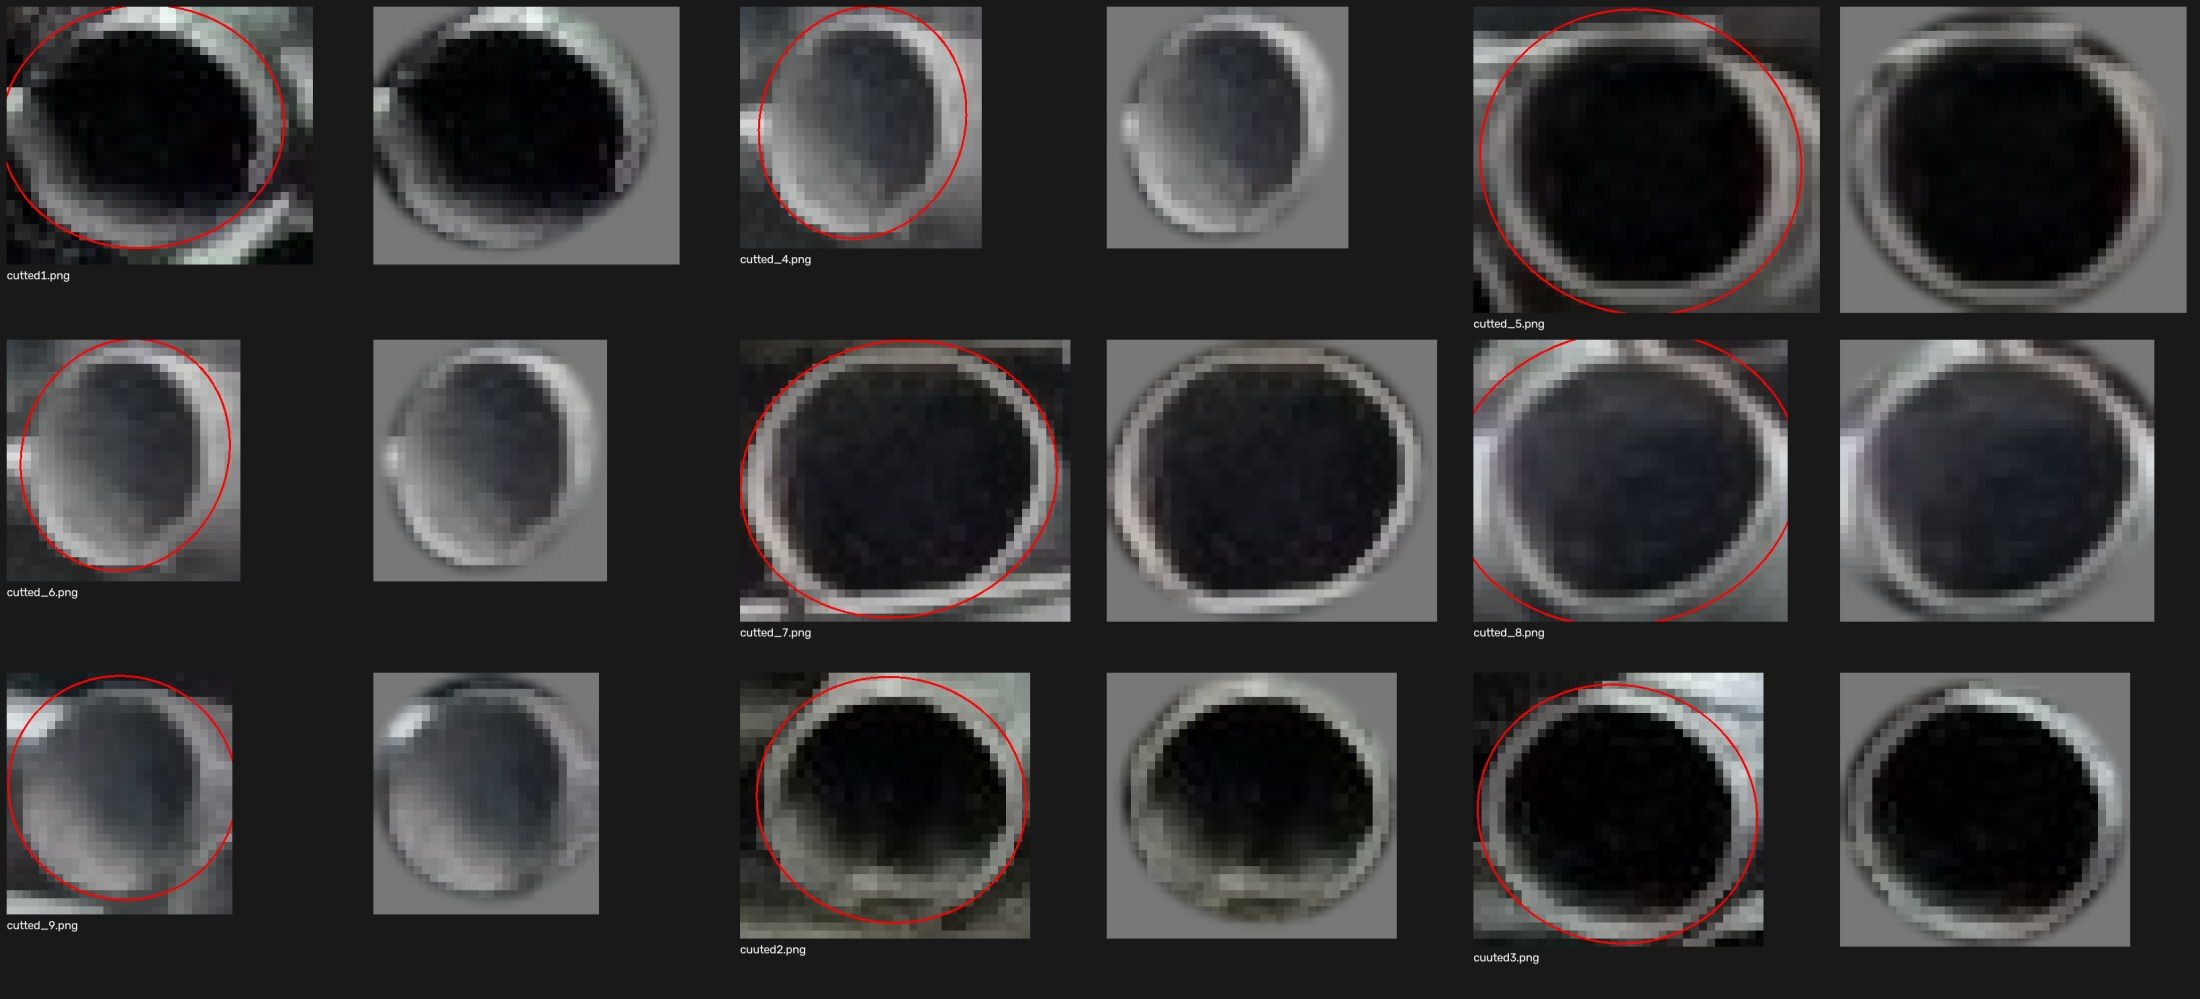
\includegraphics[width=\textwidth]{abbildungen/matting_check.jpg}
\caption[Kontrolle des Freistellens]{Kontrolle des Freistellens für alle neun
Ausschnitte. Je Paar links das Original mit eingezeichneter Ellipse, rechts das
freigestellte Objekt auf neutralem Grau. Erkennbar ist die weiche Kante und der
bewusst außen liegende Maskenrand, der den hellen Kranz vollständig einschließt.}
\label{abb:matting}
\end{figure}

\section{Stufe 2 -- Okkluder-Bibliothek}
\label{sec:okkluderbib}

\absatz{Warum echte Rohrschäfte statt gezeichneter Balken.} Verdeckung liegt in
der Zieldomäne durch quer liegende Rohre vor. Ein synthetisch \emph{gemalter}
Balken hätte andere Textur-, Rausch- und Glanzstatistik als der Rest des Bildes
-- das Netz könnte \enquote{Objekt liegt neben künstlichem Balken} lernen, also
eine Abkürzung der Klasse S2--S4. Die vier Clean Plates sind dagegen buchstäblich
Wände aus Rohrschäften desselben Materials, derselben Kamera und derselben
Beleuchtung. Aus ihnen lassen sich Okkluder gewinnen, deren
Sensorsignatur identisch ist.

\absatz{Verfahren.}
\begin{enumerate}
  \item Bestimmung der dominanten Rohrrichtung über den \textbf{Struktur-Tensor}
  \parencite{jaehne2005}, Winkel auf $(-45^\circ, 45^\circ]$ gefaltet, Bild
  entsprechend gedreht. Gemessen: $+0{,}9^\circ$, $-1{,}6^\circ$,
  $+0{,}9^\circ$, $+6{,}6^\circ$.
  \item Zeilenmittelprofil des gedrehten Bildes, Hochpassfilterung, lokale
  Maxima als \textbf{Rohrachsen}; ihr mittlerer Abstand ist der Rohrdurchmesser.
  Gemessen: 16, 18, 21, 20\px{} -- dieselben Werte, die
  Tabelle~\ref{tab:hintergruende} als Maßstabsanker nennt.
  \item Ausschneiden eines Streifens der Höhe = Achsabstand um jede Achse.
  \item Weiche \textbf{Kapselmaske} (Rechteck mit halbrunden Enden, 1,6\px{}
  Feder), damit die Schaftenden nicht als gerade Schnittkante enden.
\end{enumerate}

\absatz{Ergebnis.} 56 Rohrschäfte mit echter zylindrischer Schattierung und
echtem Glanzlicht (Abbildung~\ref{abb:okkluder}). Sie werden in der Synthese
zweifach verwendet: als Schaft \emph{hinter} jeder Stirnfläche
(Abschnitt~\ref{sec:schaft}) und als quer liegender Okkluder \emph{vor} dem
Stapel (Abschnitt~\ref{sec:okklusion}).

\begin{figure}[htbp]
\centering
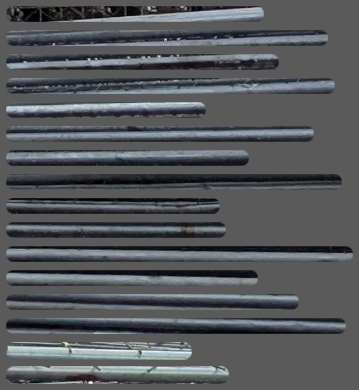
\includegraphics[width=0.42\textwidth]{abbildungen/okkluder_check.png}
\caption[Okkluder-Bibliothek]{Ausschnitt aus der Okkluder-Bibliothek: aus den
Clean Plates extrahierte echte Rohrschäfte mit zylindrischer Schattierung,
Glanzlicht und weicher Kapselmaske.}
\label{abb:okkluder}
\end{figure}

\section{Stufe 3 -- Bildsynthese}
\label{sec:synthese}

Die Leinwand ist $1024\times1024$ Pixel groß und damit identisch zur
Trainingsauflösung \code{imgsz=1024}. Das ist eine bewusste Entscheidung nach
Anforderung~A2: Die synthetischen Bilder durchlaufen im Training \emph{keine}
Größenänderung, die sorgfältig kalibrierte Objektgrößenverteilung bleibt exakt
erhalten.

\subsection{T1 -- Hintergrund}
\label{sec:hintergrundstufe}

\begin{table}[htbp]
\centering
\caption[T1: Hintergrundstufe]{T1 -- Hintergrundstufe. \emph{Ist} = gemessener
Anteil je Bild im erzeugten Datensatz. Belegart wie in
Tabelle~\ref{tab:mapping}.}
\label{tab:t1}
\footnotesize
\begin{tabularx}{\textwidth}{@{}L{0.20\textwidth}L{0.10\textwidth}XL{0.045\textwidth}@{}}
\toprule
\textbf{Transformation} & \textbf{Ist} & \textbf{Begründung} & \textbf{Art} \\
\midrule
Clean Plate statt Fremdszene & 80\,\% (Soll) &
Die vier Clean Plates sind exakt die Zieldomäne und erhalten sechsfaches
Ziehgewicht. Die drei Fremdszenen liefern zu 20\,\% Kontextvielfalt und harte
Negative -- \code{bg\_5.jpg} enthält den Maschendraht, der nach der
Annotationsdefinition kein Objekt ist. & M \\
Zoom gekoppelt an den Rohrdurchmesser & 100\,\% &
\textbf{Physikalische Randbedingung} (Befund~6). Statt Zoom und Objektgröße
unabhängig zu ziehen, gilt $d = d_{\text{Rohr}}(\text{bg}) \cdot z$. Ein
Missverhältnis zwischen Stirnfläche und benachbartem Schaft wäre physikalisch
unmöglich und trainierte eine falsche Kontext-Größen-Relation an. & P \\
Zufallsausschnitt (Translation) & 100\,\% &
Verhindert, dass immer derselbe Bildbereich als Hintergrund dient -- bei nur
sieben Quellbildern die wichtigste Quelle von Hintergrundvielfalt. & L \\
Reflect-Padding statt Kachelung & nach Bedarf &
Wird der geforderte Ausschnitt größer als das Quellbild, so wird gespiegelt
aufgefüllt, gedeckelt auf $1{,}35 \times$ kürzeste Kante. \code{np.tile} erzeugte
harte achsparallele Nähte (S1); gespiegeltes Padding hat keine Kante. & L \\
Horizontale Spiegelung & 50{,}5\,\% &
Label-exakt und physikalisch korrekt: Ein Stapel wird von beiden Enden
fotografiert. & P \\
Vertikale Spiegelung & 14{,}9\,\% &
Ebenfalls label-exakt. Bewusst seltener als horizontal, weil die Schwerkraft
(Stapel unten, Himmel oben) eine schwache Vorzugsrichtung erzeugt. & A \\
Kleinrotation $\pm 6^\circ$ & 34{,}3\,\% &
Die Rohrlinien im Bild sind nie exakt achsparallel; ohne diese Variation wäre
die Vorzugsrichtung im Datensatz künstlich diskret. Angewandt \emph{vor} dem
Einfügen der Objekte, betrifft also keine Boxen. Begleitender Zoom 1,06 gegen
Eckartefakte. & M \\
\bottomrule
\end{tabularx}
\end{table}

Der Zoomfaktor $z$ wird so gezogen, dass der resultierende Basisdurchmesser im
Zielbereich $[d_{\min}, d_{\max}] = [12, 44]$\px{} liegt:
\begin{equation}
z \sim \mathcal{U}\!\left[\;\max\!\left(0{,}55,\;
\frac{d_{\min}}{d_{\text{Rohr}}}\right),\;
\min\!\left(2{,}20,\;\frac{d_{\max}}{d_{\text{Rohr}}}\right)\right],
\qquad d_{\text{Basis}} = d_{\text{Rohr}} \cdot z .
\label{eq:zoom}
\end{equation}
Die äußeren Schranken 0,55 und 2,20 begrenzen die Vergrößerung des
Hintergrundmaterials und damit den Verlust an Hintergrundschärfe. Für
$d_{\text{Rohr}} = 16$\px{} ergibt Gleichung~\eqref{eq:zoom}
$z \in [0{,}75;\,2{,}20]$, für $d_{\text{Rohr}} = 21$\px{}
$z \in [0{,}57;\,2{,}10]$. Der Ausschnitt der Kantenlänge $1024/z$ wird
anschließend auf die Leinwand skaliert -- beim Verkleinern flächentreu
(\code{INTER\_AREA}), um Aliasing zu vermeiden (S3).

\subsection{T2 -- Geometrie der Einzelinstanz}
\label{sec:instanzgeometrie}

\begin{table}[htbp]
\centering
\caption[T2: Instanzgeometrie]{T2 -- Geometrie der Einzelinstanz. \emph{Ist} =
gemessener Anteil je gerenderter Instanz.}
\label{tab:t2}
\footnotesize
\begin{tabularx}{\textwidth}{@{}L{0.19\textwidth}L{0.11\textwidth}XL{0.045\textwidth}@{}}
\toprule
\textbf{Transformation} & \textbf{Ist} & \textbf{Begründung} & \textbf{Art} \\
\midrule
Rotation $0$--$360^\circ$ & 100\,\% &
Rohrenden haben keine kanonische Bildorientierung: Kamerarollwinkel und
Stapelausrichtung sind beliebig. Die einzige Orientierungsinformation ist die
Richtung des Glanzlichts auf dem Kranz, und die hängt vom Sonnenstand ab. Volle
Rotationsinvarianz ist daher korrekt \emph{und kostenlos} -- es gibt keine
Rotation, die ein unmögliches Bild erzeugt. Deshalb 100\,\% statt eines
Bruchteils. & P \\
Skalierung auf 12--44\px{} & 100\,\% &
Reale Messung (Tabelle~\ref{tab:objektstatistik}): \code{val} 20,6--35,8\px{},
\code{test} 12,2--31,9\px{}. Der Generator deckt die reale Spanne plus rund
25\,\% Reserve nach oben ab, für Aufnahmen aus geringerem Abstand.
Ist-Verteilung im Datensatz: p05 11,6 / Median 22,5 / p95 39,9\px{}.
Verkleinerung flächentreu, weil bilineare Interpolation Aliasing als
verräterisches Hochfrequenzmuster im Objekt zurückließe (S3). & M \\
Ovalisierung & 57{,}1\,\% &
Reale Messung: Seitenverhältnis p10--p90 = 0,97--1,31 (\code{val}) bzw.\
0,85--1,22 (\code{test}); über die Hälfte der echten Boxen weicht um
$\geq 5\,\%$ vom Quadrat ab. Zwei physikalische Ursachen: Schrägansicht
projiziert den Kreis auf eine Ellipse, und Rohre sind tatsächlich gequetscht.
Der Anteil bildet die gemessene Häufigkeit ab. Aufteilung 45\,\% oblat
(0,66--0,97) zu 12\,\% prolat (1,03--1,30), weil Schrägansicht die Höhe
verkürzt und häufiger ist als eine seitliche Quetschung. & M \\
Delle & 18{,}1\,\% &
Modelliert mechanisch beschädigte Rohrenden. \textbf{Der Anteil ist eine
Annahme, keine Messung} -- Dellen sind in \code{val}/\code{test} nicht separat
annotiert. 18\,\% wurde gewählt, damit das Modell die Verformung regelmäßig
sieht (etwa jedes fünfte Objekt, im Mittel vier pro Bild), sie aber die
Formstatistik nicht dominiert. Ein zu hoher Anteil würde die Rundheit als
Merkmal verwässern und Falschpositive auf beliebigen dunklen Flecken erzeugen
(vgl.\ Abschnitt~\ref{sec:auggrenzen}). & A \\
Perspektive & 30{,}2\,\% &
Bei Schrägblick wird der Kreisring nicht nur zur Ellipse -- der helle Kranz wird
auf einer Seite auch \emph{breiter}, weil die Rohrinnenwand sichtbar wird. Eine
rein anisotrope Skalierung kann das nicht abbilden. Der Anteil ist eine Annahme;
30\,\% spiegelt die Beobachtung, dass in \code{val}/\code{test} die Mehrheit der
Stirnflächen annähernd frontal steht. & A \\
\bottomrule
\end{tabularx}
\end{table}

\absatz{Skalierung und Ovalisierung.} Beide werden in einem Schritt ausgeführt.
Ist $d_{\text{src}}$ der Durchmesser des Quellausschnitts, $d$ der Zieldurchmesser
und $\rho$ das gezogene Achsverhältnis, so gilt
\begin{equation}
s_x = \frac{d}{d_{\text{src}}\sqrt{\rho}}, \qquad
s_y = \frac{d\,\sqrt{\rho}}{d_{\text{src}}} .
\label{eq:oval}
\end{equation}
Der geometrische Mittelwert bleibt dabei erhalten:
$\sqrt{s_x s_y}\, d_{\text{src}} = d$. Das ist kein Zufall, sondern notwendig,
damit die Ovalisierung die kalibrierte Größenverteilung nicht verschiebt -- die
Realmessung in Tabelle~\ref{tab:objektstatistik} verwendet mit
$\sqrt{\text{Fläche}}$ genau dieses Maß.

\absatz{Dellenmodell.} Die Einbeulung wird als glatte radiale Verschiebung
umgesetzt. Für $K \in \{1,2\}$ Winkelsektoren mit Mittelrichtungen $\varphi_k$,
Breiten $\sigma_k \sim \mathcal{U}[0{,}30;\,0{,}85]$\,rad und
Eindringtiefen $a_k \sim \mathcal{U}[0{,}10;\,0{,}30]$ lautet das
Verschiebungsfeld in Polarkoordinaten um den Objektmittelpunkt
\begin{equation}
u(r, \varphi) = \sum_{k=1}^{K} a_k
\exp\!\left(-\left(\frac{\Delta\varphi_k}{\sigma_k}\right)^{2}\right)
\left(\frac{r}{R}\right)^{2},
\qquad \Delta\varphi_k = \operatorname{atan2}\!\big(\sin(\varphi-\varphi_k),
\cos(\varphi-\varphi_k)\big),
\label{eq:delle}
\end{equation}
und die Abtastung erfolgt an $r \cdot (1 + u)$. Die quadratische Radiusgewichtung
$(r/R)^2$ ist der wesentliche Modellierungsentscheid: Sie hält das Zentrum ruhig
und verformt nur den Rand. Eine gleichmäßige Verschiebung würde die dunkle
Bohrung mitverzerren und damit das Merkmalspaar Kranz/Bohrung zerstören, statt
nur den Umriss zu beschädigen.

\absatz{Perspektive.} Umgesetzt als milde Homographie: Die vier Eckpunkte des
Instanzausschnitts werden unabhängig um bis zu $\pm 9\,\%$ der Kantenlänge
verschoben. Der Wert 9\,\% ist so gewählt, dass die entstehende Verzerrung
sichtbar, aber nicht mit einer Schrägansicht von mehr als etwa $25^\circ$
verwechselbar ist -- stärkere Verzerrungen kämen bei einer frontal auf den
Stapel gerichteten Kamera nicht vor.

\absatz{Rotation.} Die Instanz wird auf eine quadratische Leinwand der Größe
ihrer Diagonale erweitert und um $\theta \sim \mathcal{U}[0^\circ, 360^\circ]$
gedreht. Die Box wird anschließend nicht aus $\theta$ berechnet, sondern aus der
gedrehten Alphamaske selbst -- damit entfällt die in
Abschnitt~\ref{sec:boxrotation} beschriebene Aufblähung vollständig
(Anforderung~A1).

\subsection{T3 -- Photometrie und Einbettungsrealismus}
\label{sec:photometrie}

Diese Stufe schließt die Signaturen S2--S4 und S6. Sie ist der aufwendigste Teil
der Pipeline und derjenige, dessen Wirkung optisch am wenigsten auffällt.

\begin{table}[htbp]
\centering
\caption[T3: Photometrie und Einbettungsrealismus]{T3 -- Photometrie der
Einzelinstanz und Einbettungsrealismus. \emph{Ist} = gemessener Anteil je
gerenderter Instanz. Die Spalte \emph{S} nennt die geschlossene Abkürzung aus
Abschnitt~\ref{sec:shortcut}.}
\label{tab:t3}
\footnotesize
\begin{tabularx}{\textwidth}{@{}L{0.19\textwidth}L{0.07\textwidth}L{0.035\textwidth}XL{0.045\textwidth}@{}}
\toprule
\textbf{Transformation} & \textbf{Ist} & \textbf{S} & \textbf{Begründung} & \textbf{Art} \\
\midrule
Helligkeit $\times 0{,}70$--$1{,}35$ & 99{,}8\,\% & -- &
Stirnflächen liegen je nach Stapelposition in praller Sonne oder tiefem
Schatten. Die Spannweite ist aus den Ausschnitten selbst ablesbar: mittlere
Kranzhelligkeit 88--156 Grauwerte. Praktisch 100\,\%, weil es keine
\enquote{richtige} Helligkeit gibt, die bevorzugt werden dürfte. & M \\
Gamma $0{,}75$--$1{,}35$ & 79{,}7\,\% & -- &
Gamma statt reinem Kontrast, weil es die nichtlineare Tonwertkurve
unterschiedlicher Kameras und JPEG-Pipelines abbildet
\parencite{grossberg2003}. Es verändert vor allem das Verhältnis dunkle Bohrung
$\leftrightarrow$ heller Kranz -- genau das Merkmal, auf das der Detektor sonst
zu starr konditioniert würde. & L \\
HSV (Ton $\pm 8^\circ$, Sättigung $\times 0{,}45$--$1{,}60$) & 69{,}7\,\% & -- &
Verzinkter Stahl ist nahezu neutralgrau, nimmt aber Farbstiche an: Flugrost
braun, Moos grün, blauer Himmel als Reflex. Der Farbtonhub ist bewusst klein --
große Sprünge wären unphysikalisch. & M \\
Farbangleich an den lokalen Hintergrund & 84{,}8\,\% & S2 &
\textbf{Die wichtigste Anti-Abkürzungs-Maßnahme.} Ausschnitt und Hintergrund
stammen aus verschiedenen Aufnahmen mit verschiedenem Weißabgleich und
Belichtungsniveau; ohne Angleich bleibt ein konstanter Versatz, den ein CNN
trivial als Einfügemarke lernt. Bewusst nur \emph{teilweise}
(Gleichung~\eqref{eq:harmonize}). & L \\
Unschärfeangleich ($\sigma$ 0,25--1,10\px) & 59{,}8\,\% & S3 &
Zwei Gründe: Das skalierte Objekt ist je nach Skalierungsrichtung glatter oder
schärfer als das Zielbild, und reale Objekte liegen je nach Stapeltiefe
außerhalb der Schärfeebene. Schärfe ist eine der beiden Sensorsignaturen, an
denen eingeklebte Pixel am leichtesten erkennbar sind
\parencite{popescu2005}. & L \\
Rauschangleich ($\times 0{,}5$--$1{,}25$ der lokalen Schätzung) & 69{,}9\,\% & S4 &
Die zweite Sensorsignatur \parencite{lukas2006}. Beim Verkleinern eines
Ausschnitts sinkt dessen Rauschen; der eingeklebte Bereich wäre dann messbar
sauberer als seine Umgebung. Das Rauschniveau wird \emph{pro Einfügestelle
gemessen} (Gleichung~\eqref{eq:noise}), nicht global gesetzt -- die Hintergründe
liegen zwischen 6,8 und 15,2 Grauwerten Hochpassstreuung. & L \\
Alphakante weichzeichnen ($\sigma$ 0,4--1,0\px) & 100\,\% & S1 &
Immer. Eine pixelharte Silhouette gibt es bei 25\px{}-Objekten in echten
Aufnahmen nicht. & P \\
Schlagschatten & 49{,}3\,\% & S6 &
Ohne Kontaktschatten \enquote{schwebt} ein eingeklebtes Objekt sichtbar. Rund
50\,\%, weil bei diffusem Licht -- alle vier Clean Plates sind bedeckt
aufgenommen -- etwa die Hälfte der realen Objekte keinen sichtbaren
Schlagschatten wirft. & A \\
\bottomrule
\end{tabularx}
\end{table}

\absatz{Farbangleich.} Umgesetzt als \emph{partieller} Statistiktransfer im Stil
des Farbtransfers von \textcite{reinhard2001}. Für jeden Farbkanal $c$ seien
$\mu_i, \sigma_i$ Mittelwert und Streuung der Objektpixel (Alphamaske $> 0{,}5$)
und $\mu_b, \sigma_b$ dieselben Größen des lokalen Hintergrundausschnitts. Dann
gilt
\begin{equation}
c' = \mu_i + k\,(c - \mu_i) + \alpha_\mu\,(\mu_b - \mu_i),
\qquad
k = 1 + \alpha_\sigma\left(\operatorname{clip}\!\left(
\frac{\sigma_b}{\sigma_i},\, 0{,}6,\, 1{,}6\right) - 1\right)
\label{eq:harmonize}
\end{equation}
mit $\alpha_\mu \sim \mathcal{U}[0{,}10;\,0{,}45]$ und
$\alpha_\sigma \sim \mathcal{U}[0;\,0{,}35]$. Für
$\alpha_\mu = \alpha_\sigma = 1$ ginge Gleichung~\eqref{eq:harmonize} in den
vollständigen Reinhard-Transfer über. Genau das ist hier \emph{nicht} gewollt:
Ein vollständiger Angleich würde den intrinsischen Albedo-Unterschied zwischen
dunkler Bohrung und hellem Kranz einebnen und damit das Objekt zerstören.
Modelliert wird also ausschließlich die \emph{Beleuchtungs- und
Weißabgleichdifferenz} zwischen den Aufnahmen, nicht die Objektfarbe. Die
Klemmung des Streuungsverhältnisses auf $[0{,}6;\,1{,}6]$ verhindert
Ausreißer an Einfügestellen mit sehr homogenem Hintergrund, wo
$\sigma_b/\sigma_i$ beliebig klein werden kann.

\absatz{Rauschschätzung.} Das lokale Rauschniveau wird als Streuung eines
Hochpassrests geschätzt -- ein Verfahren in der Tradition von
\textcite{immerkaer1996}, hier mit einem Medianfilter als Tiefpass, weil er
Kanten weniger verschmiert als ein Gaußkern:
\begin{equation}
\hat{\sigma} = \operatorname{std}\!\big(g - \operatorname{median}_{3\times3}(g)\big),
\qquad
\sigma_{\text{Rausch}} = \max\big(0{,}5,\; \hat{\sigma} \cdot
\mathcal{U}[0{,}5;\,1{,}25]\big).
\label{eq:noise}
\end{equation}
Die Multiplikation mit einem Faktor um 1 statt der direkten Verwendung von
$\hat\sigma$ ist Absicht: Die Schätzung enthält neben dem Rauschen auch
Texturanteile und überschätzt das Niveau an strukturreichen Stellen.

\absatz{Schlagschatten.} Die Alphamaske wird mit $\sigma = 0{,}10 \cdot
\max(h,w)$ geglättet, um $\Delta x \sim \mathcal{U}[-0{,}22;\,0{,}22]\,w$ und
$\Delta y \sim \mathcal{U}[0{,}02;\,0{,}26]\,h$ verschoben und die Leinwand dort
um den Faktor $1 - \kappa\,s$ mit $\kappa \sim \mathcal{U}[0{,}18;\,0{,}45]$
abgedunkelt. Der Versatz ist in $y$ ausschließlich positiv: Bei einer von unten
oder frontal aufgenommenen Szene mit Himmelslicht fällt der Kontaktschatten nach
unten.

\subsection{T4 -- Layout}
\label{sec:layout}

Das Layoutmodell ist eine \textbf{gescherte, verrauschte Gitterpackung} je
Cluster. Pro Bild werden 1--3 Cluster gezogen (Anteile 45/35/20\,\%), dazu 0--3
vereinzelte Profile. Innerhalb eines Clusters mit Basisdurchmesser $d_0$ liegen
die Zentren auf
\begin{equation}
p_{ij} = i\,s_1\,\mathbf{e}_1 + j\,s_2\,\mathbf{e}_2 + \mathbf{c}
+ \boldsymbol{\epsilon}_{ij},
\qquad \boldsymbol{\epsilon}_{ij} \sim \mathcal{N}(\mathbf{0},
(0{,}17\,d_0)^2 \mathbf{I}),
\label{eq:layout}
\end{equation}
mit $i = 0,\dots,n_1{-}1$, $j = 0,\dots,n_2{-}1$,
$n_1 \in \{2,\dots,13\}$, $n_2 \in \{1,\dots,6\}$, Gitterabständen
$s_1 \sim \mathcal{U}[0{,}98;\,1{,}60]\,d_0$ und
$s_2 \sim \mathcal{U}[0{,}98;\,1{,}85]\,d_0$ sowie Basisrichtungen
$\mathbf{e}_1, \mathbf{e}_2$, die einen Winkel zwischen $55^\circ$ und
$125^\circ$ einschließen. Die Hauptrichtung liegt mit Wahrscheinlichkeit 0,6 im
Bereich $60$--$150^\circ$, sonst gleichverteilt -- das bildet die in
Tabelle~\ref{tab:anordnung} gemessene leichte Häufung der Nachbarrichtungen ab,
ohne sie zu einer harten Regel zu machen.

Zwei Modellentscheidungen folgen unmittelbar aus den Messungen:

\begin{itemize}
  \item \textbf{Eine Basisgröße pro Cluster}, je Instanz nur
  $\mathcal{U}[0{,}92;\,1{,}09]$ Streuung. Begründung: Befund~8 (gemessenes
  Größenverhältnis benachbarter Objekte im Median 1,05). Jede Instanz unabhängig
  zu würfeln wäre ein sofort sichtbarer Realismusfehler.
  \item \textbf{Das Clusterzentrum darf außerhalb der Leinwand liegen}
  ($\mathbf{c} \sim \mathcal{U}[-0{,}12;\,1{,}12]^2 \cdot 1024$), sodass
  angeschnittene Objekte am Bildrand entstehen. Begründung: In \code{test} sind
  5,8\,\% der Labels angeschnitten.
\end{itemize}

\absatz{Abgedunkelte Mulde.} Zusätzlich wird je Cluster mit Wahrscheinlichkeit
0,55 eine weiche, anisotrope Gaußmulde unter das Cluster gelegt (Radius
$2{,}5$--$7{,}0\,d_0$, Abdunklung 10--38\,\%); gemessen ergibt das im Mittel
0,87 Mulden pro Bild. Begründung: In den echten Aufnahmen liegen die
Stirnflächen am Stapelrand \emph{vor} dem verschatteten Stapelinneren; der
Hintergrund hinter ihnen ist deutlich dunkler als die besonnten Schäfte davor.
Ohne diese Abdunklung stünden die dunklen Bohrungen kontrastmäßig zu isoliert da
-- und wären damit als Gruppe leichter von echten Aufnahmen unterscheidbar.

\subsection{T5 -- Rohrschaft hinter jeder Stirnfläche}
\label{sec:schaft}

Dies ist die wichtigste Einzelentscheidung der Pipeline und ein Musterbeispiel
für Anforderung~A3.

\absatz{Begründung.} Nach Befund~9 gilt in den Realbildern ausnahmslos: Hinter
jeder annotierten Stirnfläche führt ein sichtbarer Rohrschaft weg. Ein dunkler
Kreis mitten auf einem durchgehenden Rohr ist physikalisch unmöglich. Die erste
Generatorversion erzeugte genau das und sah entsprechend falsch aus. Der Generator
setzt daher bei 88,0\,\% der Instanzen einen echten Rohrschaft aus der Bibliothek
von Stufe~2 hinter das Profil.

\begin{table}[htbp]
\centering
\caption[T5: Rohrschaft]{T5 -- Rohrschaft hinter der Stirnfläche.}
\label{tab:t5}
\footnotesize
\begin{tabularx}{\textwidth}{@{}L{0.20\textwidth}L{0.09\textwidth}XL{0.045\textwidth}@{}}
\toprule
\textbf{Parameter} & \textbf{Ist} & \textbf{Begründung} & \textbf{Art} \\
\midrule
Schaft vorhanden & 88{,}0\,\% der Instanzen &
Befund~9. Der Schaft hat exakt den Durchmesser der Stirnfläche
($\times\,0{,}96$--$1{,}06$, dasselbe Rohr), Länge $2$--$24\,\Oe$. Lange Schäfte,
weil in den echten Bildern praktisch jedes Rohr aus dem Ausschnitt herausläuft
oder hinter anderen Rohren verschwindet; kurze Stummel mit sichtbarer runder
Kappe wären ein verräterisches Muster. & P \\
Schaftrichtung je Cluster parallel ($\pm 11^\circ$) & 100\,\% &
Alle Rohre eines Stapels liegen parallel und verkanten nur leicht. Eine
Streuung von $\pm 18^\circ$ erzeugte sichtbar einen sternförmigen Fächer, den es
real nicht gibt. Die Bedingung gilt \emph{innerhalb} eines Clusters; gegen die
Rohrrichtung des Hintergrunds ist sie nicht erzwungen
(Abschnitt~\ref{sec:grenzen}). & P \\
Helligkeitsangleich an die Umgebung & 100\,\% &
Die Schaftbibliothek stammt aus vier Aufnahmen mit stark unterschiedlichem
Belichtungsniveau (Hintergrundmittel 70--102 Grauwerte). Ohne Angleich
($\kappa = 0{,}35$--$0{,}75$ des Differenzmittels) klebten sichtbar zu dunkle
Rohre im Bild. & M \\
75\,\% der Schäfte ganz hinten, 25\,\% eingereiht & -- &
\textbf{Tiefenmodell}, siehe unten. & M \\
\bottomrule
\end{tabularx}
\end{table}

\absatz{Das Tiefenmodell und wie es gefunden wurde.} Die Stirnflächen eines
Stapels bilden eine Front; die zugehörigen Schäfte laufen von dieser Front
\emph{weg} und liegen in der Projektion daher hinter allen Stirnflächen. Nur
Rohre, die quer vor dem Stapel liegen, kreuzen vor anderen Enden -- in
\code{val}/\code{test} sichtbar, aber die Minderheit.

Bemerkenswert ist, wie dieser Modellparameter bestimmt wurde: nicht durch
Anschauung, sondern über eine Messung an der erzeugten Verteilung. Mit rein
zufälliger Tiefenordnung verdeckten die Schäfte so viele Nachbarn, dass deren
Labels nach der Sichtbarkeitsregel wegfielen; der mittlere Abstand zum nächsten
Nachbarn im synthetischen Datensatz stieg dadurch auf $1{,}55\,\Oe$ -- rund
40\,\% über dem real gemessenen Wert von $1{,}09$--$1{,}24\,\Oe$. Mit dem
75/25-Modell liegt er bei $1{,}17\,\Oe$. Der Parameter ist damit an einer
Realmessung kalibriert, nicht geschätzt. Dieses Vorgehen -- eine erzeugte
Statistik gegen die gemessene Statistik zu prüfen und den Generator daraufhin zu
korrigieren -- ist die einzige Möglichkeit, den Divergenzterm
$d_{\mathcal{H}\Delta\mathcal{H}}$ aus Gleichung~\eqref{eq:bendavid} ohne
zusätzliche Trainingsläufe zu senken.

\subsection{T6 -- Okklusion}
\label{sec:okklusion}

Verdeckung entsteht in der Pipeline aus \emph{vier} verschiedenen, jeweils
physikalisch motivierten Quellen. Der Unterschied zu generischen
Okklusionsverfahren wie Cutout \parencite{devries2017cutout} oder Random Erasing
\parencite{zhong2020erasing} ist wesentlich: Dort wird Bildinhalt gelöscht, das
Label aber unverändert gelassen. Hier verdeckt ein \emph{Objekt} mit eigener
Textur, und die Sichtbarkeit wird berechnet und in die Labelentscheidung
überführt (Abschnitt~\ref{sec:sichtbarkeit}). Das erzeugt nicht nur schwierigere
positive Beispiele, sondern auch korrekte harte Negative.

\begin{table}[htbp]
\centering
\caption[T6: Okklusionsquellen]{T6 -- die vier Okklusionsquellen.}
\label{tab:t6}
\footnotesize
\begin{tabularx}{\textwidth}{@{}L{0.20\textwidth}L{0.13\textwidth}XL{0.045\textwidth}@{}}
\toprule
\textbf{Quelle} & \textbf{Ist} & \textbf{Begründung} & \textbf{Art} \\
\midrule
Andere Profile & intrinsisch &
Bei einem NN-Abstand von $0{,}84\,\Oe$ im 10.\ Perzentil überlappen benachbarte
Stirnflächen zwangsläufig. Die Tiefenordnung ist zufällig, das
Verdeckungsverhältnis damit unverzerrt. & M \\
Echte Rohrschäfte quer davor & 58{,}4\,\% der Bilder, 1--6 Stück &
Rohre, die vor dem Stapel liegen. Breite $0{,}55$--$1{,}35\,\Oe$, Länge
$4$--$26 \times$ Breite; zu 80\,\% bevorzugt durch ein Cluster gelegt statt ins
Leere, weil eine Verdeckung, die kein Objekt trifft, keinen Trainingsnutzen hat. & M \\
Eigene Schäfte (die eingereihten 25\,\%) & s.\ T5 &
Physikalisch der häufigste Verdeckungsfall in den Realbildern. & P \\
Fremdkörper (Laub, Draht, Schnee) & 31{,}6\,\% der Bilder, 1--4 Stück &
Aus den Hintergründen selbst geschnitten, mit unregelmäßiger weicher Maske aus
geglättetem Rauschen. Dass sie aus demselben Material stammen, schließt
Signatur~S4 auch für die Okkluder. In \code{test4\_cutted.png} liegt reichlich
Laub auf dem Stapel. & M \\
Bildrand & $\approx 3\,\%$ der Objekte & siehe T4. & M \\
\bottomrule
\end{tabularx}
\end{table}

\absatz{Ergebnis.} 30,1\,\% aller gelabelten Objekte sind teilverdeckt
(Sichtbarkeit $< 95\,\%$); die mittlere Sichtbarkeit der gelabelten Objekte
beträgt 90,0\,\%. Über alle gerenderten Instanzen -- also einschließlich der
verworfenen -- liegt sie bei 75,7\,\%.

\subsection{T7 -- Sichtbarkeitsrechnung und Labelerzeugung}
\label{sec:sichtbarkeit}

Kein Copy-Paste-Generator darf Labels blind vergeben: Ein Objekt, das nach dem
Einfügen zu 95\,\% verdeckt ist, hat kein sinnvolles Label mehr. Für \emph{jede}
Instanz wird daher die exakte Sichtbarkeit berechnet. Grundlage ist die
Alpha-Kompositionsregel von \textcite{porter1984}: Wird die Instanz $i$ vor allen
später gemalten Schichten $j$ überlagert, so ist der verbleibende sichtbare
Anteil ihrer Alphamaske
\begin{equation}
\alpha_i^{\text{sichtbar}} = \alpha_i \prod_{j > i} \big(1 - \alpha_j\big),
\qquad
v_i = \frac{\sum \alpha_i^{\text{sichtbar}}}{\sum \alpha_i},
\label{eq:sichtbarkeit}
\end{equation}
wobei das Produkt über \emph{alle} nach $i$ gemalten Schichten läuft --
einschließlich anderer Profile, Rohrschäfte und Fremdkörper. Die Buchhaltung
läuft über die beschnittenen Alphafenster in Malreihenfolge, ist also exakt und
nicht approximiert.

\begin{table}[htbp]
\centering
\caption[T7: Labelregeln]{T7 -- Regeln der Labelerzeugung mit den absoluten
Zahlen des erzeugten Datensatzes (6000 Bilder, 173\,100 gerenderte Instanzen).}
\label{tab:t7}
\footnotesize
\begin{tabularx}{\textwidth}{@{}L{0.22\textwidth}L{0.14\textwidth}X@{}}
\toprule
\textbf{Regel} & \textbf{betroffen} & \textbf{Begründung} \\
\midrule
Label verwerfen, wenn $v_i < 0{,}30$ &
30\,801 Objekte (17{,}8\,\% der gerenderten) &
Unter 30\,\% sichtbarer Fläche wäre das Objekt auch für einen menschlichen
Annotator nicht mehr sicher als Rohrende identifizierbar. Ein Label hier zwingt
das Netz zum Halluzinieren; \emph{kein} Label macht dieselbe Bildstelle zum
korrekten harten Negativ. Es ist dieselbe Regel, nach der \code{val} und
\code{test} annotiert wurden (Anforderung~A5). \\
Label verwerfen, wenn $< 15\,\%$ der Fläche im Bild liegt &
3\,846 Objekte &
Ein Splitter am Bildrand wird real nicht annotiert. Nicht mehr als 15\,\%, weil
\code{test} sehr wohl stark angeschnittene Objekte enthält (kleinste Box:
0,7\,\% der Bildhöhe). \\
Label verwerfen, wenn sichtbare Box $< 5$\px{} &
228 Objekte &
Unterhalb der Auflösungsgrenze; nach Gleichung~\eqref{eq:deff} und Stride~8
nicht mehr lokalisierbar. \\
Modale statt amodale Box & -- &
Genau so wurden \code{val} und \code{test} annotiert
(Abschnitt~\ref{sec:annotation}). Amodale Boxen erzeugten einen systematischen
Größenversatz gegenüber der Ground Truth. \\
\bottomrule
\end{tabularx}
\end{table}

Insgesamt werden 34\,875 der 173\,100 gerenderten Instanzen verworfen
(20,1\,\%). Diese Zahl ist kein Verlust, sondern der eigentliche Ertrag der
Stufe: Sie markiert genau jene Bildstellen, an denen ein naiver Generator ein
falsches Label gesetzt hätte.

\begin{figure}[htbp]
\centering
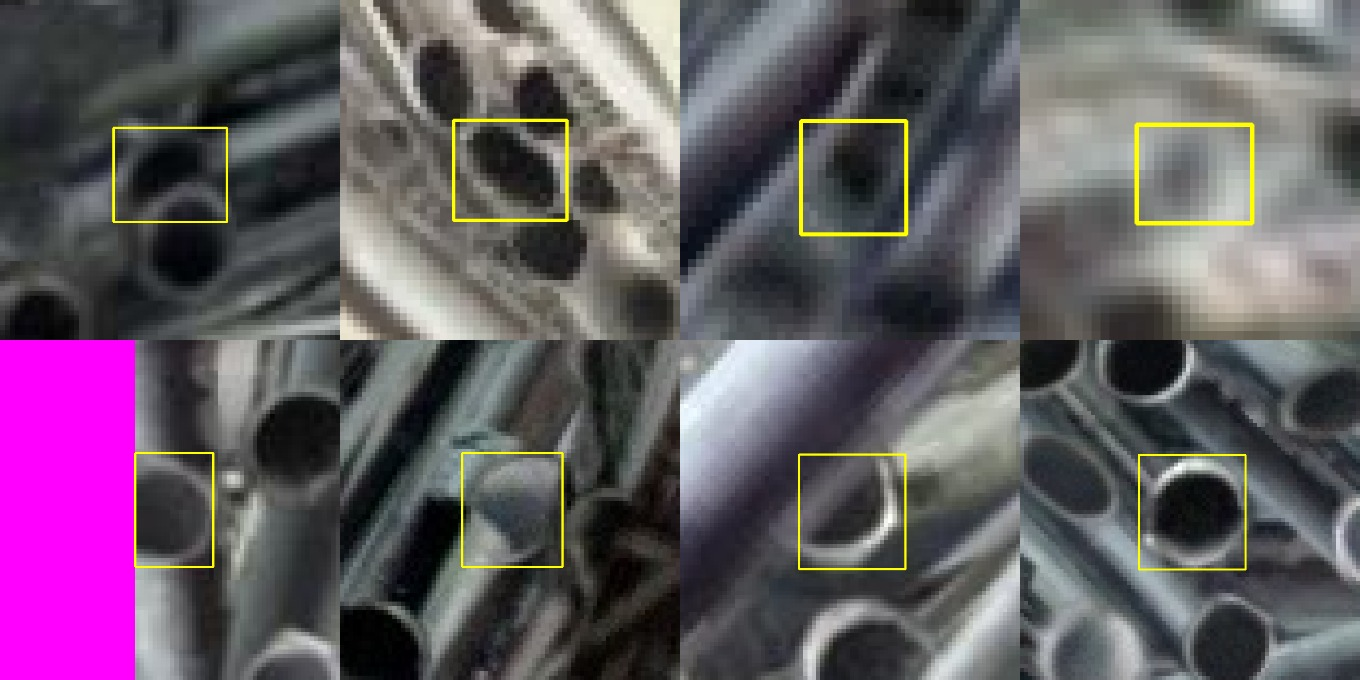
\includegraphics[width=\textwidth]{abbildungen/label_check.jpg}
\caption[Kontrolle der Labelerzeugung]{Kontrolle der Labelerzeugung. Die Boxen
umschließen den \emph{sichtbaren} Umriss; stark verdeckte Instanzen erhalten
kein Label und bleiben damit als hartes Negativ im Bild.}
\label{abb:labelcheck}
\end{figure}

\subsection{T8 -- Globale Bildstufe}
\label{sec:globalstufe}

Die letzte Stufe wirkt auf das \emph{gesamte} Bild. Das ist entscheidend: Nur
eine bildweite Operation kann eine Signatur vereinheitlichen, die zwischen
Objekt und Hintergrund unterscheidbar wäre.

\begin{table}[htbp]
\centering
\caption[T8: Globale Bildstufe]{T8 -- globale Bildstufe. \emph{Ist} = gemessener
Anteil je Bild.}
\label{tab:t8}
\footnotesize
\begin{tabularx}{\textwidth}{@{}L{0.20\textwidth}L{0.07\textwidth}XL{0.045\textwidth}@{}}
\toprule
\textbf{Transformation} & \textbf{Ist} & \textbf{Begründung} & \textbf{Art} \\
\midrule
Helligkeit/Kontrast & 89{,}6\,\% &
Wetter- und Belichtungsvariation ($\times 0{,}80$--$1{,}22$, Offset
$\pm 18$ Grauwerte). & M \\
HSV / Farbtemperatur & 69{,}0\,\% &
Bewölkt (blaustichig) bis Abendsonne (warm). Alle vier Clean Plates sind bei
diffusem Licht aufgenommen -- diese Stufe ist der einzige Ersatz für die
fehlende Beleuchtungsvielfalt und damit eine bewusste Approximation. & A \\
Defokus ($\sigma$ 0,3--1,0\px) & 34{,}4\,\% &
Der Autofokus trifft bei Stapelaufnahmen oft die falsche Ebene. & L \\
Bewegungsunschärfe & 9{,}9\,\% &
Verwacklung aus der Hand; Baustellenaufnahmen entstehen im Vorbeigehen.
Niedriger Anteil, weil moderne Mobiltelefone kurz belichten. & A \\
Sensorrauschen & 80{,}1\,\% &
Vereinheitlicht das Rauschniveau über das ganze Bild
($\sigma = 1{,}0$--$5{,}0$). & L \\
Vignettierung & 25{,}0\,\% &
Weitwinkelobjektive von Mobiltelefonen; erzwingt zusätzlich
Positionsinvarianz der Helligkeit. & L \\
JPEG-Requantisierung $q \in [55, 95]$ & 85\,\% (Soll) &
\textbf{Die wichtigste unsichtbare Transformation} (Signatur~S5). Eingeklebte
Pixel behalten sonst eine andere DCT-Blockstatistik als der Hintergrund, der
bereits einmal komprimiert war \parencite{wallace1992jpeg}. Ein erneuter
Kompressionsdurchlauf über das Gesamtbild vereinheitlicht diese Signatur. Sie
ist forensisch die belastbarste Einfügemarke überhaupt \parencite{farid2009} --
wer sie stehen lässt, liefert dem Netz eine perfekte Abkürzung. & L \\
\bottomrule
\end{tabularx}
\end{table}

\subsection{T9 -- Negativbilder}
\label{sec:negative}

9,7\,\% der erzeugten Bilder enthalten \emph{kein} Objekt: Rohrstapel ohne
Stirnflächen, Kieswerk, Betondeck mit Maschendrahtzaun.

Die Begründung folgt direkt aus der Annotationsdefinition
(Abschnitt~\ref{sec:annotation}): Die dominante Falschpositiv-Quelle in dieser
Domäne sind Rohrschäfte, Gitterknoten und dunkle Löcher im Maschendraht -- alles
Strukturen, die den Stirnflächen ähneln, aber ausdrücklich keine Objekte sind.
Explizite Negativbilder bestrafen genau diese Verwechslung; sie sind das
statische Gegenstück zum Hard-Example-Mining
\parencite{shrivastava2016}. Der Anteil von rund 10\,\% entspricht der Empfehlung
der verwendeten Werkzeugkette \parencite{ultralyticsdocs}; ein höherer Anteil
würde den Anteil positiver Gradienten unnötig verdünnen.

\section{Der erzeugte Datensatz}
\label{sec:datensatz}

\begin{table}[htbp]
\centering
\caption[Kenngrößen des erzeugten Datensatzes]{Kenngrößen des erzeugten
Trainingsdatensatzes.}
\label{tab:datensatz}
\small
\begin{tabular}{@{}lr@{}}
\toprule
Bilder ($1024\times1024$) & 6\,000 \\
davon Negativbilder & 583 \quad (9{,}7\,\%) \\
gerenderte Instanzen & 173\,100 \\
\textbf{gelabelte Objekte} & \textbf{136\,384} \quad (22{,}7 pro Bild) \\
verworfen (Verdeckung / Rand / Größe) & 34\,875 \quad (20{,}1\,\%) \\
mittlere Sichtbarkeit der gelabelten Objekte & 90{,}0\,\% \\
teilverdeckte gelabelte Objekte & 30{,}1\,\% \\
Objektdurchmesser p05 / Median / p95 & 11{,}6 / 22{,}5 / 39{,}9\px \\
Seitenverhältnis p10 / Median / p90 & 0{,}77 / 1{,}00 / 1{,}40 \\
Objekte pro Bild p05 / Mittel / p95 & 0 / 22{,}7 / 64 \\
\bottomrule
\end{tabular}
\end{table}

\subsection{Kalibrierungsnachweis}
\label{sec:kalibrierung}

Der wichtigste Qualitätsnachweis der Pipeline ist nicht der optische Eindruck,
sondern der Vergleich der erzeugten Statistik mit der gemessenen realen
Statistik. Tabelle~\ref{tab:kalibrierung} stellt beide gegenüber.

\begin{table}[htbp]
\centering
\caption[Kalibrierung gegen die Realmessung]{Kalibrierung des Layoutmodells
gegen die Realmessung ($n = 174$ reale Labels). Alle Abstände in
Objektdurchmessern.}
\label{tab:kalibrierung}
\footnotesize
\begin{tabular}{@{}lccc@{}}
\toprule
\textbf{Kenngröße} & \textbf{real \code{val}} & \textbf{real \code{test}} &
\textbf{synthetisch (Ist)} \\
\midrule
NN-Abstand p10 / Median / p90 & 0{,}86 / 1{,}09 / 1{,}78 &
0{,}83 / 1{,}24 / 2{,}51 & \textbf{0{,}84 / 1{,}17 / 1{,}87} \\
berührt den NN ($< 1{,}2\,\Oe$) & 61{,}4\,\% & 46{,}5\,\% & \textbf{53{,}6\,\%} \\
Nachbarn innerhalb $5\,\Oe$ (Median) & 10 & 10 & \textbf{13} \\
Größenverhältnis zum NN (Median) & 1{,}05 & 1{,}05 &
\textbf{1{,}05}$^{*}$ \\
\bottomrule
\multicolumn{4}{@{}l@{}}{\footnotesize $^{*}$ per Konstruktion, siehe Gleichung~\eqref{eq:layout}} \\
\end{tabular}
\end{table}

Die synthetische Verteilung liegt bei allen vier Kenngrößen zwischen oder nahe
bei den beiden realen Messungen. Die einzige systematische Abweichung ist die
Nachbarzahl: Die synthetischen Cluster sind im Mittel etwas dichter als die
realen (13 statt 10 Nachbarn innerhalb $5\,\Oe$, im Maximum 61 statt 20). Das
ist bewusst so belassen -- eine höhere Dichte im Training ist eine
Robustheitsreserve, weil sie den Detektor auf schwierigere Szenen vorbereitet als
die, die er zur Inferenzzeit vorfindet. Die umgekehrte Abweichung wäre
gefährlich gewesen.

\begin{figure}[htbp]
\centering
\begin{subfigure}{0.32\textwidth}
  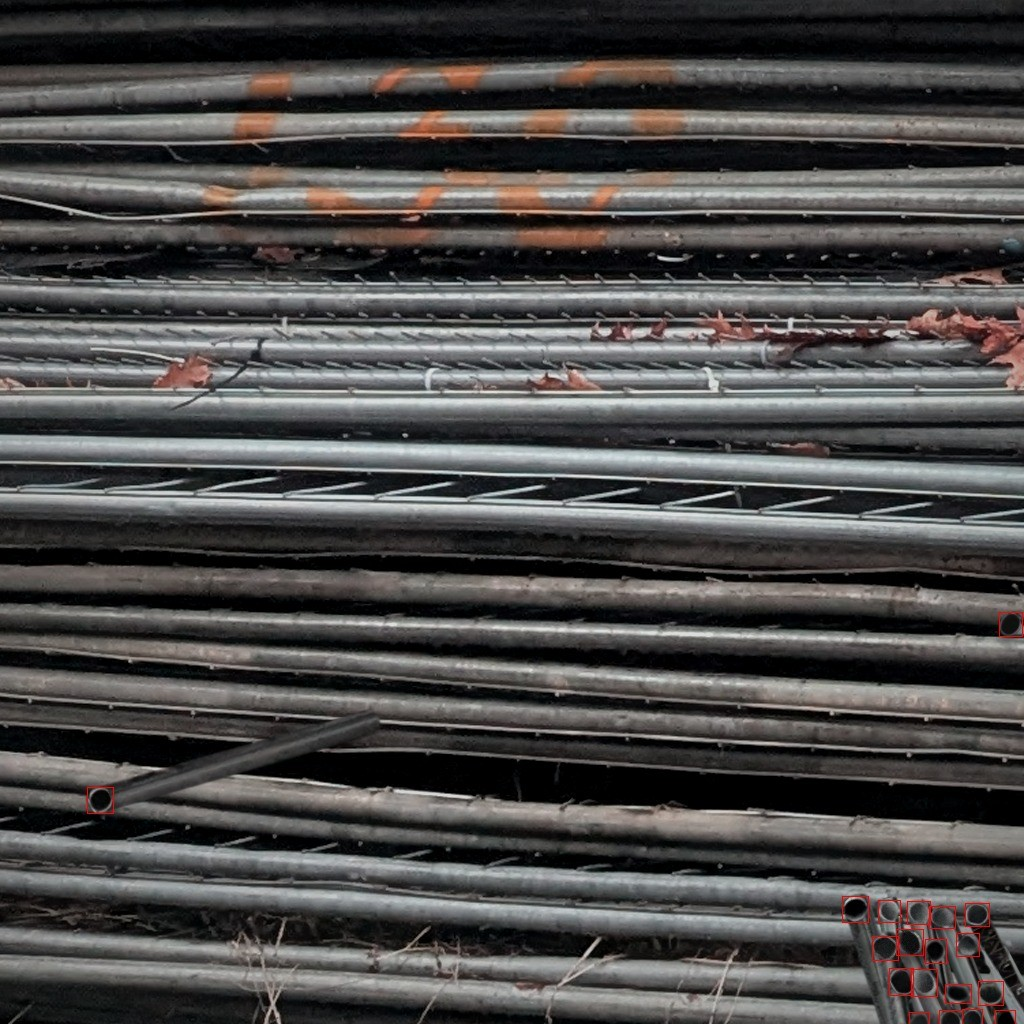
\includegraphics[width=\textwidth]{abbildungen/synth_000.jpg}
\end{subfigure}\hfill
\begin{subfigure}{0.32\textwidth}
  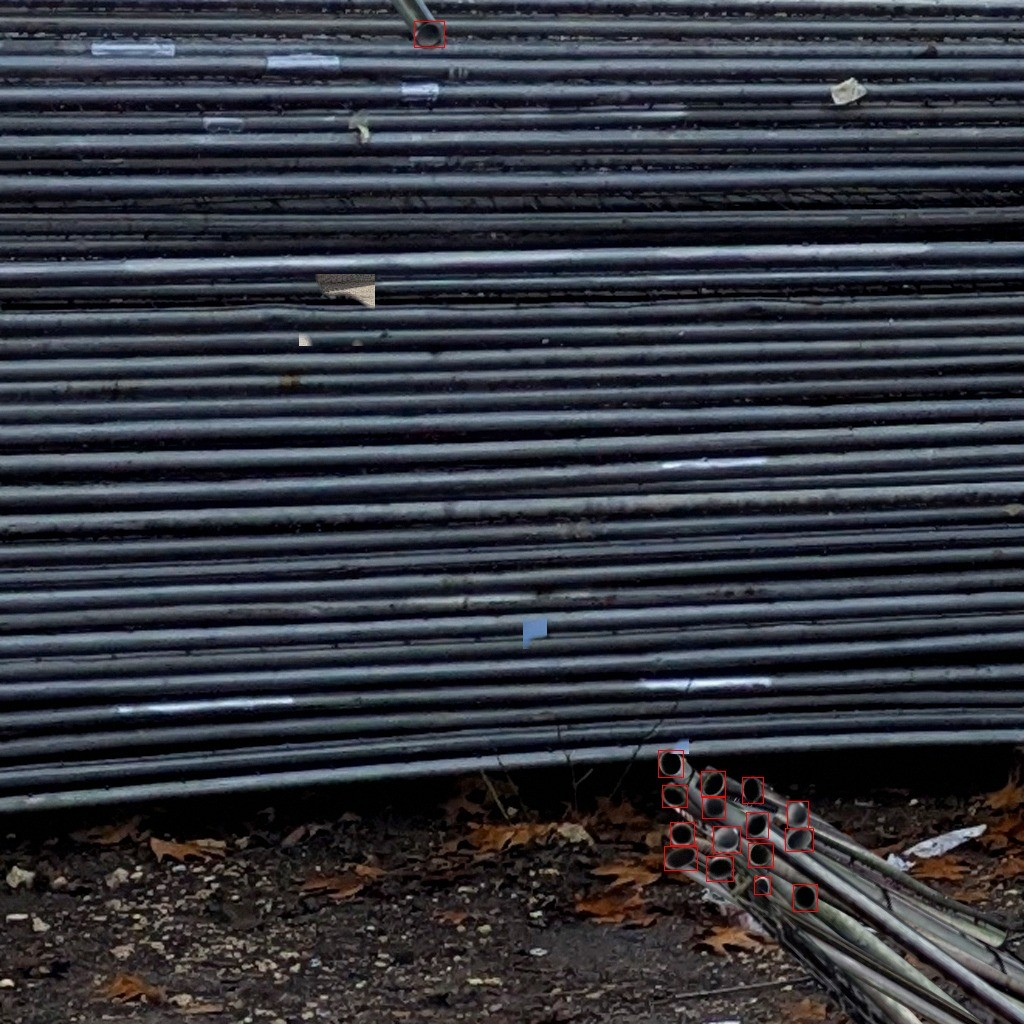
\includegraphics[width=\textwidth]{abbildungen/synth_001.jpg}
\end{subfigure}\hfill
\begin{subfigure}{0.32\textwidth}
  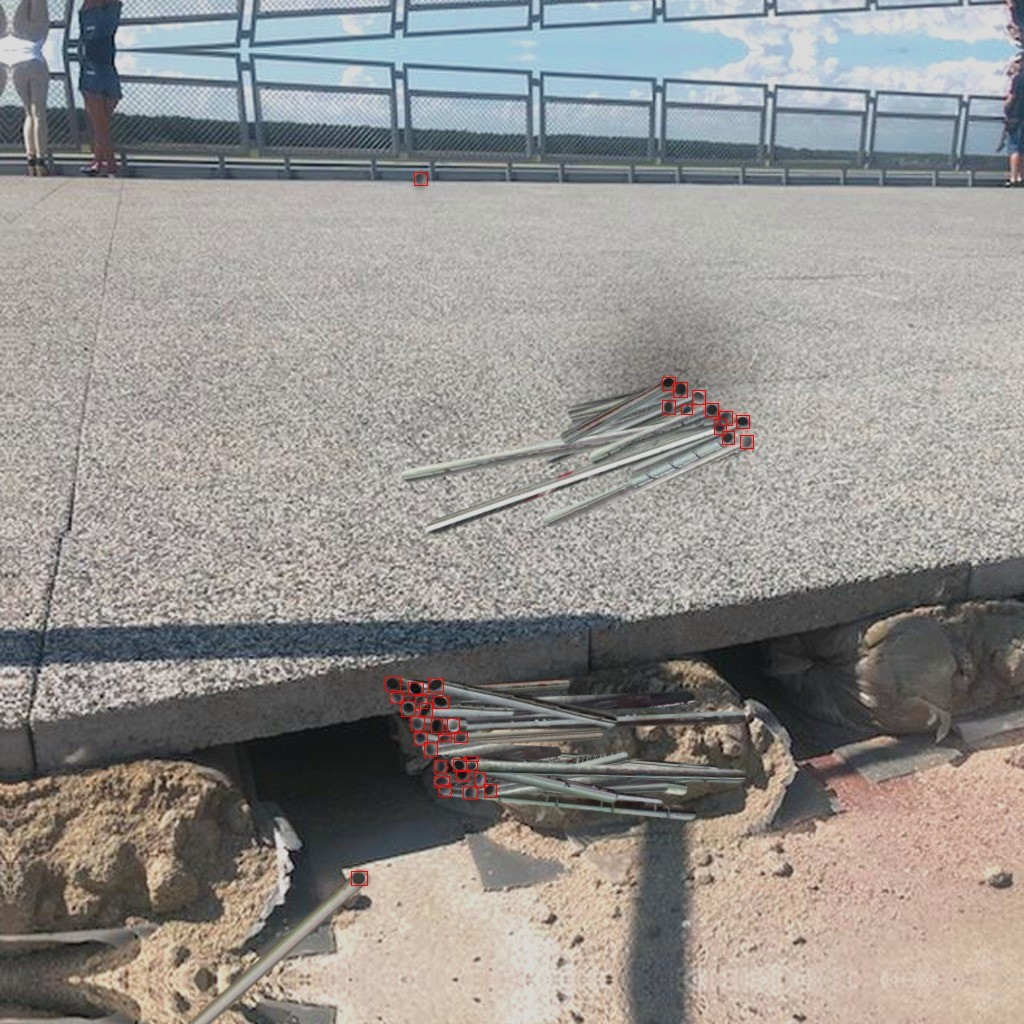
\includegraphics[width=\textwidth]{abbildungen/synth_002.jpg}
\end{subfigure}

\vspace{2mm}
\begin{subfigure}{0.32\textwidth}
  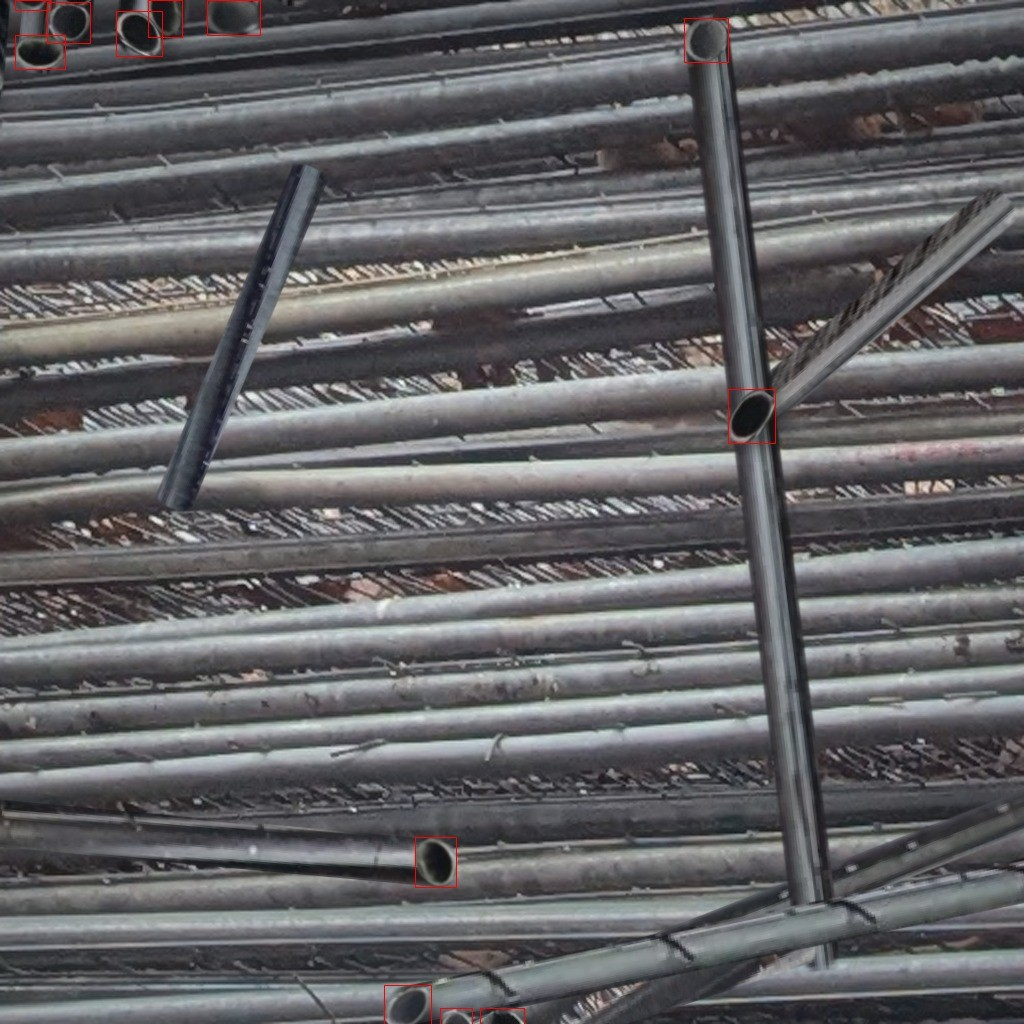
\includegraphics[width=\textwidth]{abbildungen/synth_003.jpg}
\end{subfigure}\hfill
\begin{subfigure}{0.32\textwidth}
  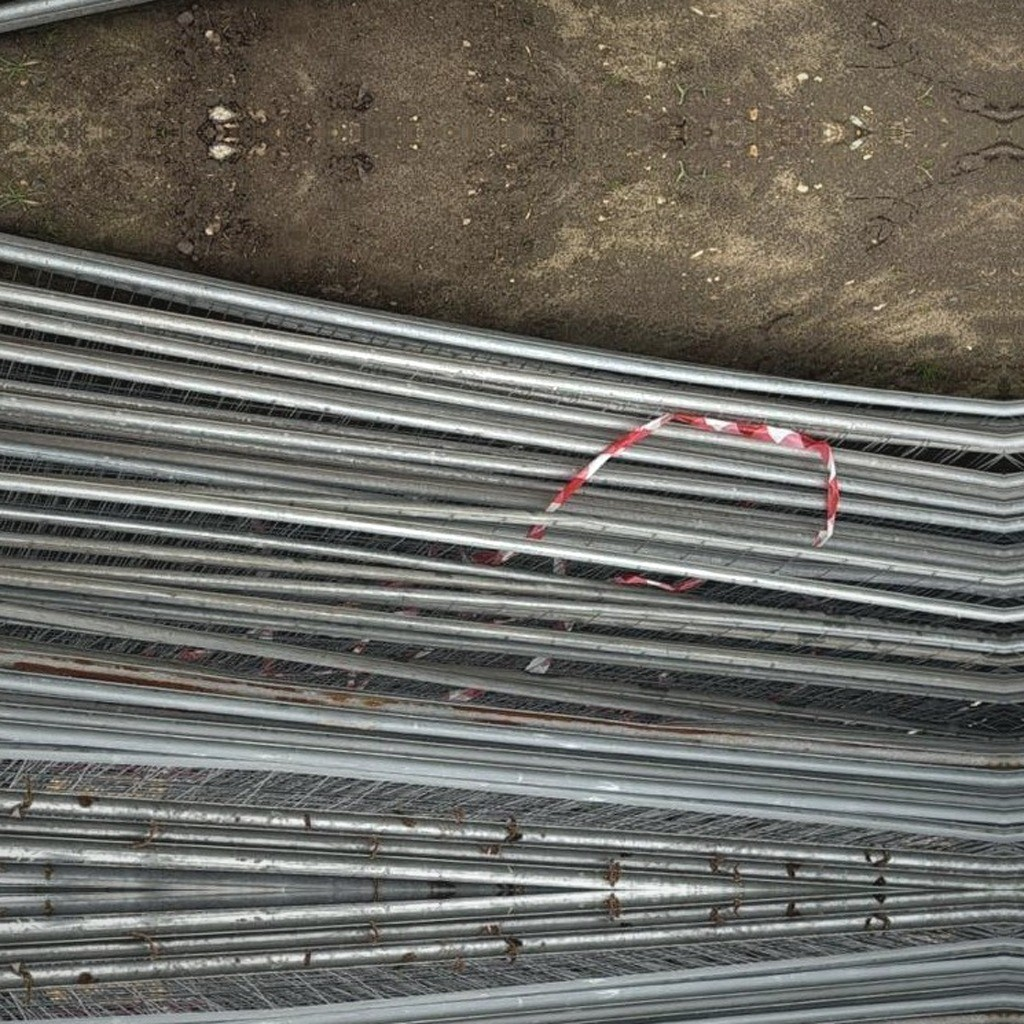
\includegraphics[width=\textwidth]{abbildungen/synth_004.jpg}
\end{subfigure}\hfill
\begin{subfigure}{0.32\textwidth}
  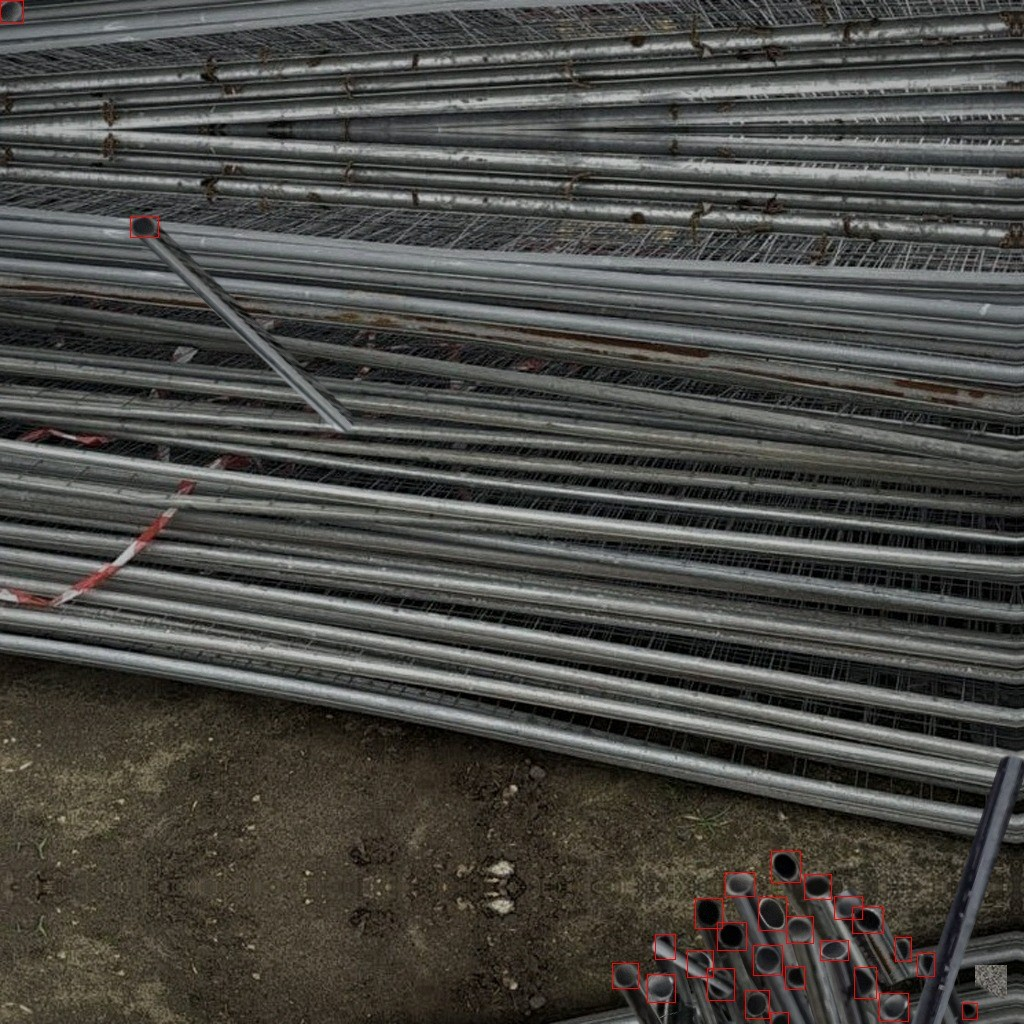
\includegraphics[width=\textwidth]{abbildungen/synth_005.jpg}
\end{subfigure}
\caption[Beispiele synthetischer Trainingsbilder]{Sechs synthetische
Trainingsbilder mit eingezeichneten erzeugten Labels. Erkennbar sind die
Clusterstruktur des Layoutmodells, die Rohrschäfte hinter den Stirnflächen, die
quer liegenden Okkluder und die abgedunkelten Mulden. Am unteren Rand des
mittleren Bildes der unteren Reihe ist die in
Abschnitt~\ref{sec:grenzen} genannte Spiegelsymmetrie des Reflect-Paddings
sichtbar.}
\label{abb:synthbeispiele}
\end{figure}

\section{Nachweis der Anforderungen}
\label{sec:nachweis}

Tabelle~\ref{tab:nachweis} prüft die in Abschnitt~\ref{sec:anforderungen}
aufgestellten Anforderungen gegen die umgesetzte Pipeline.

\begin{table}[htbp]
\centering
\caption[Nachweis der Anforderungen A1--A6]{Nachweis der Anforderungen aus
Abschnitt~\ref{sec:anforderungen}.}
\label{tab:nachweis}
\footnotesize
\begin{tabularx}{\textwidth}{@{}L{0.07\textwidth}XL{0.12\textwidth}@{}}
\toprule
\textbf{Anf.} & \textbf{Umsetzung} & \textbf{Status} \\
\midrule
A1 & Box wird nach jeder Instanztransformation aus der transformierten
Alphamaske neu bestimmt; \code{degrees}, \code{shear}, \code{perspective} zur
Trainingszeit auf 0 & erfüllt \\
A2 & Objektgrößen 12--44\px{} aus der Realmessung; Leinwand
$1024 = $ \code{imgsz}, also keine Skalierung im Training & erfüllt \\
A3 & Zoom an Rohrdurchmesser gekoppelt; Schaft hinter jeder Stirnfläche;
parallele Schaftrichtung; Tiefenmodell 75/25; Rotation voll, weil physikalisch
unbeschränkt & erfüllt \\
A4 & S1 Alphamaske + Kantenweichzeichnung; S2 partieller Farbangleich; S3
flächentreue Skalierung + Unschärfeangleich; S4 lokal geschätzter Rauschangleich;
S5 JPEG-Requantisierung; S6 Schlagschatten + physikalische Verdeckung & erfüllt \\
A5 & modale Boxen; Verwerfen unter 30\,\% Sichtbarkeit bzw.\ 15\,\%
Bildanteil -- dieselben Regeln wie bei der Handannotation & nur annähernd
erfüllt: Restversatz der Boxgröße 1,2--2,5\px{}
(Abschnitt~\ref{sec:boxversatz}) \\
A6 & 36 Transformationen mit Soll-Bereich und gemessenem Ist-Anteil
(Tabellen~\ref{tab:t1}--\ref{tab:t8}); sechs Werte ausdrücklich als Annahme
gekennzeichnet & erfüllt \\
\bottomrule
\end{tabularx}
\end{table}

Die Anforderungen sind damit formal erfüllt. Das sagt allerdings nichts darüber
aus, ob die einzelnen Maßnahmen \emph{wirken} -- Erfüllung einer
Entwurfsanforderung ist kein empirischer Nachweis. Diese Unterscheidung wird in
Kapitel~\ref{kap:auswertung} durch die Messung des Sim-to-Real-Abstands und die
Okklusionsablation adressiert und in Abschnitt~\ref{sec:tragend} explizit
bilanziert.

\chapter{Training und Trainingszeit-Augmentierung}
\label{kap:trainingszeit}

\section{Aufbau}
\label{sec:trainingsaufbau}

\absatz{Datenaufteilung.} Trainiert wird auf synthetischen Bildern,
validiert auf dem \emph{realen} \code{val}-Bild (98 Objekte). Das ist eine
bewusste Entscheidung: Die Modellauswahl muss auf der Zieldomäne erfolgen, sonst
wählt man das Modell, das am besten zu den eigenen Renderartefakten passt.
\code{test} (89 Objekte) berührt Training und Modellauswahl nie und dient
ausschließlich der Endbewertung. Ein vierter Split \code{sval} aus 400
synthetischen Bildern mit anderem Seed dient allein der Messung des
Sim-to-Real-Abstands (Abschnitt~\ref{sec:simtoreal}).

\absatz{Zwei Budgets.} Die Arbeit trainiert Modelle in zwei Größenordnungen, und
es ist wichtig, sie nicht zu vermischen (Tabelle~\ref{tab:budgets}). Das
\textbf{Referenzmodell} nutzt den vollen Datensatz aus 6000 Bildern und
60~Epochen; es ist das Modell, dessen Zahlen als Ergebnis der Pipeline berichtet
werden (Abschnitt~\ref{sec:hauptergebnis}). Die \textbf{Ablationsarme} nutzen
jeweils 3000~Bilder und 30~Epochen. Dieses kleinere Budget ist eine Konzession an
die Rechenzeit -- mehrere Läufe statt einem --, und es ist \emph{für alle Arme
identisch}. Es begrenzt damit die absolute Höhe der Ablationszahlen, nicht ihren
Vergleich untereinander; Ablationszahlen sind deshalb ausschließlich mit
Ablationszahlen zu vergleichen, nie mit denen des Referenzmodells.

\begin{table}[htbp]
\centering
\caption[Die beiden Trainingsbudgets]{Die beiden Trainingsbudgets. Alles, was
nicht genannt ist, ist identisch: Architektur, Optimierer, Lernratenplan,
Verlustgewichte, Trainingszeit-Augmentierung, Seed, Validierungssplit.}
\label{tab:budgets}
\footnotesize
\begin{tabular}{@{}lcc@{}}
\toprule
 & \textbf{Referenzmodell} & \textbf{Ablationsarme (3$\times$)} \\
\midrule
Trainingsbilder & 6000 & 3000 \\
Epochenbudget & 60 (\code{patience}~20) & 30 (\code{patience}~20) \\
tatsächlich gelaufen & \zrefEpochen{} (bestes Modell: \zrefBestEpoche) & 30 \\
Batch & 8 & 8 \\
Bildzwischenspeicher & Festplatte & Festplatte \\
\bottomrule
\end{tabular}
\end{table}

Der Referenzlauf endete durch Early Stopping nach \zrefEpochen{} von
60~Epochen; das beste Modell stammt aus Epoche~\zrefBestEpoche. Die beiden
letzten Zeilen der Tabelle sind nicht gewählt, sondern erzwungen: \code{yolo26s-p2}
hält bei \code{imgsz}=1024 eine P2-Merkmalskarte mit $256\times256$ Zellen vor und
belegt bei Batch~16 rund 23,5\,GB -- alle Speicherangaben dieses Absatzes sind
mit \code{nvidia-smi} an den eigenen Läufen gemessen. Auf der verwendeten Karte waren zur Laufzeit
der Ablationen nur etwa 25\,GB frei; ein erster Lauf mit Batch~16 wich wiederholt
mit \code{CUDA OutOfMemoryError in TaskAlignedAssigner} auf die CPU aus -- was
nicht nur langsam ist, sondern die Läufe untereinander unvergleichbar macht, weil
der Ausweichpfad von der momentanen Fremdlast abhängt. Batch~8 belegt rund
13\,GB und läuft durchgängig auf der GPU.

\absatz{Modellwahl.} Durchgängig verwendet wird \code{yolo26s-p2} mit
9,66~Millionen Parametern (Modellzusammenfassung der Werkzeugkette,
Abschnitt~\ref{sec:p2kopf}). Die \emph{Größe} \enquote{s} folgt aus der Datenlage:
Der Datensatz hat eine Klasse und nur neun zugrunde liegende Objektinstanzen, die
Formvielfalt ist klein, die nötige Modellkapazität damit ebenfalls; die
\enquote{nano}-Variante verliert bei 12--40\px{} großen Objekten Rückruf, größere
Varianten würden die synthetischen Eigenheiten eher memorieren. Der \emph{P2-Kopf}
folgt aus der Auflösungsrechnung in Abschnitt~\ref{sec:p2kopf}: Er senkt die
Schrittweite der feinsten Detektionsebene von 8 auf 4 und die Zuweisungsgrenze
damit von 11,3 auf 5,7\px{} -- unter alle in \code{val} und \code{test}
auftretenden Objektgrößen. Er kostet dabei \emph{keine} Parameter (er hat 2,9\,\%
weniger als das Basismodell), sondern Speicher.

Ausgangspunkt sind COCO-vortrainierte Gewichte: Die vortrainierten
Low-Level-Filter sind domänenunabhängig \parencite{yosinski2014}, und
\textcite{hinterstoisser2018} zeigen den Nutzen explizit für synthetische
Trainingsdaten. Weil die \code{-p2}-Variante über eine Architekturdatei und nicht
über einen fertigen Checkpoint definiert ist, werden die Gewichte
\emph{partiell} übernommen: Backbone und die Ebenen P3--P5 aus \code{yolo26s.pt},
die zusätzlichen Blöcke der P2-Ebene zufällig initialisiert.

\absatz{Modellauswahl.} Gespeichert wird der Checkpoint mit der höchsten
Fitness auf dem realen \code{val}-Bild, wobei die Fitness der Werkzeugkette
$0{,}1 \cdot \mAPfifty + 0{,}9 \cdot \mAPall$ ist -- diese Gewichtung ist deren
Voreinstellung und wurde nicht verändert. Ein Detail ist dabei
festzuhalten: Diese Validierung läuft bei der \emph{Trainings}auflösung
\code{imgsz}=1024, während alle berichteten Zahlen bei nativem Maßstab (2464
bzw.\ 1600) gemessen werden. Auswahl- und Bewertungsauflösung fallen also
auseinander. Das ist hinnehmbar, weil die Rangfolge der Epochen von der
Auflösung kaum abhängt und die Alternative -- Auswahl bei nativem Maßstab --
eine zweite Validierung je Epoche kosten würde; es ist aber eine Annahme und
keine Messung, und sie gilt für alle Läufe gleich.

\absatz{Eingabegröße.} \code{imgsz}=1024, identisch zur Leinwandgröße des
Generators. Damit durchlaufen die synthetischen Bilder \emph{keine} Skalierung,
und die Objekte erreichen das Netz mit exakt der Pixelgröße, für die die Pipeline
ausgelegt ist (Anforderung~A2). Bei 640\px{} wären sie nach Gleichung~\eqref{eq:deff} nur noch 7--27\px{} groß
und lägen teils unter der Auflösung der P3-Ebene.

\absatz{Optimierung.} AdamW \parencite{loshchilov2019} mit
$\text{lr}_0 = 10^{-3}$, Endlernrate 1\,\% davon, Kosinusabfall
\parencite{loshchilov2017sgdr}, drei Aufwärmepochen, Weight Decay $5\cdot10^{-4}$,
Mixed Precision \parencite{micikevicius2018}, fester Seed und
deterministische Kernel. AdamW ist explizit gesetzt statt \code{auto}, weil es
bei kleinen Datensätzen schneller konvergiert und robust gegenüber der
Lernratenwahl ist -- wichtig, weil kein Budget für eine Lernratensuche vorhanden
ist. Die Verlustgewichte bleiben auf den Standardwerten
(\code{box}\,7,5 / \code{cls}\,0,5): Eine Erhöhung des Boxgewichts wäre bei
kleinen Objekten denkbar, ohne separaten Abstimmungssplit aber nicht belegbar.
Die Budgets stehen in Tabelle~\ref{tab:budgets}; Early Stopping greift jeweils
nach 20 Epochen ohne Verbesserung auf dem realen \code{val}-Bild. Bewusst
großzügig: Die Fitness schwankt auf knapp hundert Ground-Truth-Objekten stark,
ein knappes Fenster bräche zu früh ab.

\section{Augmentierungsparameter zur Trainingszeit}
\label{sec:trainparam}

Die abgeschalteten Parameter sind genauso begründungspflichtig wie die aktiven --
ein auf Null gesetzter Standardwert ist eine Entscheidung.

Aktiv sind Mosaic (immer, in den letzten zehn Epochen abgeschaltet), Skalierung
$0{,}6$--$1{,}4$, Translation, horizontale und vertikale Spiegelung sowie
HSV-Variation (Ton 0,015, Sättigung 0,7, Helligkeit 0,4). Abgeschaltet sind
\code{degrees}, \code{shear} und \code{perspective}, weil Bildrotation
achsparallele Boxen aufbläht -- bei $10^\circ$ um 15,8\,\% der Kantenlänge, was
die Überlappung mit der korrekten Box auf 0,745 senkt
(Abschnitt~\ref{sec:boxrotation}) --, sowie \code{mixup} und \code{cutmix}, die
Bildinhalte bei erhaltenen Labels überlagern und damit Geisterobjekte mit vollem
Boxlabel erzeugen \parencite{zhang2018mixup,yun2019cutmix}: Bei dicht gepackten
20\px-Objekten überwiegt der Labelkonflikt. \code{erasing} entfällt, weil es in
der Werkzeugkette nur bei der Klassifikation wirkt, und \code{copy\_paste},
weil es Segmentierungsmasken benötigt -- beides übernimmt der Generator
physikalisch korrekt. Die vollständige Tabelle mit Begründung je Parameter steht
im Anhang (Tabelle~\ref{tab:trainaug}).

Die beiden Augmentierungsschichten wirken bei der Objektgröße multiplikativ: Der
Generator erzeugt $[12, 44]$\px, die Trainingsskalierung multipliziert mit
$[0{,}6;\,1{,}4]$, sodass das Netz effektiv Objekte von
$12 \cdot 0{,}6 = 7{,}2$ bis $44 \cdot 1{,}4 = 61{,}6$\px{} sieht. Diese Spanne
deckt nach unten die Objektgrößen bei niedriger Inferenzauflösung und nach oben
jene bei starker Hochskalierung ab -- also den gesamten in
Abschnitt~\ref{sec:imgsz} durchmusterten Bereich. Sie deckt zugleich die vier
Objekte unter 12\px{} ab, die \code{test} enthält und die der Generator selbst
nicht erzeugt (Abschnitt~\ref{sec:valtest}). Der untere Rand von 7,2\px{} liegt
oberhalb der Zuweisungsgrenze $S\sqrt{2} = 5{,}7$\px{} der P2-Ebene, aber
\emph{unterhalb} der Grenze 11,3\px, die ohne P2-Kopf gälte: Erst die Modellwahl
aus Abschnitt~\ref{sec:p2kopf} macht \code{scale}$\,=0{,}4$ zu einem Wert, bei
dem auch der untere Rand der Trainingsverteilung noch zuverlässig zugewiesen
wird.

\section{Trainingsverlauf}
\label{sec:trainingsverlauf}

Abbildung~\ref{abb:training} zeigt die Lernkurven der drei Ablationsarme.
Drei Beobachtungen sind unabhängig vom Ausgang der Ablation.

\emph{Erstens} fällt der Trainingsverlust über alle 30 Epochen monoton, während
die Metrik auf dem realen \code{val}-Bild deutlich früher flach wird. Das ist der
Sim-to-Real-Abstand in zeitlicher Form: Ab dem Knick verbessert das Modell
überwiegend seine Anpassung an Eigenschaften der synthetischen Daten, die in der
Zieldomäne nicht gelten. Genau deshalb ist es methodisch notwendig, das beste
Modell über den \emph{realen} Validierungssplit auszuwählen; eine synthetische
Validierung wählte das Modell aus der letzten Epoche und damit das am stärksten
überangepasste.

\emph{Zweitens} liegt der Trainingsverlust des Arms mit dem naiven Verdecker
(B2) unter dem der beiden anderen, obwohl alle drei exakt dieselben Objekte an
denselben Stellen enthalten. Das ist für sich genommen kein Qualitätsurteil --
ein niedriger Trainingsverlust auf synthetischen Daten sagt nichts über die
Zieldomäne --, aber es zeigt, dass der Eingriff gewirkt hat: Ein flächig grauer
Verdecker macht dieselbe Szene messbar leichter.

\emph{Drittens} liegt die Kurve auf dem realen Bild deutlich unruhiger als der
Trainingsverlust. Das ist kein Trainingsproblem, sondern eine Folge der
Datenlage: Die Fitness wird an 98 Objekten \emph{eines} Bildes gemessen, und ein
einzelnes gefundenes oder verlorenes Objekt verschiebt den Rückruf bereits um
einen Prozentpunkt. Aus demselben Grund ist \code{patience} mit 20 Epochen
großzügig gesetzt -- ein knappes Fenster bräche bei dieser Streuung ab, bevor
das Modell auskonvergiert ist.

\begin{figure}[htbp]
\centering
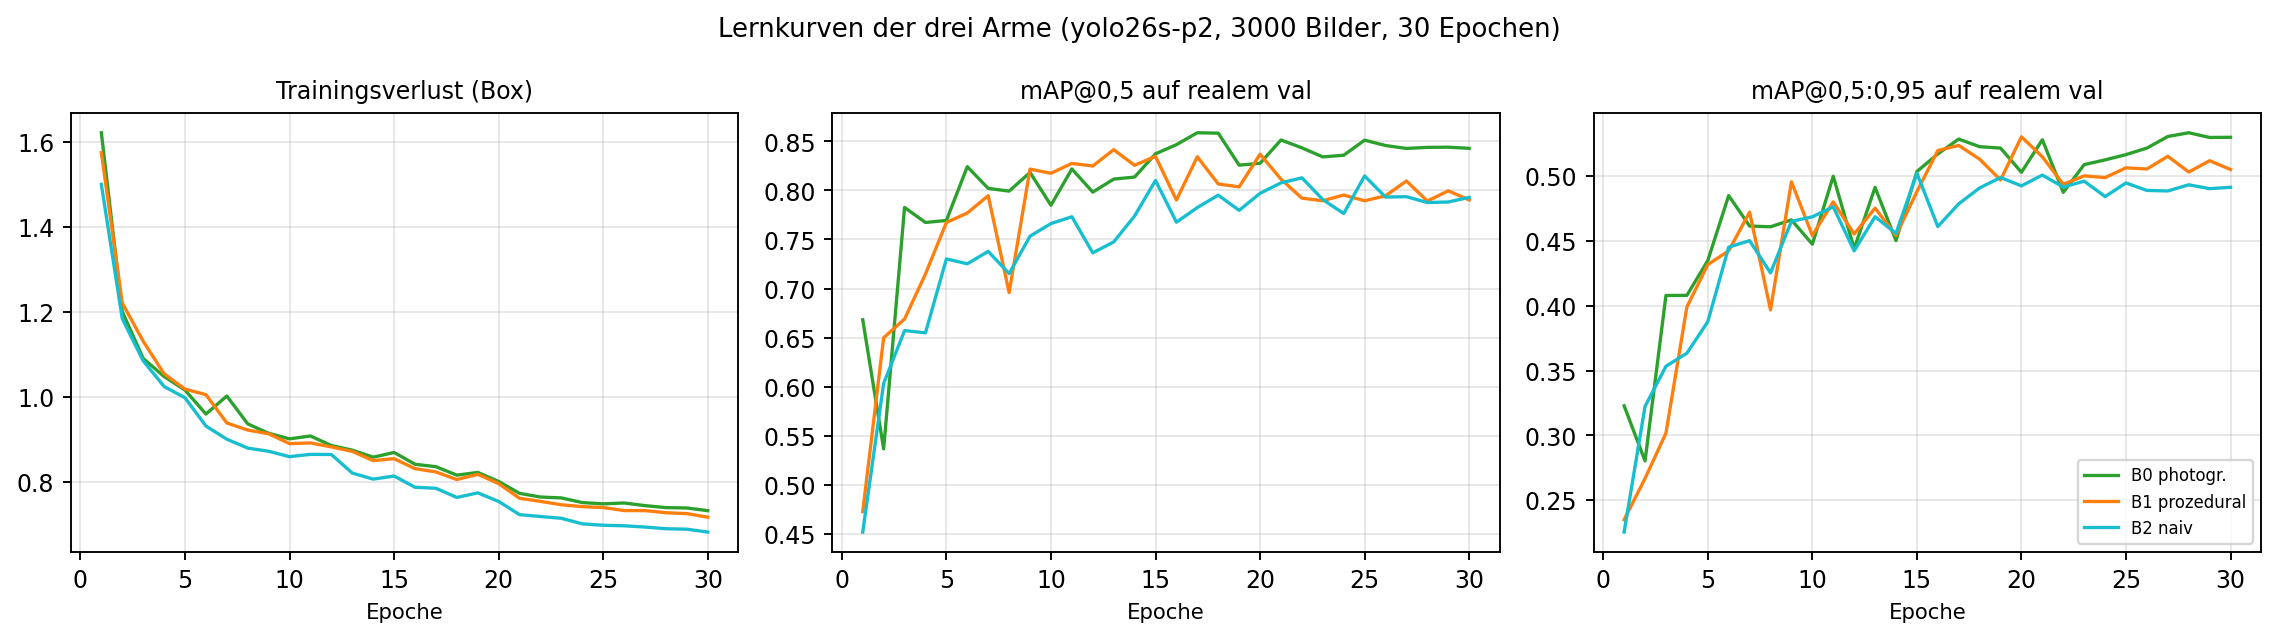
\includegraphics[width=\textwidth]{abbildungen/neu_training_b.png}
\caption[Lernkurven der Ablationsarme]{Lernkurven der drei Ablationsarme
(\code{yolo26s-p2}, 3000 Bilder, 30 Epochen, Batch~8). Links der
Box-Trainingsverlust auf den synthetischen Daten, Mitte und rechts \mAPfifty{}
und \mAPall{} auf dem realen \code{val}-Bild nach jeder Epoche. Diese
Validierung läuft bei der Trainingsauflösung \code{imgsz}=1024 und liegt
deshalb systematisch unter den in Kapitel~\ref{kap:auswertung} berichteten
Werten, die bei nativem Maßstab gemessen sind; für den \emph{Verlauf} ist das
ohne Belang. Der Knick
zwischen fallendem Verlust und flacher Realmetrik markiert den Punkt, ab dem
weiteres Training überwiegend synthetische Eigenheiten anpasst.}
\label{abb:training}
\end{figure}

\chapter{Auswertung}
\label{kap:auswertung}

Dieses Kapitel beantwortet drei Fragen: Was leistet die Pipeline auf echten Daten
(Abschnitte~\ref{sec:metriken}--\ref{sec:simtoreal})? Welche Parameter dominieren
das Ergebnis (Abschnitte~\ref{sec:imgsz} und \ref{sec:infparam})? Und trägt die
aufwendigste Augmentierungsentscheidung -- die physikalisch motivierte Verdeckung
-- ihren Aufwand (Abschnitt~\ref{sec:ablation})?

\section{Bewertungsprotokoll und Metriken}
\label{sec:metriken}

\subsection{Die verwendeten Metriken in Worten}

Damit die folgenden Zahlen lesbar sind, seien die Metriken zunächst knapp und
anschaulich erklärt. Eine Detektion gilt als Treffer (\emph{True Positive}, TP),
wenn ihre Box eine Ground-Truth-Box mit einer Überlappung von mindestens $t$
umschließt; die Überlappung wird als \emph{Intersection over Union} gemessen:
\begin{equation}
\mathrm{IoU}(A, B) = \frac{|A \cap B|}{|A \cup B|}.
\end{equation}
Jede Ground-Truth-Box kann höchstens einmal getroffen werden; überzählige
Detektionen sind Falsch-Positive (FP), nicht getroffene Ground-Truth-Boxen sind
Falsch-Negative (FN). Daraus folgen:

\begin{description}[leftmargin=4.6em,style=sameline,font=\normalfont\itshape]
  \item[Precision] $P = \mathrm{TP}/(\mathrm{TP}+\mathrm{FP})$ -- der Anteil der
  Detektionen, die richtig sind. Wenig FP bedeutet hohe Precision.
  \item[Recall] $R = \mathrm{TP}/(\mathrm{TP}+\mathrm{FN})$ -- der Anteil der
  vorhandenen Objekte, die gefunden wurden.
  \item[F1] das harmonische Mittel $2PR/(P+R)$. Berichtet wird das \emph{beste}
  F1 über alle Konfidenzschwellen sowie die zugehörige Schwelle $c^*$; das ist
  der Betriebspunkt, den man in einer Anwendung wählen würde.
  \item[AP / mAP] die Fläche unter der Precision-Recall-Kurve
  \parencite{everingham2010}. \mAPfifty{} verwendet $t = 0{,}5$, \mAPseven{}
  $t=0{,}75$, \mAPall{} den Mittelwert über $t = 0{,}50; 0{,}55; \dots; 0{,}95$
  nach COCO-Konvention \parencite{lin2014coco}. Da hier nur eine Klasse existiert,
  ist mAP mit AP identisch.
  \item[Zählfehler] die für die Anwendung eigentlich relevante Größe: die
  Differenz zwischen der Anzahl der Detektionen am Betriebspunkt $c^*$ und der
  Anzahl der Ground-Truth-Objekte.
\end{description}

Zwei Lesehinweise sind wichtig. Erstens sagt ein hoher \mAPfifty{}-Wert bei
gleichzeitig niedrigem \mAPseven{}-Wert, dass die Objekte \emph{gefunden}, aber
nicht präzise \emph{lokalisiert} werden -- bei 20\px{} großen Objekten ist das
nach Gleichung~\eqref{eq:ioushift} zu erwarten. Zweitens ist der Zählfehler nicht
aus mAP ableitbar: Er hängt zusätzlich davon ab, ob sich FP und FN gegenseitig
kompensieren.

\subsection{Eigenes Bewertungsframework und seine Verifikation}

Die Bewertung erfolgt über eine eigene Implementierung
(\code{src/evaluate.py}) und nicht über die Bewertungsfunktion der
Werkzeugkette. Der Grund ist, dass Zählfehler, mittlere Treffer-IoU und der
F1-optimale Betriebspunkt gebraucht werden -- Größen, die die Standardfunktion
nicht ausgibt -- und dass die Zuordnungslogik nachvollziehbar sein muss.

Eine eigene Metrikimplementierung ist allerdings eine Fehlerquelle. Sie wird
deshalb gegen die Referenzimplementierung geprüft
(Tabelle~\ref{tab:crosscheck}).

\begin{table}[htbp]
\centering
\caption[Verifikation der Metrikimplementierung]{Verifikation der eigenen
Metrikimplementierung gegen die Referenzimplementierung der Werkzeugkette,
nativer Maßstab.}
\label{tab:crosscheck}
\small
\begin{tabular}{@{}lcc@{}}
\toprule
 & \textbf{eigene Implementierung} & \textbf{Referenz} \\
\midrule
\code{val} \mAPfifty{} / \mAPall{}  & 0{,}886 / 0{,}597 & 0{,}897 / 0{,}599 \\
\code{test} \mAPfifty{} / \mAPall{} & 0{,}888 / 0{,}437 & 0{,}891 / 0{,}424 \\
\bottomrule
\end{tabular}
\end{table}

Die Abweichung liegt bei maximal 1,3\PP{} und ist durch Detailunterschiede in
der AP-Interpolation und der Zuordnungsreihenfolge erklärbar. Die eigene
Implementierung ist damit verifiziert; alle folgenden Zahlen stammen aus ihr,
sodass sie untereinander vergleichbar sind.

\section{Hauptergebnis}
\label{sec:hauptergebnis}

\begin{table}[htbp]
\centering
\caption[Hauptergebnis]{Ergebnis des besten Modells bei nativem Maßstab.
$c^*$ ist die F1-optimale Konfidenzschwelle, \enquote{mittl.\ IoU} die mittlere
Überlappung der Treffer.}
\label{tab:hauptergebnis}
\footnotesize
\resizebox{\textwidth}{!}{%
\begin{tabular}{@{}lrrrrrrrrr@{}}
\toprule
\textbf{Split} & \mAPfifty{} & \mAPseven{} & \mAPall{} & \textbf{bestes F1} &
$c^*$ & $P$ & $R$ & \textbf{mittl.\ IoU} & \textbf{Zählung} \\
\midrule
\code{val} (real)  & 0{,}886 & 0{,}793 & 0{,}597 & 0{,}862 & 0{,}336 & 0{,}872 & 0{,}852 & 0{,}824 & 86/88 \\
\code{test} (real) & 0{,}888 & 0{,}320 & 0{,}437 & 0{,}894 & 0{,}263 & 0{,}905 & 0{,}884 & 0{,}748 & 84/86 \\
\code{sval} (synth.) & 0{,}982 & 0{,}935 & 0{,}828 & 0{,}964 & 0{,}450 & 0{,}972 & 0{,}956 & 0{,}899 & 7128/7248 \\
\bottomrule
\end{tabular}}
\end{table}

\absatz{Wie ist das zu lesen?} Ein ausschließlich auf synthetischen Bildern
trainiertes Modell findet auf echten, nie im Training gesehenen Aufnahmen etwa
88--89\,\% der Objekte bei vergleichbarer Precision. Für die eigentliche
Anwendung ist der Zählfehler die relevante Größe: 86 statt 88 und 84 statt 86
Objekte, also \textbf{2,3\,\% Zählfehler} auf beiden realen Aufnahmen. Bei der
auf \code{val} gewählten Inferenzauflösung (Abschnitt~\ref{sec:imgsz}) steigt
\mAPfifty{} auf \code{test} auf 0,928, mit Test-Time-Augmentation auf 0,934.

\absatz{Der auffällige Unterschied zwischen den Splits.} \code{val} erreicht
\mAPseven{} = 0,793, \code{test} nur 0,320 -- bei praktisch identischem
\mAPfifty{}. Das ist kein Widerspruch, sondern der in
Abschnitt~\ref{sec:ioukleinobjekt} vorhergesagte Effekt: Die Objekte in
\code{test} sind kleiner (Median 19,6\px{} gegen 27,4\px{}). Nach
Gleichung~\eqref{eq:ioushift} kostet bei einem 20\px{}-Objekt ein Boxfehler von
2\px{} bereits 0,18 IoU. Die mittlere Treffer-IoU bestätigt das direkt: 0,824 auf
\code{val}, 0,748 auf \code{test}.

Die Objektgröße ist allerdings nur ein Teil der Erklärung. Den größeren Teil
liefert ein \emph{systematischer Größenversatz zwischen Generatorlabel und
Handannotation}, der in Abschnitt~\ref{sec:boxversatz} aufgeschlüsselt wird: Auf
\code{test} sind die vorhergesagten Boxen im Median 11,6\,\% kleiner als die
annotierten, auf \code{val} nur 3,9\,\%. Eine Sensitivitätsrechnung, die diesen
Versatz herausrechnet, hebt \mAPseven{} auf \code{test} von 0,320 auf 0,714.
\mAPall{} ist bei dieser Objektgröße folglich weniger ein Maß für die
Detektionsqualität als für Pixelauflösung und Labelkonvention -- eine
Feststellung, die für die Interpretation aller folgenden Tabellen gilt.

\begin{figure}[htbp]
\centering
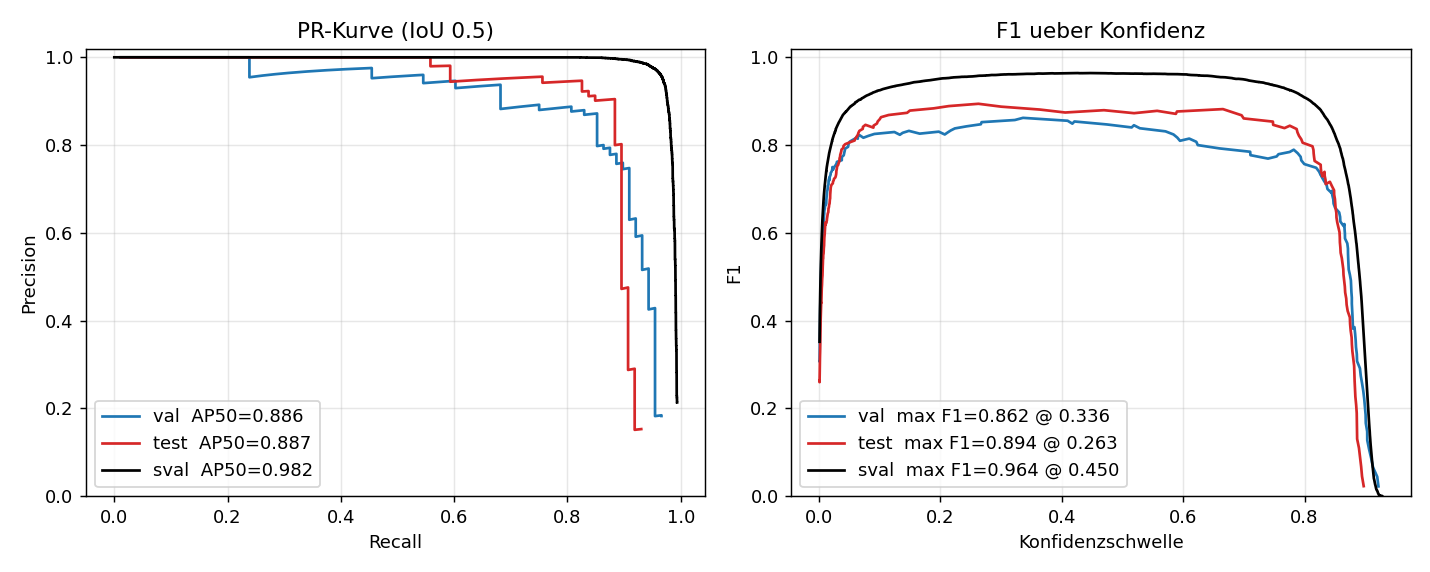
\includegraphics[width=\textwidth]{abbildungen/pr_kurven.png}
\caption[Precision-Recall-Kurven]{Precision-Recall-Kurven der drei Splits. Der
Abstand zwischen der synthetischen Kurve (\code{sval}) und den beiden realen
Kurven ist der Sim-to-Real-Abstand aus Abschnitt~\ref{sec:simtoreal}.}
\label{abb:prkurven}
\end{figure}

\begin{figure}[htbp]
\centering
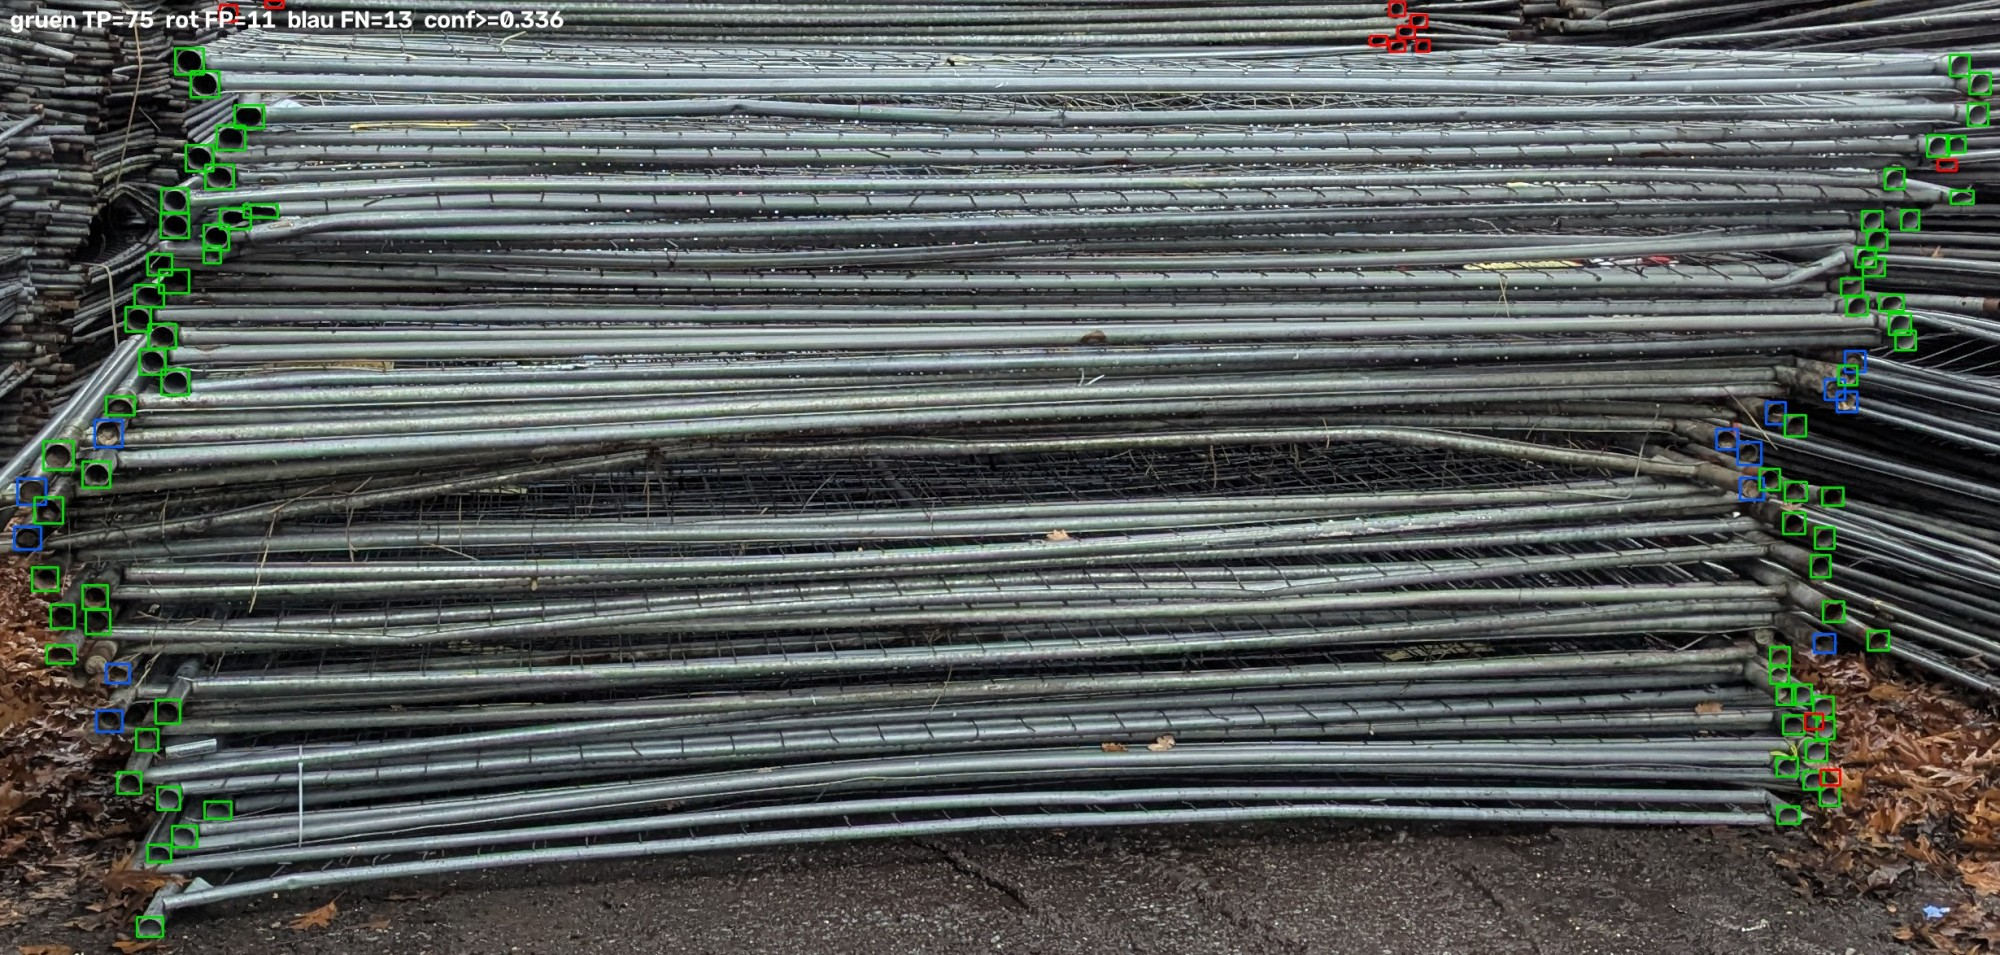
\includegraphics[width=\textwidth]{abbildungen/qual_val.jpg}

\vspace{2mm}
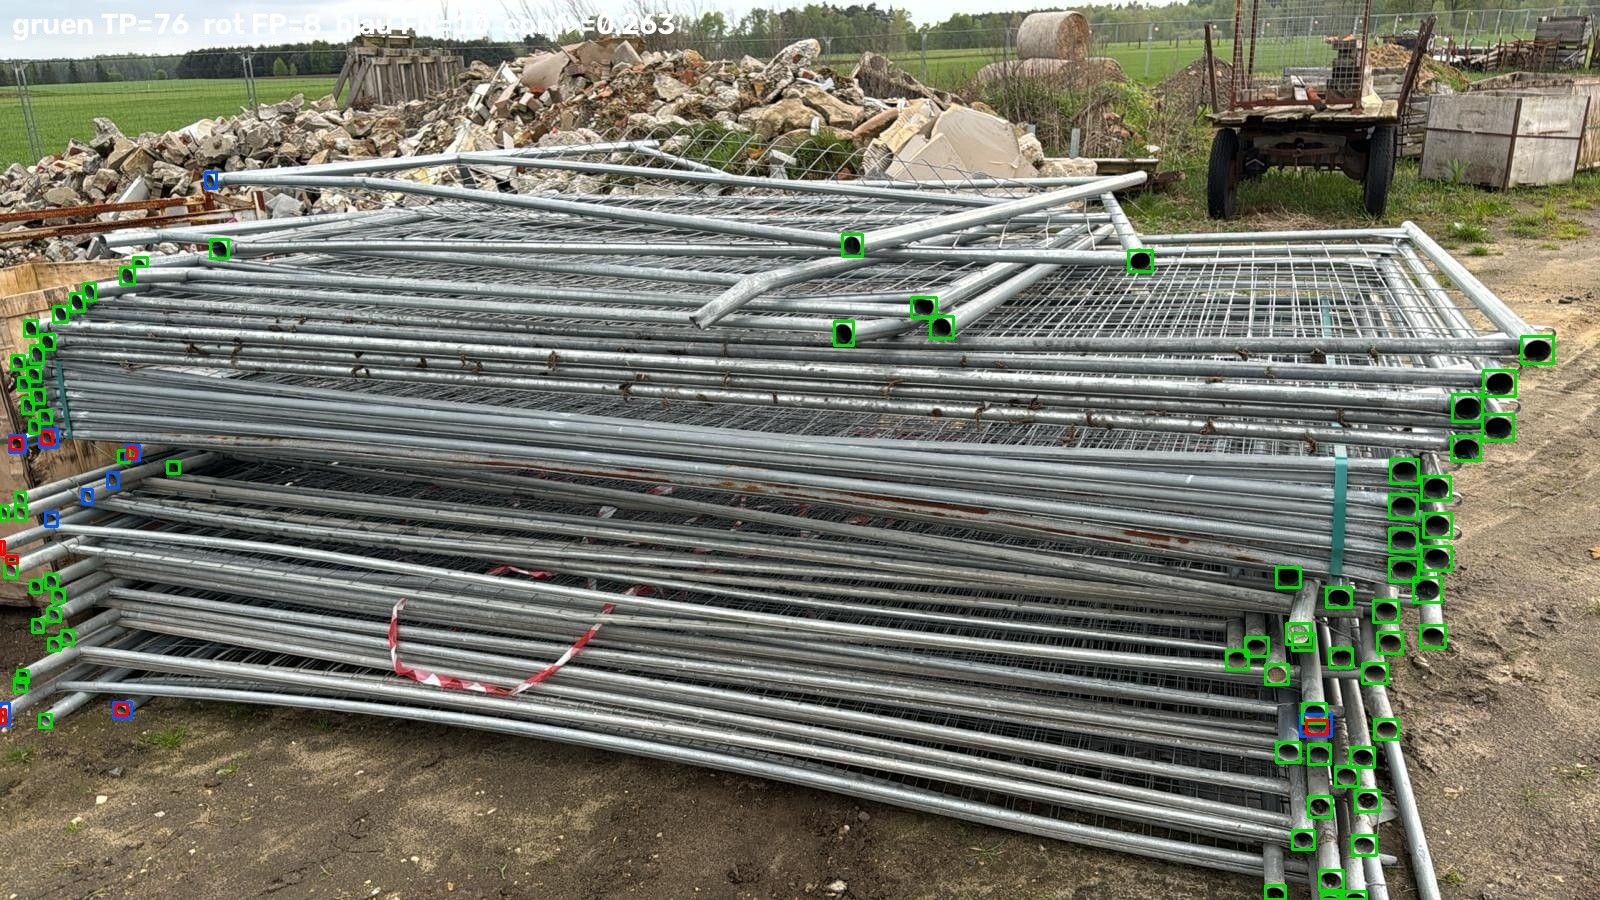
\includegraphics[width=\textwidth]{abbildungen/qual_test.jpg}
\caption[Qualitative Ergebnisse]{Qualitative Ergebnisse auf \code{val} (oben)
und \code{test} (unten). Grün = Treffer, rot = Falsch-Positiv, blau =
Falsch-Negativ. Im oberen Bild sitzen mehrere rot markierte Detektionen auf
erkennbaren Rohröffnungen, die in der Ground Truth fehlen; im unteren liegen rote
und blaue Boxen an mehreren Stellen nahezu deckungsgleich -- dasselbe Objekt zählt
dort doppelt als Fehler (Abschnitte~\ref{sec:fehleranalyse}
und~\ref{sec:boxversatz}).}
\label{abb:qualitativ}
\end{figure}

\section{Der Sim-to-Real-Abstand}
\label{sec:simtoreal}

Der Split \code{sval} besteht aus 400 synthetischen Bildern derselben Pipeline,
aber mit anderem Seed. Er ist damit die einzige Möglichkeit, die beiden
Fehlerquellen zu trennen: \emph{Kann das Modell die Aufgabe überhaupt?} und
\emph{überträgt es sich auf echte Bilder?}

\begin{equation}
\underbrace{0{,}982}_{\text{\code{sval}}}
\;-\;
\underbrace{0{,}886 \,/\, 0{,}888}_{\text{\code{val} / \code{test}}}
\;=\;
\textbf{9{,}6 bzw.\ 9{,}5 Prozentpunkte } \mAPfifty{}
\end{equation}

Bei \mAPall{} ist der Abstand mit 23,1 (\code{val}) bzw.\ 39,1 (\code{test})
Prozentpunkten deutlich größer -- was nach dem vorigen Abschnitt zu erwarten
ist, da die synthetischen Objekte im Median mit 22,5\px{} etwas größer sind als
die von \code{test}.

\absatz{Interpretation in beide Richtungen.} Der Abstand ist eine gute Nachricht
in zwei Hinsichten:

\begin{itemize}
  \item Er ist \textbf{klein genug}, dass das Verfahren praktisch funktioniert.
  Ein rein synthetisch trainiertes Modell verliert auf echten Bildern etwa
  10\PP{} -- und liegt damit noch in einem Bereich, in dem der Zählfehler unter
  3\,\% bleibt.
  \item Er ist \textbf{groß genug}, um zu belegen, dass das Netz \emph{nicht}
  bloß Einfügeartefakte gelernt hat. Wäre die Pipeline an einer der Signaturen
  S1--S6 durchlässig, so wäre \code{sval} nahezu perfekt ($>0{,}99$) und die
  realen Bilder katastrophal. Genau dieses Muster tritt nicht auf.
\end{itemize}

Dieses Argument ist der einzige \emph{direkte} empirische Hinweis darauf, dass
die Anti-Abkürzungs-Maßnahmen aus Abschnitt~\ref{sec:photometrie} und
\ref{sec:globalstufe} greifen. Es ist ein Indiz und kein Beweis: Ein
kontrollierter Nachweis müsste je Signatur einen eigenen Trainingslauf
vergleichen. Die Grenzen dieses Schlusses werden in
Abschnitt~\ref{sec:tragend} bilanziert.

\section{Experiment 1: die Inferenzauflösung}
\label{sec:imgsz}

Die Inferenzauflösung ist der einzige hier untersuchte Parameter, der nach dem
Training noch frei ist, und deshalb der einzige, dessen Wert gemessen statt
begründet wird. Gemustert werden neun Stufen zwischen 640 und 2464\px{} sowie
der native Maßstab. Ausgewählt wird die Stufe mit dem höchsten \mAPall{} auf
\code{val}, und zwar ausschließlich dort; der so gefundene Wert wird unverändert
auf beide Splits angewandt -- eine Wahl je Split wäre eine
Hyperparameterselektion auf dem Testsatz und würde dessen Zahlen wertlos machen.
Das Kriterium ist bewusst \mAPall{} und nicht \mAPfifty{}, weil es die
Lokalisierungsgüte mitbewertet; es stand vor den Läufen fest und gilt
unverändert für alle drei in Abschnitt~\ref{sec:modelle} verglichenen Modelle.
Für die Baseline fallen beide Metriken auseinander: \mAPfifty{} ist bei 1600 am
höchsten, \mAPall{} bei 1920; gewählt wurde daher 1920.

\begin{table}[htbp]
\centering
\caption[Sweep der Inferenzauflösung]{Sweep der Inferenzauflösung
\code{imgsz}. \enquote{pred} ist die Zahl der Detektionen am Betriebspunkt,
\enquote{gt} die Zahl der Ground-Truth-Objekte. Nativer Maßstab ist 2464
(\code{val}) bzw.\ 1600 (\code{test}).}
\label{tab:imgsz}
\footnotesize
\begin{tabular}{@{}lrrrrrrrr@{}}
\toprule
\textbf{Split} & \code{imgsz} & \mAPfifty{} & \mAPall{} & \textbf{bestes F1} &
$R$ & $P$ & \textbf{mittl.\ IoU} & \textbf{pred/gt} \\
\midrule
\code{val} & 640  & 0{,}435 & 0{,}201 & 0{,}507 & 0{,}398 & 0{,}700 & 0{,}711 & 50/88 \\
\code{val} & 800  & 0{,}793 & 0{,}428 & 0{,}768 & 0{,}659 & 0{,}921 & 0{,}737 & 63/88 \\
\code{val} & 960  & 0{,}852 & 0{,}498 & 0{,}840 & 0{,}773 & 0{,}919 & 0{,}773 & 74/88 \\
\code{val} & 1024 & 0{,}868 & 0{,}546 & 0{,}876 & 0{,}841 & 0{,}914 & 0{,}802 & 81/88 \\
\code{val} & 1280 & 0{,}887 & 0{,}577 & 0{,}861 & 0{,}841 & 0{,}881 & 0{,}808 & 84/88 \\
\code{val} & 1600 & \textbf{0{,}904} & 0{,}606 & 0{,}850 & 0{,}898 & 0{,}806 & 0{,}820 & 98/88 \\
\code{val} & 1920 & 0{,}893 & 0{,}613 & 0{,}851 & 0{,}909 & 0{,}800 & 0{,}830 & 100/88 \\
\code{val} & 2240 & 0{,}880 & 0{,}588 & 0{,}843 & 0{,}852 & 0{,}833 & 0{,}825 & 90/88 \\
\code{val} & 2464 & 0{,}886 & 0{,}597 & 0{,}862 & 0{,}852 & 0{,}872 & 0{,}824 & 86/88 \\
\midrule
\code{test} & 640  & 0{,}524 & 0{,}335 & 0{,}620 & 0{,}465 & 0{,}930 & 0{,}790 & 43/86 \\
\code{test} & 800  & 0{,}665 & 0{,}363 & 0{,}699 & 0{,}593 & 0{,}850 & 0{,}753 & 60/86 \\
\code{test} & 960  & 0{,}889 & 0{,}430 & 0{,}855 & 0{,}826 & 0{,}887 & 0{,}733 & 80/86 \\
\code{test} & 1024 & 0{,}882 & 0{,}459 & 0{,}841 & 0{,}767 & 0{,}930 & 0{,}740 & 71/86 \\
\code{test} & 1280 & 0{,}900 & 0{,}449 & 0{,}907 & 0{,}849 & 0{,}973 & 0{,}744 & 75/86 \\
\code{test} & 1600 & 0{,}888 & 0{,}437 & 0{,}894 & 0{,}884 & 0{,}905 & 0{,}748 & 84/86 \\
\code{test} & 1920 & \textbf{0{,}928} & 0{,}448 & 0{,}917 & 0{,}895 & 0{,}939 & 0{,}745 & 82/86 \\
\code{test} & 2240 & 0{,}928 & 0{,}457 & 0{,}920 & 0{,}872 & 0{,}974 & 0{,}744 & 77/86 \\
\code{test} & 2464 & 0{,}927 & 0{,}454 & 0{,}928 & 0{,}895 & 0{,}963 & 0{,}743 & 80/86 \\
\bottomrule
\end{tabular}
\end{table}

\begin{figure}[htbp]
\centering
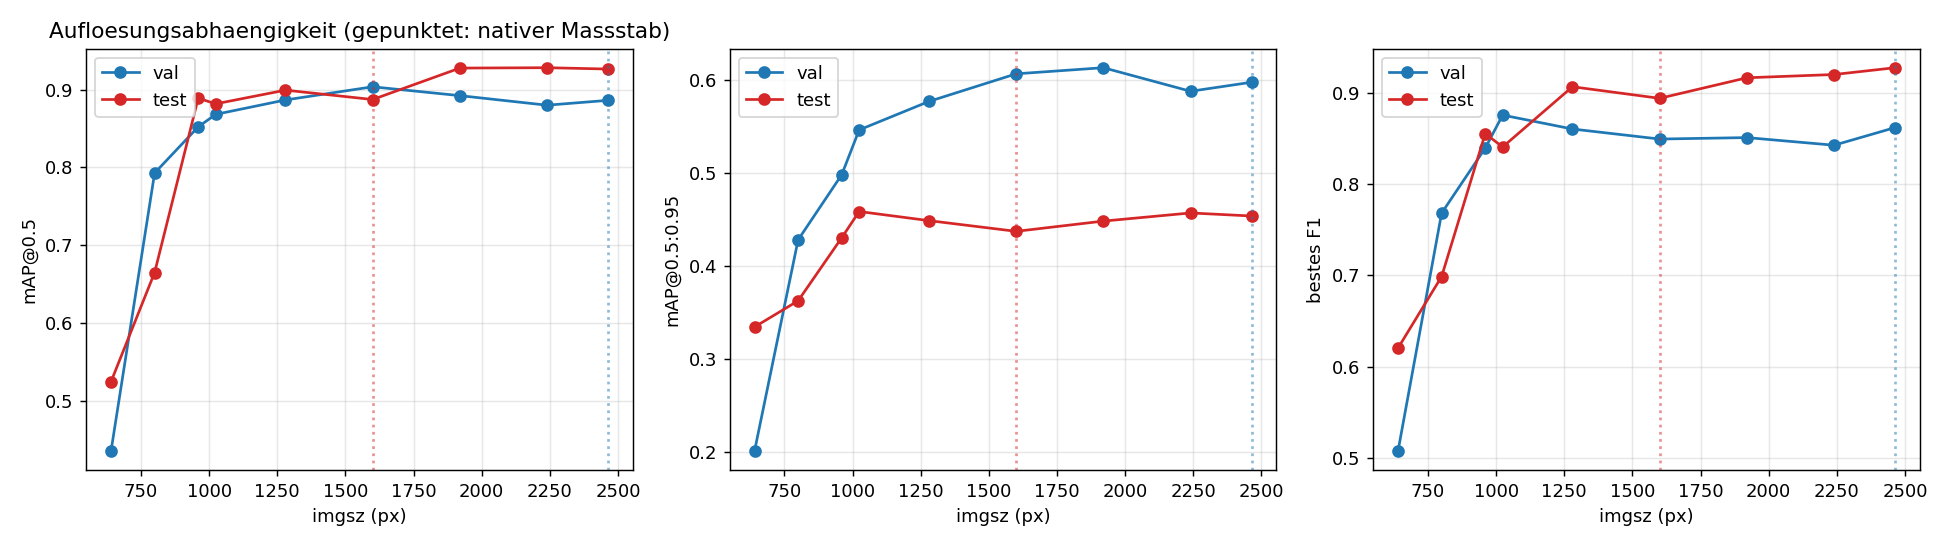
\includegraphics[width=\textwidth]{abbildungen/imgsz_sweep.png}
\caption[Sweep der Inferenzauflösung]{Sweep der Inferenzauflösung. Von 640 auf
1600\px{} verdoppelt sich \mAPfifty{} auf \code{val}; ab etwa 1280\px{} sättigt
die Kurve.}
\label{abb:imgsz}
\end{figure}

\absatz{Der größte Einzeleffekt der gesamten Arbeit.} Von \code{imgsz}~640 auf
1600 steigt \mAPfifty{} auf \code{val} von 0,435 auf 0,904 -- eine Verdopplung.
Dieser Effekt ist größer als jede einzelne Entscheidung in der
Augmentierungspipeline. Das ist ein für die Praxis unbequemes, aber wichtiges
Ergebnis: Die sorgfältigste Datensynthese wird wirkungslos, wenn die
Inferenzauflösung falsch gewählt ist.

Die Erklärung ist rein geometrisch und wurde in
Abschnitt~\ref{sec:effektivgroesse} vorhergesagt. Bei \code{imgsz}~640 wird das
2459\px{} breite \code{val}-Bild um den Faktor 0,26 verkleinert; die Objekte
schrumpfen von 20--36\px{} auf 5--9\px{} und liegen damit unter dem Stride~8 der
feinsten Detektionsebene. Der Rückruf bricht entsprechend auf 0,398 ein: Das
Modell \emph{findet} die Objekte nicht mehr, es lokalisiert sie nicht bloß
schlechter.

\absatz{Das Optimum liegt nicht am nativen Maßstab.} Für \code{test} (1600\px{}
breit) ist \code{imgsz}~1920--2464 -- also eine \emph{Hochskalierung} um Faktor
1,2--1,5 -- spürbar besser als der native Maßstab (0,928 gegen 0,888). Der Grund
liegt in der Trainingsverteilung: Der Generator erzeugt Objekte mit Median
22,5\px{}, \code{test} hat aber nur 19,6\px{} Median. Eine leichte
Hochskalierung schiebt die Testobjekte in die Mitte der Trainingsverteilung.
Daraus folgt eine unmittelbar anwendbare Regel:

\begin{quote}
\textbf{Praktische Empfehlung.} Nicht auf den nativen Maßstab skalieren, sondern
so, dass die erwartete Objektgröße im Netzeingang etwa dem Median der
Trainingsverteilung entspricht -- hier rund 22\px{}.
\end{quote}

Damit ist auch der Zusammenhang zur Pipeline benannt: Die Wahl des
Objektgrößenbereichs im Generator (Abschnitt~\ref{sec:instanzgeometrie}) und die
Wahl der Inferenzauflösung sind \emph{nicht} unabhängig. Wer den einen Parameter
verschiebt, muss den anderen mitverschieben.

\section{Die übrigen Inferenzparameter}
\label{sec:infparam}

Der Vollständigkeit halber wurden die weiteren Inferenzparameter bei
\code{imgsz}~1920 durchmustert. Das Ergebnis ist in allen Fällen unkritisch --
was selbst eine Aussage ist, weil es die Interpretation von
Abschnitt~\ref{sec:imgsz} stützt.

\begin{table}[htbp]
\centering
\caption[Übrige Inferenzparameter]{Übrige Inferenzparameter bei
\code{imgsz}~1920. TTA = Test-Time-Augmentation (Mehrfachskalen und
Spiegelung), FP16 = Inferenz in halber Genauigkeit.}
\label{tab:infparam}
\footnotesize
\resizebox{\textwidth}{!}{%
\begin{tabular}{@{}llrrrr@{}}
\toprule
\textbf{Parameter} & \textbf{Wert} & \code{val} \mAPfifty{} &
\code{val} \mAPall{} & \code{test} \mAPfifty{} & \code{test} \mAPall{} \\
\midrule
NMS-IoU & 0{,}30 & 0{,}897 & 0{,}620 & 0{,}933 & 0{,}453 \\
NMS-IoU & 0{,}45 & 0{,}895 & 0{,}616 & 0{,}931 & 0{,}450 \\
NMS-IoU & 0{,}70 (Std.) & 0{,}893 & 0{,}613 & 0{,}928 & 0{,}448 \\
NMS-IoU & 0{,}90 & 0{,}867 & 0{,}600 & 0{,}928 & 0{,}450 \\
\midrule
\code{max\_det} & 50   & 0{,}735 & 0{,}555 & 0{,}788 & 0{,}440 \\
\code{max\_det} & 100  & 0{,}885 & 0{,}637 & 0{,}944 & 0{,}493 \\
\code{max\_det} & 300 (Std.) & 0{,}892 & 0{,}617 & 0{,}930 & 0{,}457 \\
\code{max\_det} & 1000 & 0{,}893 & 0{,}613 & 0{,}928 & 0{,}448 \\
\midrule
TTA & aus  & 0{,}893 & 0{,}613 & 0{,}928 & 0{,}448 \\
TTA & \textbf{ein} & \textbf{0{,}914} & 0{,}618 & \textbf{0{,}934} & 0{,}472 \\
FP16 & ein & 0{,}893 & 0{,}613 & 0{,}928 & 0{,}448 \\
\bottomrule
\end{tabular}}
\end{table}

\begin{itemize}
  \item \textbf{NMS-IoU} (0,3--0,9): Spanne nur 3\PP{} \mAPfifty{}. Das war
  vorhersagbar: Benachbarte Rohrenden haben nach
  Tabelle~\ref{tab:anordnung} mindestens etwa 0,85 Durchmesser Abstand, ihre
  Boxen überlappen also kaum -- die NMS ist hier fast wirkungslos. Das ist
  gleichzeitig der Grund, warum die NMS-freie Inferenz von YOLO26
  (Abschnitt~\ref{sec:yolo26}) in \emph{diesem} Anwendungsfall weniger bringt,
  als die Argumentation in Abschnitt~\ref{sec:anwendung} erwarten lässt.
  \item \textbf{\code{max\_det}}: 50 ist katastrophal (\mAPfifty{} 0,735 statt
  0,893, Zählung 50/88), ab 100 gesättigt. Der Standardwert 300 reicht für diese
  Bilder, wäre bei einem großen Stapel aber eine stille Obergrenze -- deshalb
  wird für alle Messungen 1000 verwendet, damit die Metrik nie durch eine
  Kappungsgrenze verfälscht wird.
  \item \textbf{FP16}: bitidentische Ergebnisse zu FP32 bei etwa gleicher
  Laufzeit. Kein Grund, darauf zu verzichten, aber auch kein Gewinn.
  \item \textbf{TTA}: $+2{,}1$\PP{} \mAPfifty{} auf \code{val} und
  $+0{,}6$\PP{} auf \code{test}, bei deutlich besserer Zählung (100/88 $\to$
  90/88). Kostet etwa den doppelten Rechenaufwand. Für eine Zählanwendung, die
  nicht in Echtzeit laufen muss, lohnt sich das. Bemerkenswert ist, dass TTA
  hier im Kern Skalen- und Spiegelungsaugmentierung zur \emph{Inferenzzeit} ist
  \parencite{shanmugam2021} -- also dieselben Transformationen, die auch im
  Training verwendet werden.
\end{itemize}

\section{Experiment 2: Wie viel Verdeckung in den Trainingsdaten?}
\label{sec:ablation}

Dies ist das zentrale Augmentierungsexperiment der Arbeit. Die
Okklusionserzeugung ist die aufwendigste Einzelstufe der Pipeline -- sie
erfordert die Okkluder-Bibliothek, das Tiefenmodell und die exakte
Sichtbarkeitsrechnung. Die Frage ist, ob sich dieser Aufwand messbar auszahlt.

\subsection{Versuchsaufbau}

Drei Datensätze werden erzeugt, die sich \emph{ausschließlich} im
Verdeckungsgrad unterscheiden. Alles andere ist identisch: derselbe Seed,
dieselbe Bildzahl (3000), dieselben Objektpositionen, dieselben Hyperparameter,
30 Epochen.

\begin{table}[htbp]
\centering
\caption[Ablationsarme]{Die drei Ablationsarme. Der Rohrschaft hinter der
Stirnfläche bleibt in \emph{allen} Armen erhalten -- er ist physikalische
Randbedingung und keine Augmentierung. Variiert wird nur, wie stark verdeckt
wird.}
\label{tab:ablarme}
\footnotesize
\begin{tabularx}{\textwidth}{@{}L{0.15\textwidth}L{0.30\textwidth}X@{}}
\toprule
\textbf{Arm} & \textbf{Änderung gegenüber der Baseline} & \textbf{Bedeutung} \\
\midrule
\textbf{A0} keine Okklusion &
\code{img\_has\_bars} $= 0$, \code{img\_clutter} $= 0$,
\code{stub\_behind\_front} $= 1$ &
keine quer liegenden Stangen, keine Fremdkörper, kein Schaft kreuzt vor einer
Stirnfläche \\
\textbf{A1} Baseline &
Sollwerte aus Kapitel~\ref{kap:pipeline} &
0{,}65 / 0{,}35 / 0{,}75 \\
\textbf{A2} starke Okklusion &
\code{img\_has\_bars} $= 1$, \code{img\_clutter} $= 0{,}70$,
\code{stub\_behind\_front} $= 0{,}40$ &
in jedem Bild Stangen, mehr Fremdkörper, mehr quer vor dem Stapel liegende
Rohre \\
\bottomrule
\end{tabularx}
\end{table}

Die Kontrolle ist besser als bei einer gewöhnlichen Datensatz-Ablation: Weil der
Seed identisch ist, rendern alle drei Arme \textbf{genau dieselben 86\,617
Instanzen an denselben Positionen}. Der einzige Unterschied besteht darin,
wie viel davon verdeckt wird und -- als Folge -- wie viele Labels die
Sichtbarkeitsregel aus Abschnitt~\ref{sec:sichtbarkeit} verwirft.

\begin{table}[htbp]
\centering
\caption[Erzeugte Ablationsdatensätze]{Die drei erzeugten Datensätze (je 3000
Bilder, 86\,617 gerenderte Instanzen).}
\label{tab:abldaten}
\footnotesize
\resizebox{\textwidth}{!}{%
\begin{tabular}{@{}lrrrrr@{}}
\toprule
\textbf{Arm} & \textbf{Labels} & \textbf{mittl.\ Sichtbarkeit} &
\textbf{teilverdeckt} & \textbf{verworfen (Verdeckung)} &
\textbf{Bilder mit Stangen} \\
\midrule
A0 & 82\,950 & 0{,}977 & 12{,}0\,\% & 241 & 0\,\% \\
A1 & 68\,281 & 0{,}902 & 29{,}9\,\% & 15\,312 & 57{,}6\,\% \\
A2 & 55\,833 & 0{,}852 & 40{,}7\,\% & 28\,108 & 89{,}9\,\% \\
\bottomrule
\end{tabular}}
\end{table}

\begin{figure}[htbp]
\centering
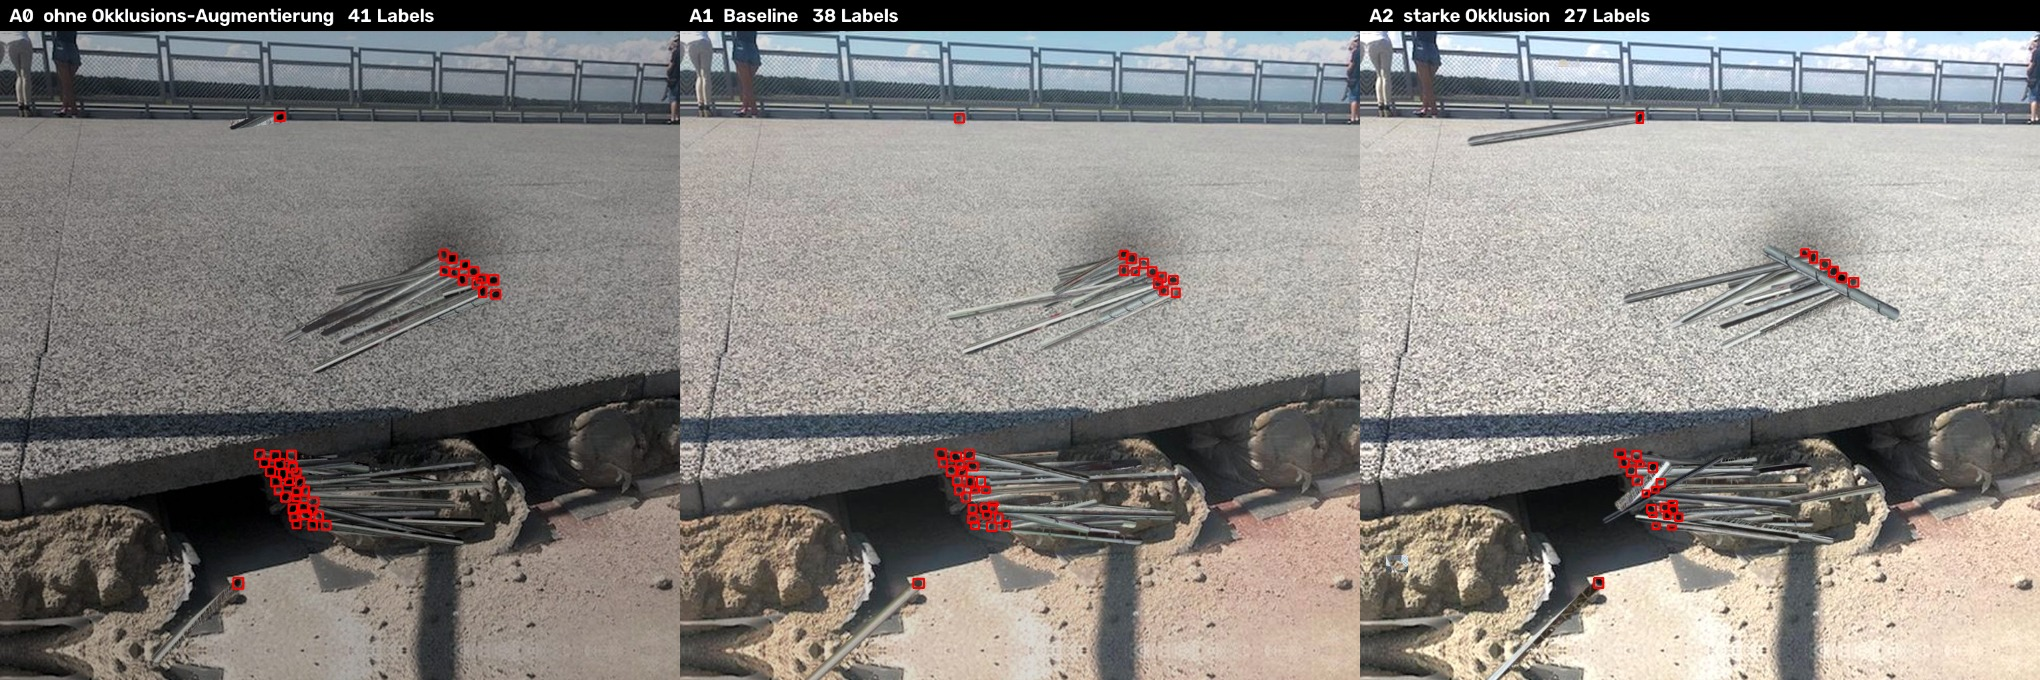
\includegraphics[width=\textwidth]{abbildungen/ablation_beispiele.jpg}
\caption[Die drei Ablationsarme]{Dasselbe Bild (identischer Seed) aus allen drei
Armen: A0 ohne Okklusion (links), A1 Baseline (Mitte), A2 starke Okklusion
(rechts). Die Objektpositionen sind identisch; es unterscheidet sich nur, wie
viel davon verdeckt ist -- und damit, wie viele Labels übrig bleiben.}
\label{abb:ablbeispiele}
\end{figure}

\subsection{Ergebnis}

\begin{table}[htbp]
\centering
\caption[Ergebnis der Okklusionsablation]{Ergebnis der Okklusionsablation,
nativer Maßstab. Alle sechs Metrikspalten sind über die drei Arme
\textbf{monoton}.}
\label{tab:ablergebnis}
\footnotesize
\resizebox{\textwidth}{!}{%
\begin{tabular}{@{}lrrrrrrr@{}}
\toprule
\textbf{Arm} & \textbf{Labels} &
\code{val} \mAPfifty{} & \code{val} \mAPall{} &
\code{test} \mAPfifty{} & \code{test} \mAPall{} & \code{test} F1 &
\code{test} Zählung \\
\midrule
A0 ohne     & 82\,950 & 0{,}888 & 0{,}606 & 0{,}899 & 0{,}418 & 0{,}896 & 77/86 \\
A1 Baseline & 68\,281 & 0{,}924 & 0{,}609 & 0{,}911 & 0{,}452 & 0{,}904 & 80/86 \\
A2 stark    & 55\,833 & \textbf{0{,}930} & \textbf{0{,}620} &
\textbf{0{,}919} & \textbf{0{,}454} & \textbf{0{,}910} & \textbf{81/86} \\
\bottomrule
\end{tabular}}
\end{table}

\begin{figure}[htbp]
\centering
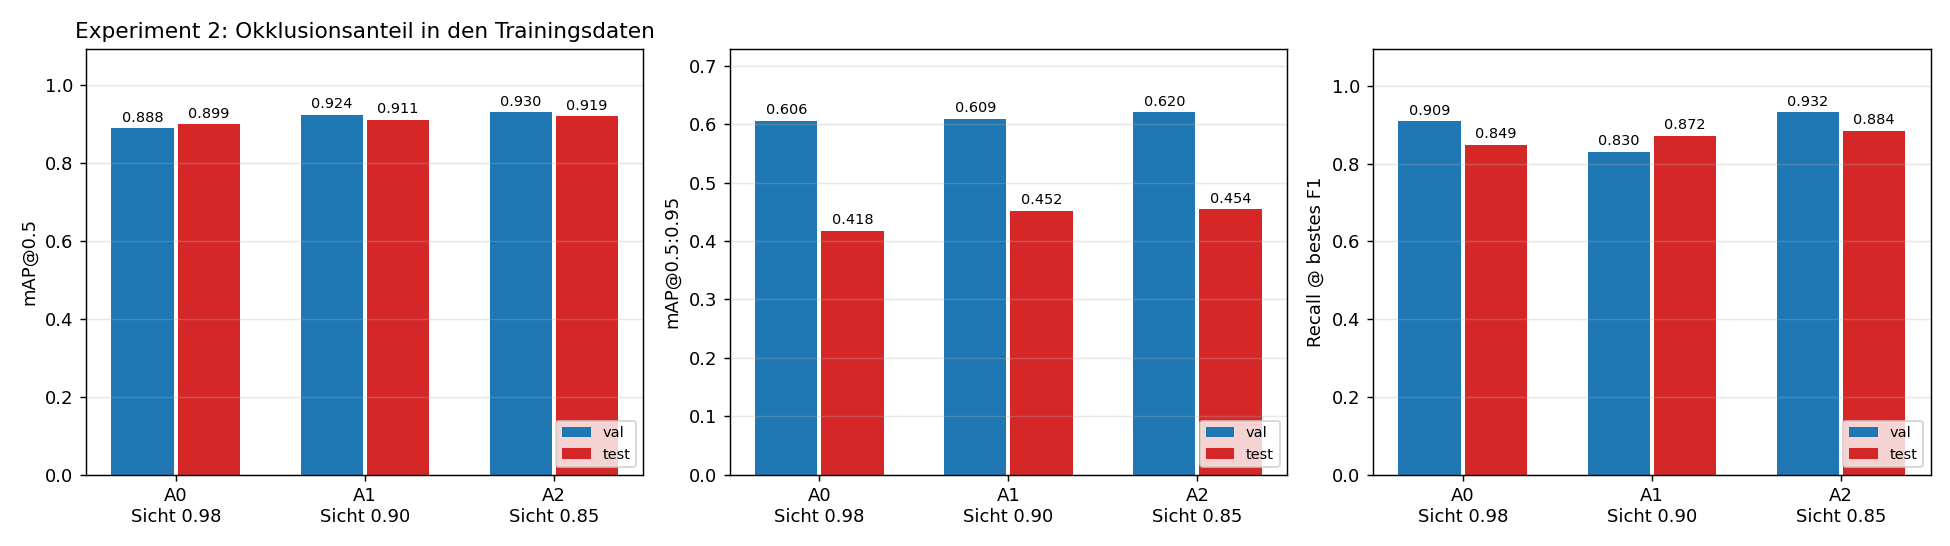
\includegraphics[width=\textwidth]{abbildungen/ablation.png}
\caption[Okklusionsablation]{Ergebnis der Okklusionsablation über die drei Arme.
Der Anstieg ist auf beiden Splits und in allen berichteten Metriken monoton.}
\label{abb:ablation}
\end{figure}

\absatz{Befund 1 -- der Effekt ist monoton.} Von A0 zu A2 steigen \mAPfifty{} um
2,0\PP{} und \mAPall{} um 3,6\PP{} auf dem unberührten Testbild. Der Anstieg
tritt in allen sechs Metrikspalten von Tabelle~\ref{tab:ablergebnis} und über
alle drei Stufen in derselben Richtung auf.

\absatz{Befund 2 -- der Gewinn entsteht \emph{gegen} einen Verlust an
Supervision.} A2 hat durch die stärkere Verdeckung \textbf{32,7\,\% weniger
Labels} als A0 (55\,833 gegen 82\,950 bei identischer Bildzahl und identischen
gerenderten Instanzen). Der Okklusionsvorteil überkompensiert also einen
deutlichen Verlust an Trainingssignal. Das ist der stärkste Einzelbeleg dafür,
dass die Okklusionsstufe kein Beiwerk ist: Wären die zusätzlichen Labels
wertvoller als die zusätzliche Schwierigkeit, müsste A0 gewinnen.

\absatz{Befund 3 -- ohne Verdeckung ist die Aufgabe zu leicht.} Ein zweiter
Befund steckt im Trainingsverlauf: \textbf{A0 erreichte sein bestes Modell
bereits in Epoche~3} und verbesserte sich in den folgenden 20 Epochen nicht mehr
(Early Stopping bei Epoche~23). A1 und A2 verbesserten sich bis zur letzten
Epoche~30 durchgehend. Ohne Verdeckung sättigt das Modell sofort und passt sich
danach nur noch an die synthetische Verteilung an -- dieselbe Schere wie in
Abschnitt~\ref{sec:trainingsverlauf}, nur früher einsetzend.

\absatz{Einordnung in die Literatur.} Der Befund ist mit den Ergebnissen zu
Cutout und Random Erasing verträglich \parencite{devries2017cutout,zhong2020erasing},
geht aber über sie hinaus: Dort wird Bildinhalt gelöscht und das Label
beibehalten, hier verdeckt ein Objekt mit eigener Textur, und das Label wird bei
zu starker Verdeckung entfernt. Die entstehenden Beispiele sind damit sowohl
schwierigere Positive als auch korrekte harte Negative -- letzteres ist bei
generischem Cutout nicht erreichbar. Das Ergebnis stützt zudem die Beobachtung
von \textcite{wang2017afastrcnn}, dass Okklusion für Detektoren ein wirksames
Trainingssignal ist.

\subsection{Einschränkungen dieses Experiments}
\label{sec:ableinschraenkung}

Die Einschränkungen sind erheblich und werden hier ausdrücklich genannt:

\begin{enumerate}
  \item \textbf{Der Effekt liegt innerhalb des Konfidenzintervalls.} Das
  Bootstrap-Intervall für \mAPfifty{} beträgt $\pm 0{,}05$ (\code{val}) bzw.\
  $\pm 0{,}04$ (\code{test}) und ist damit breiter als der gemessene Unterschied
  von 0,02--0,04 (Abschnitt~\ref{sec:bootstrap}). Belastbar ist nicht die
  einzelne Differenz, sondern die \emph{Konsistenz}: dieselbe Richtung in drei
  Metriken $\times$ zwei Splits $\times$ drei Stufen. Bei reinem Rauschen wäre
  eine solche durchgehende Monotonie unwahrscheinlich; ein formaler
  Signifikanznachweis ist mit je einem Bild pro Split aber nicht möglich.
  \item \textbf{Labelzahl und Okklusionsanteil sind nicht entkoppelt.} Mehr
  Verdeckung heißt zwangsläufig mehr verworfene Labels. Der Vergleich mischt
  also zwei Effekte, die sich hier zufällig gegenläufig verhalten. Ein saubereres
  Nachfolgeexperiment müsste die Bildzahl je Arm so anpassen, dass alle Arme
  gleich viele Labels enthalten.
  \item \textbf{A1 und A2 waren nach 30 Epochen nicht auskonvergiert.} Ihr
  Vorsprung könnte bei längerem Training größer werden -- die Aussage ist also
  konservativ, aber nicht abgeschlossen.
  \item \textbf{Eine Metrik ist nicht monoton.} \mAPseven{} auf \code{val}
  verläuft 0,812 / 0,760 / 0,775 und fällt damit aus dem Muster. Der Wert ist bei
  27\px{} großen Objekten besonders empfindlich gegenüber wenigen
  Boxabweichungen (Gleichung~\eqref{eq:ioushift}); die Aussage der Ablation
  betrifft das Finden der Objekte, nicht die Präzision der Boxen.
  \item \textbf{Ein Nebenbefund.} A1 und A2 (3000 Bilder, 30 Epochen) schlagen
  den Hauptlauf (6000 Bilder, bestes Modell aus Epoche~10) auf beiden Splits.
  Auch das liegt im Rauschen, deutet aber darauf hin, dass zusätzliche
  synthetische Bilder ab einer gewissen Menge nichts mehr bringen: Die Vielfalt
  ist durch die neun Ausschnitte begrenzt, nicht durch die Bildzahl.
\end{enumerate}

\section{Experiment 3: Modellfamilie}
\label{sec:modelle}

Dieses Experiment prüft nach, was Kapitel~\ref{kap:theorie} theoretisch
begründet: dass YOLO26 -- und insbesondere die Variante mit zusätzlichem
P2-Detektionskopf -- für kleine, dicht gepackte Objekte besser geeignet sein
sollte. Alle drei Läufe verwenden identisches Budget, identische
Hyperparameter und denselben Datensatz.

\begin{table}[htbp]
\centering
\caption[Modellfamilienvergleich]{Modellfamilienvergleich. Oben nativer
Maßstab, unten bei der je Modell auf \code{val} gewählten Auflösung
(\code{yolo11s}: 1920, \code{yolo26s}: 1600, \code{yolo26s-p2}: 1920). Die Wahl
erfolgte nach \mAPall{} und ausschließlich auf \code{val}; \code{test} blieb
unberührt.}
\label{tab:modelle}
\footnotesize
\resizebox{\textwidth}{!}{%
\begin{tabular}{@{}lrrrrrrr@{}}
\toprule
\textbf{Modell} & \textbf{Par.\ (M)} &
\code{val} \mAPfifty{} & \code{test} \mAPfifty{} & \code{test} \mAPseven{} &
\code{test} \mAPall{} & \code{test} F1 & \code{test} Zählung \\
\midrule
\multicolumn{8}{@{}l}{\itshape nativer Maßstab}\\
\code{yolo11s}    & 9{,}43 & 0{,}886 & 0{,}888 & 0{,}320 & 0{,}437 & 0{,}894 & 84/86 \\
\code{yolo26s}    & 9{,}95 & 0{,}931 & 0{,}905 & 0{,}333 & 0{,}427 & 0{,}888 & 83/86 \\
\code{yolo26s-p2} & 9{,}66 & 0{,}936 & \textbf{0{,}941} & \textbf{0{,}387} &
0{,}450 & \textbf{0{,}933} & 79/86 \\
\midrule
\multicolumn{8}{@{}l}{\itshape bei der auf \code{val} gewählten \code{imgsz}}\\
\code{yolo11s} (1920)    & 9{,}43 & 0{,}893 & 0{,}928 & -- & 0{,}448 & 0{,}917 & 82/86 \\
\code{yolo26s} (1600)    & 9{,}95 & 0{,}939 & 0{,}905 & -- & 0{,}427 & 0{,}888 & 83/86 \\
\code{yolo26s-p2} (1920) & 9{,}66 & \textbf{0{,}940} & \textbf{0{,}947} & -- &
0{,}449 & \textbf{0{,}934} & 81/86 \\
\bottomrule
\end{tabular}}
\end{table}

\absatz{Interpretation.} Die theoretische Erwartung bestätigt sich: Bei
praktisch identischer Parameterzahl erreicht \code{yolo26s-p2} auf dem
unberührten Testbild \mAPfifty{} = 0,941 statt 0,888. Der Gewinn entsteht dabei
\emph{nicht} über die Boxpräzision: Die mittlere Treffer-IoU sinkt sogar leicht
(0,748 auf 0,728). Er entsteht über die Trennung von Objekt und Hintergrund --
die Precision am Betriebspunkt steigt von 0,905 auf 0,975 bei ebenfalls leicht
höherem Rückruf (0,884 auf 0,895). Das ist mit der Argumentation aus
Abschnitt~\ref{sec:ioukleinobjekt} konsistent: Ein zusätzlicher P2-Kopf mit
Stride~4 senkt die Auflösungsgrenze, an der ein Objekt überhaupt detektierbar
ist; er macht aber die Boxregression bei 20\px{}-Objekten nicht genauer. Der
Preis ist der Speicherbedarf: Die P2-Variante belegte im Training rund die
2,6-fache GPU-Speichermenge.

\absatz{Ein Vorbehalt für die Zählanwendung.} Der Vorteil in \mAPfifty{} setzt
sich nicht in einen besseren Zählfehler um: Am F1-optimalen Betriebspunkt zählt
\code{yolo26s-p2} auf \code{test} 79 statt 86 Objekte (Fehler 8,1\,\%),
\code{yolo11s} dagegen 84 (2,3\,\%). Die Ursache ist die Schwellenwahl: Das
F1-Optimum von \code{yolo26s-p2} liegt bei $c^* = 0{,}379$ gegenüber
$0{,}263$, tauscht also Rückruf gegen Precision. Da F1 beide Fehlerarten
gleich gewichtet, der Zählfehler sich aber aus ihrer \emph{Differenz} ergibt,
sind die beiden Optima nicht identisch. Für eine Zählanwendung ist der
Betriebspunkt daher direkt auf den Zählfehler zu optimieren und nicht auf F1 --
eine Einsicht, die für alle Modelle gilt und in dieser Arbeit bewusst nicht
umgesetzt wurde, weil eine auf \code{val} kalibrierte Zählschwelle die
Aussagekraft der \code{test}-Zahlen geschwächt hätte.

\absatz{Konsequenz und ehrliche Einordnung.} Die Wahl der Modellfamilie war
damit die schwächste Einzelentscheidung der Arbeit -- sie war zunächst
konservativ und unbelegt getroffen. \code{yolo11s} bleibt als dokumentierte
Baseline stehen, weil auf ihr die Experimente~1 und 2 gerechnet wurden; für einen
produktiven Einsatz wäre \code{yolo26s-p2} zu wählen. Für die
Augmentierungsergebnisse dieser Arbeit ändert das nichts: Alle drei Modelle haben
dieselben Strides auf P3/P4/P5, und die Ablation vergleicht Datensätze bei
identischem Modell.

\section{Statistische Belastbarkeit}
\label{sec:bootstrap}

Nach Befund~10 liegt je Split nur \emph{ein} Bild vor. Eine mAP-Angabe auf 88
Objekten ist eine Punktschätzung mit erheblicher Streuung, und ein gewöhnlicher
Bootstrap über Bilder ist nicht möglich. Verwendet wird daher ein
\textbf{räumlicher Block-Bootstrap}: Das Bild wird in Kacheln zerlegt, und es
wird über Kacheln mit Zurücklegen neu gezogen (400 Wiederholungen). Das Verfahren
entspricht dem Block-Bootstrap für abhängige Beobachtungen
\parencite{kuensch1989,efron1993}; die Blockbildung ist nötig, weil benachbarte
Objekte nicht unabhängig sind -- sie teilen Beleuchtung, Schärfe und
Verdeckungssituation.

\begin{table}[htbp]
\centering
\caption[Bootstrap-Konfidenzintervalle]{Bootstrap-Konfidenzintervalle für
\mAPfifty{}, 400 Wiederholungen über räumliche Kacheln.}
\label{tab:bootstrap}
\small
\begin{tabular}{@{}lrrrr@{}}
\toprule
\textbf{Split} & \textbf{Mittel} & \textbf{Std} & \textbf{95\,\%-KI} &
\textbf{Kacheln} \\
\midrule
\code{val}  & 0{,}892 & 0{,}051 & $[0{,}766;\ 0{,}965]$ & 23 \\
\code{test} & 0{,}911 & 0{,}036 & $[0{,}844;\ 0{,}974]$ & 25 \\
\bottomrule
\end{tabular}
\end{table}

Die Intervalle sind breit -- rund $\pm 0{,}05$ bzw.\ $\pm 0{,}04$. Alle in
diesem Kapitel berichteten Unterschiede unterhalb dieser Größenordnung sind
daher als Hinweis und nicht als Nachweis zu lesen. Das betrifft die
Okklusionsablation (Abschnitt~\ref{sec:ableinschraenkung}) und den
Modellvergleich; es betrifft \emph{nicht} den Auflösungseffekt aus
Abschnitt~\ref{sec:imgsz}, dessen Größe von 47\PP{} das
Intervall um ein Vielfaches übersteigt.

\section{Fehleranalyse}
\label{sec:fehleranalyse}

Aus den Qualitativbildern (Abbildung~\ref{abb:qualitativ}) lassen sich die
Fehler nach Ursache ordnen.

\absatz{Falsch-Negative} treten fast ausschließlich auf bei
\begin{itemize}
  \item sehr kleinen Objekten am linken Bildrand von \code{test}
  (12--15\px{}) -- also am unteren Rand der in
  Gleichung~\eqref{eq:effskala} abgedeckten Größenspanne,
  \item stark verdeckten Enden tief im Stapel -- also genau dort, wo die
  Pipeline nach Abschnitt~\ref{sec:sichtbarkeit} auch kein Label mehr vergäbe,
  \item Enden ohne sichtbaren hellen Kranz, die vollständig im Schatten liegen.
  Dies ist der Fehlertyp, der auf die verbleibende Domänenlücke zurückgeht: Alle
  vier Clean Plates sind bei diffusem Licht aufgenommen
  (Abschnitt~\ref{sec:hintergruende}).
\end{itemize}

\absatz{Falsch-Positive} haben auf den beiden Bildern \emph{unterschiedliche}
Ursachen, und die Unterscheidung ist nicht kosmetisch. Auf \code{val} haben 9 der
11 Falsch-Positiven keinerlei Überlappung mit einer Ground-Truth-Box; ein Teil
von ihnen sitzt auf erkennbaren Rohröffnungen, die in der Annotation fehlen. Bei
88 handannotierten Objekten schlägt jede fehlende Annotation mit etwa 1,1\PP{}
Precision zu Buche -- die berichteten Precision-Werte sind daher eher eine
\textbf{Untergrenze} als eine Punktschätzung. Die übrigen entstehen an dunklen
Löchern im Maschendraht und an Schattenspalten zwischen Rohren, genau die
Strukturen, gegen die die Negativbilder aus Abschnitt~\ref{sec:negative}
gerichtet sind; dass sie dort noch auftreten, spricht dafür, dass deren Anteil
von 9,7\,\% eher an der Untergrenze des Sinnvollen liegt.

Auf \code{test} liegt der Fall völlig anders: Dort sind \textbf{sechs der acht
Falsch-Positiven} Detektionen, die auf einem annotierten Objekt sitzen und die
Zuordnungsschwelle nur knapp verfehlen (IoU 0,401 bis 0,497, in zwei Fällen um
weniger als 0,005). Sie erscheinen im Qualitativbild als rote Box direkt neben
oder in einer blauen -- dasselbe Objekt wird gleichzeitig als Falsch-Positiv und
als Falsch-Negativ gezählt. Der nächste Abschnitt geht dem nach.

\section{Ein systematischer Größenversatz der Boxen}
\label{sec:boxversatz}

Eine Detektion gilt nur als Treffer, wenn ihre IoU mit der Ground-Truth-Box
mindestens 0,5 beträgt; liegt sie darunter, bleibt die Detektion unzugeordnet und
die Ground-Truth-Box unbedient. Auf \code{test} ergeben sich dadurch aus sechs
gefundenen Objekten zwölf Fehler. Senkt man allein die Zuordnungsschwelle von
0,50 auf 0,40, so ergeben sich 81 Treffer, 2 Falsch-Positive und 5
Falsch-Negative statt 75/8/11.

\begin{table}[htbp]
\centering
\caption[Größenversatz der Boxen]{Oben: Vergleich der vorhergesagten mit der
annotierten Boxgröße für alle Detektionen, die eindeutig auf einem annotierten
Objekt sitzen ($\mathrm{IoU} > 0{,}3$); als Boxgröße dient
$\sqrt{\text{Fläche}}$. Unten: Sensitivitätsrechnung mit um den medianen
Fehlbetrag je Seite aufgeweiteten Boxen -- \emph{kein} Ergebnis eines neuen
Trainings, sondern eine Obergrenzenschätzung.}
\label{tab:boxversatz}
\footnotesize
\begin{tabular}{@{}llrrrrr@{}}
\toprule
\multicolumn{7}{@{}l}{\itshape gemessener Versatz}\\
\textbf{Split} & & \textbf{Paare} & \textbf{Objekt-\Oe} &
\textbf{pred/GT} & \textbf{GT $-$ pred} & \textbf{Zentrumsversatz} \\
\midrule
\code{test} (real)        & &   82 & 22,3\px & 0,884 & $+2{,}53$\px & 0,049\,\Oe \\
\code{val} (real)         & &   75 & 27,5\px & 0,961 & $+1{,}16$\px & 0,054\,\Oe \\
\code{sval} (synthetisch) & & 1064 & 22,0\px & \textbf{1,012} & $-0{,}29$\px & -- \\
\midrule
\multicolumn{7}{@{}l}{\itshape Sensitivitätsrechnung}\\
 & & \mAPfifty{} & \mAPseven{} & \mAPall{} & \textbf{bestes F1} &
\textbf{mittl.\ IoU} \\
\midrule
\code{test} & unverändert       & 0,887 & 0,320 & 0,437 & 0,894 & 0,748 \\
\code{test} & Boxen aufgeweitet & \textbf{0,951} & \textbf{0,714} &
\textbf{0,604} & \textbf{0,959} & \textbf{0,805} \\
\code{val}  & unverändert       & 0,886 & 0,793 & 0,597 & 0,862 & 0,824 \\
\code{val}  & Boxen aufgeweitet & 0,886 & 0,812 & 0,622 & 0,862 & 0,835 \\
\bottomrule
\end{tabular}
\end{table}

\begin{figure}[htbp]
\centering
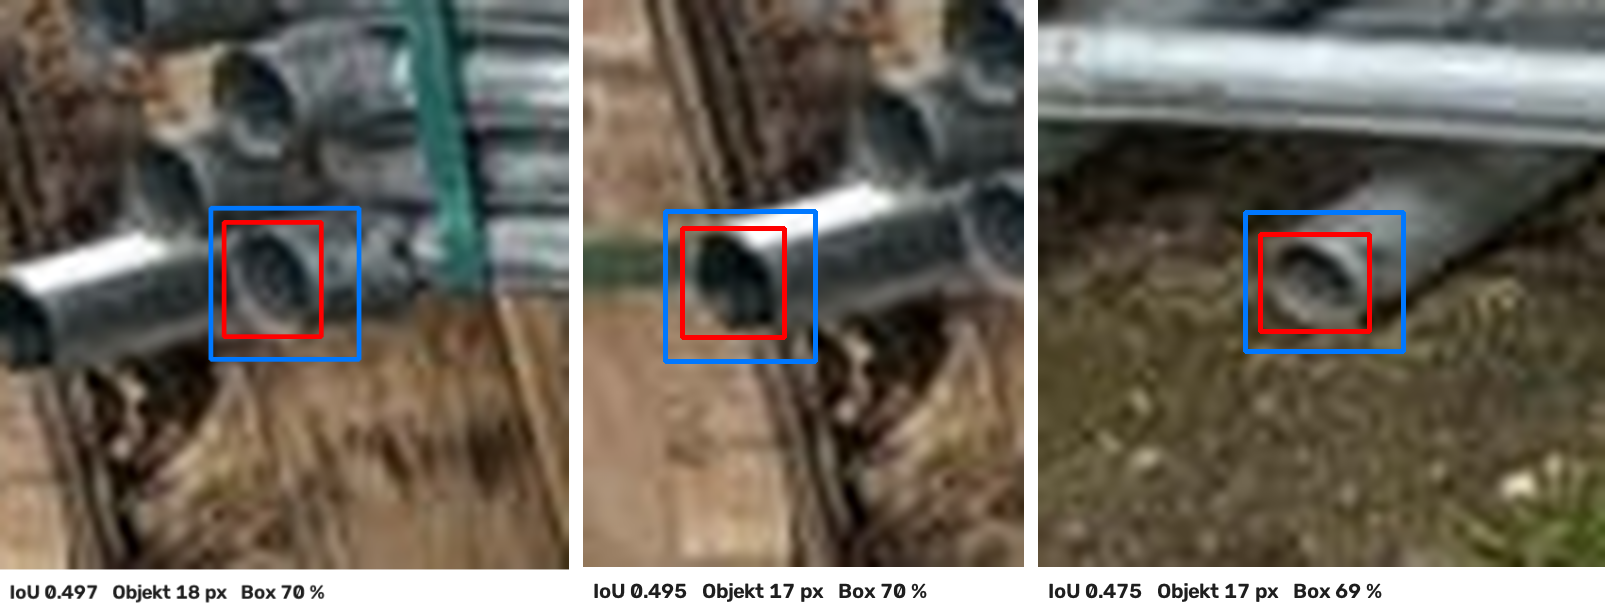
\includegraphics[width=\textwidth]{abbildungen/boxversatz.png}
\caption[Rote und blaue Box am selben Objekt]{Drei der sechs betroffenen Stellen
aus dem Testbild, neunfach vergrößert. Blau die Handannotation, rot die
Detektion. Alle drei Objekte sind gefunden, die vorhergesagte Box umfasst aber
nur etwa 70\,\% der annotierten Kantenlänge; die IoU bleibt damit knapp unter der
Zuordnungsschwelle 0,5, und dasselbe Objekt zählt als Falsch-Positiv \emph{und}
als Falsch-Negativ.}
\label{abb:boxversatz}
\end{figure}

Tabelle~\ref{tab:boxversatz} zeigt die Ursache. Auf dem synthetischen Split
trifft das Modell die Boxgröße auf 1\,\% genau, auf den realen Bildern liegt sie
4\,\% (\code{val}) bzw.\ 12\,\% (\code{test}) darunter. Der Versatz ist in
\emph{absoluten} Pixeln annähernd konstant und trifft deshalb die kleinsten
Objekte am härtesten (Verhältnis 0,830 bei Objekten unter 18\px{} gegen 0,894
über 26\px{}); der Zentrumsversatz bleibt mit 0,05 Objektdurchmessern im Bereich
der Annotationsgenauigkeit. Es ist also ein Größen-, kein Positionsfehler.

Weil das Modell auf dem synthetischen Split die Boxgröße nahezu exakt
reproduziert, liegt die Ursache nicht in der Boxregression, sondern in der
\emph{Labelkonvention}: Die Generatorboxen folgen der $\alpha > 0{,}5$-Kontur der
Alphamaske (Abschnitt~\ref{sec:sichtbarkeit}), die Handannotation umschließt das
Objekt großzügiger. Anforderung~A5 -- identische Labeldefinition in Quelle und
Ziel -- ist damit nur \emph{annähernd} erfüllt, mit einem messbaren Restversatz
von 1,2 bis 2,5\px. Ein Teil davon ist zugleich echte
Lokalisierungsschwierigkeit: Betroffen sind die kleinsten und kontrastärmsten
Objekte, bei denen sich die Detektion auf die dunkle Bohrung zusammenzieht,
während die Annotation den hellen Kranz einschließt.

Die Sensitivitätsrechnung im unteren Teil von Tabelle~\ref{tab:boxversatz}
schätzt die Größenordnung: Auf \code{test} steigt \mAPseven{} von 0,320 auf 0,714
und \mAPall{} von 0,437 auf 0,604, auf \code{val} bewegt sich entsprechend wenig.
Die berichteten Lokalisierungsmetriken auf \code{test} sind damit
\textbf{pessimistisch} -- sie messen zu einem erheblichen Teil eine
Konventionsdifferenz. Für \mAPfifty{}, das F1 und den Zählfehler bleibt der
Effekt klein. Die Korrektur ist einfach und sollte vor jeder weiteren
Optimierung erfolgen: Boxschwelle im Generator von $\alpha > 0{,}5$ herabsetzen
oder die fertige Box um etwa 1\px{} je Seite aufweiten.

\chapter{Diskussion und Fazit}
\label{kap:diskussion}

\section{Was ist belegt, was ist nur begründet?}
\label{sec:tragend}

Kapitel~\ref{kap:pipeline} hat gezeigt, dass die Pipeline die Anforderungen A1
--A6 erfüllt. Das ist eine Aussage über den Entwurf, nicht über die Wirkung.
Für eine belastbare Bilanz ist zwischen Entscheidungen zu unterscheiden, deren
Nutzen \emph{gemessen} wurde, und solchen, die lediglich \emph{begründet} sind.
Von stark nach schwach geordnet ergeben sich vier Stufen.

\textbf{Abliert}, also in eigenen Trainingsläufen geprüft, die sich nur in
dieser einen Größe unterscheiden, ist allein das Bündel der
Einbettungsmaßnahmen gegen S1--S5 samt Schlagschatten
(Abschnitt~\ref{sec:ablationC}); welche Einzelmaßnahme darin wie viel trägt,
ist offen. \textbf{Ohne Neutraining gemessen} sind die Inferenzparameter
(Abschnitt~\ref{sec:imgsz}). Nur die Auflösung zeigt dabei einen Effekt über
dem Bootstrap-Intervall; NMS-Schwelle und Test-Time-Augmentation bleiben beim
Ende-zu-Ende-Kopf wirkungslos, und \code{max\_det} verändert ab 100 den
Betriebspunkt und ab 200 auch \mAPfifty{} nicht mehr.
\textbf{An der erzeugten Verteilung kalibriert} sind Objektgrößenbereich,
Ovalisierungsanteil, Gitterabstände, die Basisgröße je Cluster, das
Tiefenmodell 75/25 und die Randregel: Die erzeugte Statistik trifft die reale
(Tabelle~\ref{tab:kalibrierung}), ihr Nutzen für die Detektion ist damit aber
nicht gemessen. \textbf{Nur begründet} sind alle übrigen Entscheidungen,
darunter die Herkunft der Okkluder, die Matting-Schwelle, Gamma, HSV, Mulde,
globale Bildstufe, Negativbildanteil sowie Dellen- und Perspektivanteil.

\absatz{Bilanz der Begründungen.} Die Zielsetzung hatte drei zulässige Quellen
festgelegt und für alles andere die Kennzeichnung als Annahme verlangt.
Tabelle~\ref{tab:parameter} dokumentiert 37 Transformationen mit 44
Parameterwerten: 7 sind an den Realdaten gemessen, 8 literaturgestützt, 2
physikalisch begründet, 11 gemischt und \textbf{16 ausdrücklich als Annahme
gekennzeichnet}. Rund 64\,\% sind damit auf eine der drei zulässigen Quellen
zurückgeführt -- die elf gemischten allerdings nur zur Hälfte --, 36\,\% sind
Annahmen. Diese Bilanz ist nicht nebensächlich: Bei rein synthetischen Trainingsdaten
ist die Liste dieser 44 Werte die vollständige Beschreibung der
Trainingsverteilung.

Gemessen an diesen 44 Werten ist ein einziges abliertes Bündel wenig. Die
Begründungen tragen den Entwurf, experimentell belegt ist daraus ein
Punkt. Er ist allerdings nicht beliebig gewählt, denn er betrifft das
Leitprinzip der Pipeline.

\absatz{Eine Größe verbindet fünf Entscheidungen.} Rückblickend steht eine
einzige Kenngröße hinter dem größten Teil der Arbeit: die effektive Objektgröße
$d_{\text{eff}} = d \cdot M/N$ aus Gleichung~\eqref{eq:deff}, bezogen auf den
Stride $S$ der feinsten Detektionsebene. Aus diesem Verhältnis folgen
\emph{erstens} die Kalibrierung des Generators auf 12--44\px, weil die
Realobjekte 6--36\px{} groß sind (Abschnitt~\ref{sec:valtest}),
\emph{zweitens} die Trainingsauflösung 1024, weil sie der Leinwandgröße
entspricht und die kalibrierte Verteilung damit unskaliert beim Netz ankommt
(Abschnitt~\ref{sec:trainingsaufbau}), \emph{drittens} die Wahl des P2-Kopfes,
weil er $S$ von 8 auf 4 senkt und die kritische Größe $S\sqrt{2}$ damit unter
alle auftretenden Objektgrößen schiebt (Abschnitt~\ref{sec:trainingsaufbau}),
\emph{viertens} die Inferenzauflösung (Abschnitt~\ref{sec:imgsz}) und
\emph{fünftens} die Erklärung des größten gemessenen Einzeleffekts, des
Einbruchs auf \mAPfifty{} \zswValNiedrig{} bei \code{imgsz}~640, den
Abschnitt~\ref{subsec:kleine-objekte} vorhergesagt hatte, bevor er gemessen
wurde. Diese Kette ist das methodisch belastbarste Ergebnis der Arbeit: Aus
einer einzigen Größe folgen fünf Entscheidungen, und eine daraus abgeleitete
Vorhersage ist eingetroffen.

\section{Grenzen und nächste Schritte}
\label{sec:grenzen}

\absatz{Grenzen der Pipeline.} \emph{(1)} Nur sechs Quellobjekte aus einer
einzigen Aufnahme -- jedes erscheint rund 22\,700-mal als gelabeltes Objekt.
Die photometrische und geometrische Streuung mildert das, hebt es aber nicht
auf; Augmentierung erzeugt keine neue Information über die Objektklasse. Keines
der sechs zeigt eine mit Laub oder Rost gefüllte Bohrung, und genau solche
Enden übersieht das Modell auf \code{val} (Abschnitt~\ref{sec:bootstrap}). Auf
die geringe Formvielfalt stützt sich auch die Wahl der Modellgröße
\enquote{s} (Abschnitt~\ref{sec:trainingsaufbau}); dass mehr Kapazität hier vor
allem auswendig lernen würde, ist plausibel \parencite{zhang2017rethinking},
aber nicht gemessen. \emph{(2)} Nur diffuses Licht im Quellmaterial: Harte
Schlagschatten, Gegenlicht, Nässe und Schnee fehlen vollständig und werden nur
approximativ über die globale photometrische Stufe angenähert. Ob das die
Detektion beeinträchtigt, zeigt die Fehleranalyse nicht; ihr zweiter Fehlertyp
geht auf die Erscheinung der Rohrenden selbst zurück. \emph{(3)} Reflect-Padding erzeugt Spiegelsymmetrie, wenn ein
Hintergrund für den gewünschten Zoom zu klein ist; eine spiegelsymmetrische
Bildhälfte ist selbst ein erkennbares Merkmal, die Maßnahme gegen Signatur~S1
erzeugt damit eine schwächere neue Auffälligkeit. \emph{(4)} Die Schaftrichtung ist an der
Säulenrichtung des Clusters kalibriert, nicht an der Rohrrichtung des
Hintergrunds. In 19,4\,\% der Cluster auf Clean Plates kreuzt der Schaft die
Hintergrundrohre deshalb unter mehr als $60^\circ$, betroffen sind 22,0\,\% der
erzeugten Bilder (\code{src/schaftwinkel.py}), obwohl real alle Rohre eines
Stapels parallel liegen. Ein Angleich wäre
mit geringem Aufwand möglich, weil die dominante Hintergrundrichtung gemessen
vorliegt (\code{src/occluders.py}).

\absatz{Grenzen der Bewertung.} Die schwerwiegendste methodische Schwäche liegt
nicht in der Pipeline, sondern in der Bewertung: \emph{je ein Bild} pro Split.
Daraus folgen breite Konfidenzintervalle: $[\zbootValLo;\,\zbootValHi]$ auf
\code{val} und $[\zbootTestLo;\,\zbootTestHi]$ auf \code{test}, also drei bis
vier Prozentpunkte Halbbreite -- Unterschiede unterhalb dieser Größe sind nicht
entscheidbar; beide Bilder zeigen dieselbe Objektart bei ähnlichem
Wetter, die Ergebnisse sagen also nichts über andere Zaunhersteller,
Rohrdurchmesser oder Lichtsituationen. Schließlich wird \code{val} doppelt
verwendet -- für die Modellauswahl \emph{und} für die Wahl der
Inferenzauflösung. \code{val} ist damit kein unabhängiger Bewertungssplit
mehr.

\absatz{Quellmaterial und Bewertungsdaten.} Bildinhalt teilen Quellmaterial und
Bewertungsbilder nicht (Abschnitt~\ref{sec:valtest}), unabhängig sind sie aber
nicht. Alle sechs Objektausschnitte und zwei der vier Clean Plates stammen aus
derselben Aufnahmeserie wie \code{val}, aufgenommen innerhalb von 20 Sekunden
am selben Ort mit derselben Kamera. Die \code{val}-Zahlen messen deshalb auch,
wie gut das Modell auf eine Szene überträgt, aus der sein Quellmaterial stammt.
Außerdem ist die Labelstatistik beider Bilder in die Kalibrierung eingegangen,
am deutlichsten bei der unteren Größengrenze von 12\px, dem 5\,\%-Quantil von
\code{test} (Befund~5). Streng getrennt wäre eine Kalibrierung allein an
\code{val}; die untere Grenze läge dann bei 19\px, und die kleinen Objekte in
\code{test} deckte nur noch die Trainingsskalierung ab. \code{test} ist damit
der einzige Split, der einen anderen Stapel zeigt als das Quellmaterial und
dessen Ergebnisse in keine Entscheidung eingehen; die
belastbaren Zahlen sind die \code{test}-Zahlen.

\absatz{Grenzen der Ablation.} Drei Vorbehalte bleiben. \emph{Erstens} das
reduzierte Budget: 3000 Bilder und 30 Epochen sind aus der Rechenzeit gewählt,
nicht aus einem Konvergenzkriterium. Es ist für beide Arme gleich und kann
den Vergleich deshalb nicht verzerren, begrenzt aber die absolute Höhe der
Zahlen; ein Effekt, der sich erst nach 60 Epochen zeigte, bliebe unentdeckt.
\emph{Zweitens} je ein Lauf pro Arm: Ohne Wiederholung mit verschiedenen
Trainings-Seeds ist die Streuung des Trainings selbst unbekannt und von der
Wirkung des Datensatzes nicht zu trennen, zumal der Effekt nur auf einem der
beiden Bilder größer ist als die Messunsicherheit. Das ist die gewichtigste
Einschränkung, und sie ist mit Rechenzeit behebbar: Drei Seeds je Arm wären
sechs statt zwei Läufen. \emph{Drittens} ist die Ablation ein \emph{Eingriff
in eine Richtung}: Sie
zeigt die Folgen einer Verschlechterung, nicht den Ertrag eines besseren
Entwurfs derselben Stufen.

\absatz{Nächste Schritte.} Jede der genannten Grenzen hat eine Gegenmaßnahme;
nach erwartetem Nutzen geordnet:

\begin{enumerate}[itemsep=3pt,leftmargin=1.6em]
  \item \textbf{Labelkonvention angleichen.} Eine geänderte Boxschwelle im
  Generator genügt, und die Sensitivitätsrechnung lässt auf \code{test} rund
  \zsensTestGain{} Punkte \mAPseven{} erwarten; das ist der mit geringstem Aufwand erreichbare Gewinn dieser Liste, anzugehen vor jeder weiteren Optimierung.
  \item \textbf{Mehr Bewertungsdaten und mehrere Seeds.} Zehn bis zwanzig
  annotierte Realbilder aus Aufnahmen, aus denen kein Quellmaterial stammt,
  würden die Konfidenzintervalle auf ein Maß bringen, bei
  dem auch kleinere Differenzen entscheidbar wären; drei Trainings-Seeds je Arm
  trennen zusätzlich die Streuung des Trainings von der Wirkung des Datensatzes.
  Zusammen sind das die beiden Punkte, die aus einem Hinweis einen Nachweis
  machen.
  \item \textbf{Das Bündel der Ablation auflösen.} Wie sich der Effekt auf die
  einzelnen Einbettungsmaßnahmen verteilt, ist offen. Je ein Lauf ohne Farb-,
  Rausch- und Unschärfeangleich, ohne weiche Alphakante und ohne JPEG-Durchlauf
  schlüsselt ihn auf, mit dem Sim-to-Real-Abstand als Zielgröße. Schon zwei Arme
  trennen Abkürzung und Domänenlücke (Abschnitt~\ref{sec:ablationC}): Verliert
  der Arm nur mit harter Kante mehr als der nur ohne photometrischen Angleich,
  spricht das für die Abkürzung. Auf dieselbe Weise ließen sich der
  Verdeckungs\emph{grad} und die \emph{Herkunft} der Okkluder prüfen, die
  bisher nur begründet sind.
  \item \textbf{Breiteres Quellmaterial.} Objektausschnitte aus mehreren
  Aufnahmen, darunter Enden mit gefüllter oder verschmutzter Bohrung, die die
  Fehleranalyse als den Fehlertyp ausweist, der nicht auf Objektgröße
  zurückgeht; dazu Clean Plates bei harter Sonne, Gegenlicht und Nässe.
\end{enumerate}

\section{Fazit}

Ein ausschließlich auf synthetischen Bildern trainierter Detektor erreicht auf
zwei echten Aufnahmen \mAPfifty{} von \textbf{\zrefValMap} und
\textbf{\zrefTestMap} bei einem besten $F_1$ von \zrefValFf{} und \zrefTestFf;
auf \code{test}, das weder im Quellmaterial vorkommt noch zur Modellauswahl
dient, zählen von \znPredTest{} Detektionen nur \zfpTest{} als falsch-positiv,
\zfpDoppelTest{} davon als zweite Box auf einer bereits erkannten Stirnfläche. Für
eine Anwendung, für die kein einziges handannotiertes Trainingsbild existiert,
ist das ein tragfähiges Ergebnis.

Methodisch tragen drei Einsichten:

\begin{enumerate}[itemsep=3pt]
  \item \textbf{Bei rein synthetischen Trainingsdaten ist die Pipeline die
  Hypothese.} Jede Entscheidung über eine Transformation ist eine Aussage
  darüber, welche Invarianzen in der Zieldomäne gelten. Die Begründungspflicht
  (Messung, physikalische Randbedingung, Literatur oder ausgewiesene Annahme)
  ist deshalb keine Formalität, sondern das eigentliche Handwerk. Sie hat
  zudem einen Nebeneffekt, den diese Arbeit nutzt: Wer jede Begründung
  ausschreibt, macht sichtbar, welche davon noch nie geprüft wurde.
  \item \textbf{Sorgfalt beim Einfügen ist kein Feinschliff, und keine
  synthetische Kennzahl zeigt an, wenn sie fehlt.} Werden die Maßnahmen gegen
  die Signaturen S1--S5 abgeschaltet, ändert sich \mAPfifty{} auf dem
  Testbild um $\zablCTestGap$\PP, auf dem \emph{eigenen} synthetischen Split
  desselben Arms aber nur um $\zablCSvalGap$\PP; auf dem zweiten Realbild
  bleibt der Unterschied innerhalb der Messunsicherheit. Der Schaden entsteht
  ausschließlich in der Übertragung und ist an den synthetischen Daten
  unsichtbar. Wer eine Copy-Paste-Pipeline an ihren eigenen Bildern misst,
  misst die falsche Größe; nötig ist ein beschrifteter realer Split, und sei
  es ein einziges Bild.
  \item \textbf{Auflösung dominiert, und die Labelkonvention ist Teil des
  Messinstruments.} Zwischen \code{imgsz}~640 und dem Optimum liegen
  \zswValGain\PP{} \mAPfifty, mehr als das Vierfache des Effekts der
  Einbettung. Ein systematischer Größenversatz von rund zwei Pixeln
  zwischen Generatorlabel und Handannotation verschiebt außerdem \mAPseven{}
  auf dem Testbild von \zsensTestMapSOrig{} auf \zsensTestMapSNeu, ohne dass
  sich am Modell etwas ändert. Wer Lokalisierungsmetriken bei 20\px-Objekten berichtet, muss beide
  Größen zuerst kennen.
\end{enumerate}


% ------------------------------- Verzeichnisse ----------------------------
\printbibliography[heading=bibintoc,title={Literaturverzeichnis}]

\appendix
\chapter{Anhang}
\label{kap:anhang}

\section{Reproduktion}

Alle Messwerte dieser Arbeit lassen sich mit der folgenden Befehlsfolge
erzeugen. Die Nummerierung entspricht Tabelle~\ref{tab:kette}.

\begin{footnotesize}
\begin{verbatim}
# 0  Sichtung (erzeugt alle Messwerte aus Kapitel 4)
python src/analyze_data.py

# 1  Objektausschnitte freistellen  -> assets/masks/, docs/matting_check.png
python src/matting.py

# 2  Okkluder-Bibliothek            -> assets/bars/, docs/bars_check.png
python src/occluders.py

# 3  Trainingsdaten                 -> synth/train/ + generation_report.json
python src/generate.py --out synth/train --n 6000 --seed 1 --preview 8
python src/generate.py --out synth/sval  --n  400 --seed 99

# 4  Training
python src/train.py --name baseline

# 5  Auswertung (nativer Massstab, eigene Metriken + Kreuzvergleich)
python src/evaluate.py --weights runs/baseline/weights/best.pt \
    --splits val,test --crosscheck --vis docs/qual_SPLIT_NAME.jpg \
    --out docs/experiments/final_eval.json

# 6  Experimente
python src/experiment.py infer          # Experiment 1  (Abschnitt 7.4, 7.5)
python src/experiment.py ablation-data  # Experiment 2  (Abschnitt 7.6)
python src/experiment.py ablation-train
python src/experiment.py ablation-eval
python src/train.py --name yolo26s    --model yolo26s.pt
python src/train.py --name yolo26s_p2 --model yolo26s-p2.yaml \
    --pretrained yolo26s.pt
python src/experiment.py models         # Experiment 3  (Abschnitt 7.7)

# 7  Diagramme und Tabellen
python src/report.py

# 8  Abbildungen dieses Dokuments aufbereiten
python paper/tools/abbildungen_vorbereiten.py
python paper/tools/fig_boxversatz.py
\end{verbatim}
\end{footnotesize}

\section{Umgebungshinweis}

Eine Einschränkung der Ausführungsumgebung ist für die Reproduktion relevant und
wird hier festgehalten, weil sie einen Trainingsparameter erzwingt: In der
verwendeten Kombination aus \code{opencv-python}~5.0.0.93 und \code{torch}~2.13
verklemmt sich der fork-basierte DataLoader der Werkzeugkette reproduzierbar beim
ersten Batch, sobald \code{workers > 0} gesetzt ist. Getestet und jeweils
erfolglos: \code{cv2.setNumThreads(0)}, deaktiviertes OpenCL, gesetzte
\code{OMP\_NUM\_THREADS}- und \code{MKL\_NUM\_THREADS}-Grenzen sowie die
Startmethode \code{spawn}. Das Training läuft deshalb mit \code{workers=0} und
hält stattdessen alle dekodierten Bilder im Arbeitsspeicher
(\code{cache='ram'}, 6000 Bilder $\approx$ 18\,GB). Der Cache wird von einem
Thread-Pool gefüllt und ist von dem Deadlock nicht betroffen; der Wegfall der
JPEG-Dekodierung im Hauptprozess ist dort der größte einzelne Zeitgewinn
(gemessen Faktor 1,6).

\section{Gemessene Anteile aus dem Erzeugungsbericht}

Die folgenden Werte stammen unverändert aus
\code{synth/train/generation\_report.json} und sind die Belegquelle für alle
Ist-Anteile in Kapitel~\ref{kap:pipeline}. Anteile mit dem Zusatz
\emph{je Instanz} beziehen sich auf die 173\,100 gerenderten Instanzen, solche
mit \emph{je Bild} auf die 6000 Bilder.

\begin{footnotesize}
\begin{verbatim}
n_images                      6000        instances_rendered      173100
canvas                        1024        instances_labeled       136384
boxes_total                 136384        dropped_occluded         30801
boxes_per_image_mean          22.73       dropped_offscreen         3846
mean_visibility_all_rendered   0.7569     dropped_tiny               228
mean_visibility_labeled        0.9002

inst_rotation      (je Instanz)  1.0000    negative_image  (je Bild)  0.0973
inst_oval          (je Instanz)  0.5707    img_has_bars    (je Bild)  0.5835
inst_dent          (je Instanz)  0.1814    img_clutter     (je Bild)  0.3157
inst_perspective   (je Instanz)  0.3020    recess          (je Bild)  0.8738
inst_photometric   (je Instanz)  0.9976    bg_fliplr       (je Bild)  0.5047
inst_gamma         (je Instanz)  0.7969    bg_flipud       (je Bild)  0.1487
inst_hsv           (je Instanz)  0.6973    bg_rot          (je Bild)  0.3428
inst_harmonize     (je Instanz)  0.8482    glob_bc         (je Bild)  0.8958
inst_blur          (je Instanz)  0.5983    glob_hsv        (je Bild)  0.6897
inst_noise         (je Instanz)  0.6988    glob_blur       (je Bild)  0.3435
inst_shadow        (je Instanz)  0.4931    glob_motion     (je Bild)  0.0988
inst_stub          (je Instanz)  0.8801    glob_noise      (je Bild)  0.8015
inst_occluded (je Label)         0.3009    glob_vignette   (je Bild)  0.2502
\end{verbatim}
\end{footnotesize}

Zwei Werte bedürfen der Erläuterung, weil sie nicht als Anteil lesbar sind.
\code{recess} zählt die \emph{Anzahl} der abgedunkelten Mulden je Bild und nicht
den Anteil der Bilder mit Mulde: Der Sollwert ist 0,55 je Cluster, die erwartete
Clusterzahl beträgt $0{,}45 \cdot 1 + 0{,}35 \cdot 2 + 0{,}20 \cdot 3 = 1{,}75$,
und unter Berücksichtigung der 9,7\,\% Negativbilder ergibt sich
$0{,}55 \cdot 1{,}75 \cdot 0{,}903 = 0{,}869$ -- was den gemessenen Wert 0,8738
erklärt. \code{img\_has\_bars} ist dagegen ein echter Anteil; der Sollwert 0,65
reduziert sich durch die Negativbilder auf
$0{,}65 \cdot 0{,}903 = 0{,}587$ und trifft damit den gemessenen Wert 0,5835.

\section{Herkunft der Abbildungen}

\begin{table}[htbp]
\centering
\caption[Herkunft der Abbildungen]{Herkunft der Abbildungen. Alle werden von den
genannten Skripten erzeugt und von
\code{paper/tools/abbildungen\_vorbereiten.py} für den Satz aufbereitet.}
\label{tab:abbherkunft}
\scriptsize
\begin{tabularx}{\textwidth}{@{}L{0.25\textwidth}L{0.33\textwidth}X@{}}
\toprule
\textbf{Abbildung} & \textbf{Datei} & \textbf{erzeugt von} \\
\midrule
\ref{abb:realstapel} Stapelaufnahme & \code{PXL\_2025\dots.jpg} & Kameraaufnahme \\
\ref{abb:rezeptivesfeld} rezeptives Feld & TikZ & dieses Dokument \\
\ref{abb:boxrotation} Boxaufblähung & TikZ & dieses Dokument \\
\ref{abb:pipeline} Pipelineaufbau & TikZ & dieses Dokument \\
\ref{abb:matting} Matting & \code{matting\_check.png} & \code{matting.py} \\
\ref{abb:okkluder} Okkluder & \code{bars\_check.png} & \code{occluders.py} \\
\ref{abb:labelcheck} Labelkontrolle & \code{label\_check.png} & \code{generate.py} \\
\ref{abb:synthbeispiele} synth.\ Bilder & \code{previews/*.jpg} & \code{generate.py --preview} \\
\ref{abb:training} Trainingsverlauf & \code{fig\_training.png} & \code{report.py} \\
\ref{abb:prkurven} PR-Kurven & \code{fig\_pr\_curves.png} & \code{report.py} \\
\ref{abb:qualitativ} Qualitativbilder & \code{qual\_*.jpg} & \code{evaluate.py --vis} \\
\ref{abb:imgsz} Auflösungssweep & \code{fig\_imgsz\_sweep.png} & \code{report.py} \\
\ref{abb:ablbeispiele} Ablationsbeispiele & \code{fig\_ablation\_beispiele.png} & \code{report.py} \\
\ref{abb:ablation} Ablationsergebnis & \code{fig\_ablation.png} & \code{report.py} \\
\bottomrule
\end{tabularx}
\end{table}


\end{document}
